%%%%%%%%%%%%%%%%%%%%%%%%%%%%%%%%%%%%%%%%%
%This documentclass loads the packages  %
%            setspace                   %
% and                                   %
%           fancyhdr.                   %
%You may have to                        %
%get these if your TeX distribution     %
%doesn't have them.                     %
%%%%%%%%%%%%%%%%%%%%%%%%%%%%%%%%%%%%%%%%%
\documentclass{ttuthes2007}
%%%%%%%%%%%%%%%%%%%%%%%%%%%%%%%%%%%%%%%%%%%%%%
%Include any other add-on  packages you need:%
%%%%%%%%%%%%%%%%%%%%%%%%%%%%%%%%%%%%%%%%%%%%%%
%\usepackage[utf8]{inputenc}
\usepackage[T1]{fontenc}
\usepackage{lmodern}
%\usepackage[labelfont=bf,labelsep=period]{caption}
\usepackage{multirow}
\usepackage{textcomp}
%\usepackage[colorlinks=true,citecolor=black,linkcolor=black]{hyperref}
\usepackage{afterpage}
\usepackage{pdflscape}
\usepackage{hhline}
\usepackage{enumitem}
\usepackage{amsmath,graphicx,bm,mathtools,cancel}
\usepackage{acronym,setspace,natbib,float,blindtext,hyperref,caption,siunitx,tikz} 

\newcommand{\colvec}[2][.8]{%
  \scalebox{#1}{%
    \renewcommand{\arraystretch}{.8}%
    $\begin{Bmatrix}#2\end{Bmatrix}$%
  }
}

\newcommand\tikzmark[2]{%                                                       
\tikz[remember picture,baseline] \node[above, outer sep=0pt, inner sep=0pt]     
(#1){\phantom{#2}};%                                                            
}                                                                               
\newcommand\link[2]{%                                                           
\begin{tikzpicture}[remember picture, overlay, >=stealth, shift={(0,0)}]        
  \draw[->] (#1) to (#2);                                                       
\end{tikzpicture}%                                                              
}        


%%%%%%%%%%%%%%%%%%%%%%%%%%%%%%%%%%
%EDIT  (Running head--  REQUIRED)%
%%%%%%%%%%%%%%%%%%%%%%%%%%%%%%%%%%
\rhead{\small Texas Tech University, \textit{Binod Rajbhandari}, December 2020}	%update your name and graduation date-year here

%%%%%%%%%%%%%%%%%%%%%%%%%%%%%%%%%%%%%%%%%%%%%%%
%Uncomment if the grad school doesn't like the%
%line under the  running head:                %
%%%%%%%%%%%%%%%%%%%%%%%%%%%%%%%%%%%%%%%%%%%%%%%
\renewcommand{\headrulewidth}{0pt}


%%%%%%%%%%%%%%%%%%%%%%%%%%%%%%%%%%%%%%%%%%%%%%%%%%
%Spacing -- Do you want double or one-and-a-half?%
%%%%%%%%%%%%%%%%%%%%%%%%%%%%%%%%%%%%%%%%%%%%%%%%%%
%\doublespacing
\onehalfspacing
%%%%%%%%%%%%%%%%%%%%%%%%%%%%%%%%%%%%%%%%%%%%%%%%%%%%%%%%%%%%%
%Leave the one you want uncommented.                        %
%In places where single-line-spacing is appropriate         %
%e.g, extended quotations, you can enclose the material     %
%in a singlespacing environment (with \begin{singlespacing} %
% ...  \end{singlespacing}                                  %
%%%%%%%%%%%%%%%%%%%%%%%%%%%%%%%%%%%%%%%%%%%%%%%%%%%%%%%%%%%%%


%%%%%%%%%%%%%%%%%%%%%%%%%%%%%%%%%%%%%%%%%%%%%%%%%%
%Other preamble stuff, e.g., theorem environments%
%or newcommands go here:                         %
% e.g.                                           %
%%%%%%%%%%%%%%%%%%%%%%%%%%%%%%%%%%%%%%%%%%%%%%%%%%
% \newtheorem{theorem}{Theorem}
% \newtheorem{proposition}[theorem]{proposition}
% \newtheorem{question}{Question}
% \newtheorem{conjecture}{Conjecture}




\begin{document}
\setlength{\parindent}{10ex}
%%%%%%%%%%%%%%%%%%%%%%%%%%%%%%%%%%%%%%%%%%%%%%%%%%%%%%%%
%TITLE PAGE -- Edit the spacing commands after each \\ %
% if necessary                                         %
%%%%%%%%%%%%%%%%%%%%%%%%%%%%%%%%%%%%%%%%%%%%%%%%%%%%%%%%
\begin{titlepage}
\vbox to  \textheight{
\begin{singlespacing}
\begin{center}
First Search for $r$-modes gravitational waves from Crab Pulsar.\\[15pt]  %Edit
by\\[15pt]
Binod Rajbhandari,\\[15pt]   %Edit to put in your name and whatever degrees you already have
A Dissertation\\[15pt]   % or Thesis
In\\[15pt]
Physics\\[15pt]
Submitted to the Graduate Faculty\\
of Texas Tech University in\\
Partial Fulfillment of\\
the Requirements for\\
the Degree of\\[15pt]
Doctor of Philosophy\\[30pt]  %Edit (or Master of YYY)
Approved\\[15pt]
Dr. Benjamin Owen\\
Chair of Committee\\[15pt] %Edit
Dr. Joseph D. Romano\\[15pt] %Edit
Dr. Alessandra Corsi\\[15pt] %Edit (add/remove names if you have more or fewer committee members)
Dr. David Ian Jones\\[15pt] %Edit
Dr. Mark Sheridan\\ %Edit (look up the info on the Graduate School's website)
Dean of the Graduate School\\[30pt]
December 2020      %Edit
\end{center}
\end{singlespacing}
\vfill}
\end{titlepage}
%%%%%%%%%%%%%%%%%%%
%End of title page%
%%%%%%%%%%%%%%%%%%%

%%%%%%%%%%%%%%%%%%%%%%%%%%%%%%%%%%%%%%%%%%%%%%%%%%%%%%%
%Copyright page -- delete or comment out if not needed%
%usage: \copyrightpage{year of appearance}{Name}      %
%%%%%%%%%%%%%%%%%%%%%%%%%%%%%%%%%%%%%%%%%%%%%%%%%%%%%%%
\copyrightpage{2020}{Binod Rajbhandari} %Name should be same as on title page
%%%%%%%%%%%%%%%%%%%%%%%%
%\end of copyright page%
%%%%%%%%%%%%%%%%%%%%%%%%

%%%%%%%%%%%%%%%%%%%%%%%
%Start of frontmatter %
%You need this:       %
%%%%%%%%%%%%%%%%%%%%%%%
\frontmatter


%%%%%%%%%%%%%%%%%%%%%%%%%%%%%
%Acknowledgements           %
%Comment out or delete      %
%if not  wanted             %
%%%%%%%%%%%%%%%%%%%%%%%%%%%%%
\chapter{\textbf{Acknowledgements}}
%I am thankful to my research advisor Professor Benjamin Owen for introducing me
%to the ground breaking research on Gravitational waves. Although I was stranger
%to a topics on gravitational waves, your constant support, guidance and
%encourangement made it possible to to understand the dark side of the universe. 
%I am also grateful for showing me the Data Analysis which added a different
%knwoledge in my academic career.
%I owe a lot to a former Postdoc Ra Inta and Santiago Caride for guiding me
%during the beginning phase, when I was completely struggling to
%understand the research. 

 

%%%%%%%%%%%%%%%%%%%%%%%%%
%End of acknowledgements%
%%%%%%%%%%%%%%%%%%%%%%%%%
\newpage
\chapter{Statements}
Chapters 4~\cite{PhysRevD.100.064013} is work that was published as Phys.\ Rev.\
D \textbf{100}, 064013 (2019) and Chapter 6 is soon to be submitted for publication. The published version
of Chapter 4 was mostly written by Professor Benjamin Owen; I gave comments on
the presentation, corrected many formulae, and plotted the figure. It describes
the capabilities of code that I wrote under the tutelage of Santiago Caride and
Ra Inta. I wrote most of Chapter 6, with comments and small pieces from
Professor Owen. It describes data analysis that I performed by myself. I made a
significant contribution to another paper while I was a member of the LIGO
Scientific Collaboration (LSC), the first search of O2 data for known pulsars
[full reference]. I noticed that the Crab, the most important pulsar in that
paper, had glitched halfway through the observation; and the LSC had to redo the
analysis and rewrite the paper based on that.

%%%%%%%%%%%%%%%%%%%
%Table of Contents%
%%%%%%%%%%%%%%%%%%%
\tableofcontents	%Leave this here (table will auto-update as you write new chapters/subsections/appendix)

%%%%%%%%%%%%%%%%%%%%%%%%%%%%%%%%%%%%%%%%%%%%%%%%%%
%Abstract -- Delete or comment out if not wanted:%
%%%%%%%%%%%%%%%%%%%%%%%%%%%%%%%%%%%%%%%%%%%%%%%%%%
\chapter{\textbf{Abstract}}
Neutron stars are the most dense form of matter, the density comparable to the
density of atomic nucleus.  If the neutron star is rotating, then, just like
Rossby wave on Earth atmosphere, motion of this fluid will be susceptible to the
Coriolis force. These non-radial oscillations, known as $r$-modes, can be very
long lived---perhaps thousands of years. Because the fluid is so dense, these
r-modes may be viable sources of continuous gravitational waves.  R-modes are
the current quadrupole which oscillates at four thirds the spin frequency. The
modes are damped by viscosity but can be unstable to gravitational radiation via
the Chandrasekhar-Friedman-Schutz instability. When relativistic corrections are
taken into consideration the mode frequency can be 1.39 to 1.57 times the spin
frequency of the star and the frequency derivative can be roughly estimated in
terms of the star's measured spin-down parameter. We show for the first time how
to construct searches over appropriate ranges of frequencies and spin-down
parameters to target $r$-modes from known pulsars. 

We present the first searches for gravitational waves from $r$-modes of the Crab
pulsar, coherently and separately integrating data from three stretches of the  
first two observing runs of Advanced LIGO using the $\mathcal{F}$-statistic.    
The second run was divided in two by a glitch of the pulsar roughly halfway     
through.  The frequencies and derivatives searched were based on radio          
measurements of the pulsar's spin-down parameters as described in Caride        
\textit{et al.,} Phys.\ Rev.\ D \textbf{100}, 064013 (2019).  We did not find   
any evidence of gravitational waves. The best 95\% confidence upper limits on   
the gravitational wave intrinsic strain were $1.6\times10^{-25}$ for the first  
run, $1.5\times10^{-25}$ for the first stretch of the second run, and           
$1.2\times10^{-25}$ for the second stretch of the second run. These are the     
first upper limits on gravitational waves from $r$-modes of a known pulsar to   
beat its spin-down limit, and they do so by more than an order of magnitude in  
amplitude or two orders of magnitude in luminosity.                             
                                          
%%%%%%%%%%%%%%%%%
%End of abstract%
%%%%%%%%%%%%%%%%%


%%%%%%%%%%%%%%%%%%%%%%%%%%%%%%%%%%%%%
%List of tables and list of figures %
%Delete or comment out if not needed%
%%%%%%%%%%%%%%%%%%%%%%%%%%%%%%%%%%%%%
\listoftables	%Leave this here. List will auto-update when you build a new table

\listoffigures	%Leave this here. List will auto-update when you insert new figures
%%%%%%%%%%%%%%%%%%%%%%%%%%%%%%%%%%%%
%End of lists of tables and figures%
%%%%%%%%%%%%%%%%%%%%%%%%%%%%%%%%%%%%
\newpage
\textbf{Acronyms}
\begin{acronym}[OCSVM]
\acro{NS}{Neutron Star}                                                      
\acro{EM}{electromagnetic wave}                                              
\acro{GW}{gravitational wave}                                                
\acro{LIGO}{Laser Interferometer Gravitational wave Observatory}             
\acro{O1}{first observing run}                                               
\acro{O2}{second observing run}                                              
\acro{SFT}{short fourier transform}                                          
\acro{SNR}{signal-to-noise-ratio}  
\acro{PSD}{power spectral density}
\acro{CW}{continuous wave}
\acro{GR}{General Relativity}
\end{acronym}



%%%%%%%%%%%%%%%%%%%%%%%%
%MAIN PART OF  DOCUMENT%
%%%%%%%%%%%%%%%%%%%%%%%%

\mainmatter

%%%%%%%%%%%%%%%%%%%%%%%%%%%%%%%%%%%%%%%%%%%%%%%%%%%%%%%%%%%%%%%%%%%%%%%%%%%%%%%%%%%%%%%%%
%%%%%%%%%%%%%%%%%%%%%%%%%%%%%%%%%%%%%%%%%%%%%%%%%%%%%%%%%%%%%%%%%%%%%%%%%%%%%%%%%%%%%%%%%
%%% 							Chapter 1											  %%%
%%%%%%%%%%%%%%%%%%%%%%%%%%%%%%%%%%%%%%%%%%%%%%%%%%%%%%%%%%%%%%%%%%%%%%%%%%%%%%%%%%%%%%%%%
%%%%%%%%%%%%%%%%%%%%%%%%%%%%%%%%%%%%%%%%%%%%%%%%%%%%%%%%%%%%%%%%%%%%%%%%%%%%%%%%%%%%%%%%%

\chapter{\textbf{Introduction}}
    On September 14 2015, the two detectors of the \ac{LIGO} detected a chirp
signal with 10 ms apart ~\cite{Abbott_2016}. The signal frequency went from 35
Hz to 250 Hz in 200\,ms with a peak strain amplitude of $10^{-21}$.  The signal
matched the waveform of two binary black holes of mass 36 $M_\odot$ and 29
$M_\odot$ spiraling into each other at 410\,Mpc (1.4 billion light years) to
form a remnant of 62 $M_\odot$. The remaining 3 $M_\odot$ was released as
gravitational waves.  The false alarm rate of this event is 1 per 203,000 years
which makes it of astrophysical origin.  After, some complicated data analysis
to rule out any terrestrial origin of the signal, the event was announced on 11
February 2016 to the world. This discovery led to the 2017 Nobel Prize in
Physics being awarded to Kip Thorne, Rai Weiss, and Barry Barish.
\begin{figure}[bht!]                                                              
        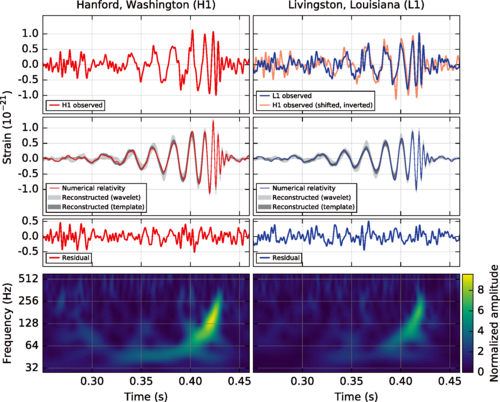
\includegraphics[width=\textwidth]{figure/BBH.png}                          
	\caption{The first detection of \ac{GW} from a binary black hole
merger by two \ac{LIGO} detectors~\cite{Abbott_2016}.}
\end{figure}      

During the second observation run of Advanced LIGO and Virgo on August 17, 2017,
the network of three detectors observed a \ac{GW} signal from a binary
neutron star merger~\cite{Abbott_2017}. The signal was first detected marginally in the Virgo
detector and in Livingston after 22\,ms and later in Hanford in another 3 ms,
limiting the sky localization to 28 square degrees. The signal frequency went
from 30\,Hz to 2048\,Hz within a minute. The total mass of merger remnant
is $2.74_\odot$ where $0.025 M_\odot$ were radiated as \ac{GW} energy at a
luminosity distance of 40\,Mpc (130 million light years). After 1.7 s a
burst of gamma rays was detected by the Fermi telescope from a same  location. Other
spectrum of \ac{EM} waves were discovered with delays ranging from few hours for optical
light to a few weeks for radio waves.  This makes the first cosmic event that
was seen in both gravitational waves and electromagnetic waves starting the era
of multi-messenger astronomy. 
\begin{figure}[bhtp!] 
        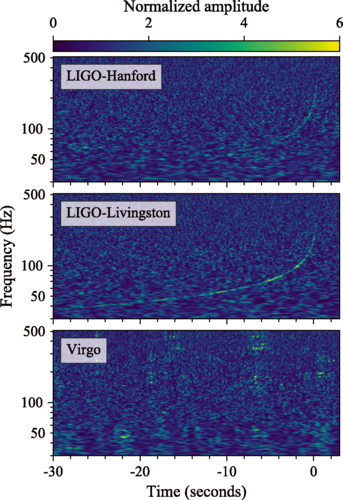
\includegraphics[width=\textwidth]{figure/GW170817.png}
	\caption{The first detection of binary neutron star merger (GW170817) by
the \ac{LIGO} detector~\cite{Abbott_2017}. The figure shows a spectrogram of the \ac{GW} event
GW170817. The signal direction was on the blind side of the VIRGO detector. This
was important to predict the sky location of GW170817.  }
        \label{GW170817}                                                             
\end{figure}      

The detection of \ac{GW} opened a new way to understand the universe. This not
only supported the Einstein Theory of General Relativity but was the first
detection of such a high mass of black hole. The neutron star collision was seen
not only in \ac{GW} but also across the \ac{EM} spectrum. This event showed the
heavier elements like uranium and gold are formed through a $r$-process
nucleosynthesis, where a nucleus gets absorbed by a heavier nucleus such as iron
and the nucleus decays into proton and electron increasing the proton number of
nucleus and forming new elements. 


%%%%%%%%%%%%%%%%%%%%%%%%%%%%%%%%%%%%%%%%%%%%%%%%%%%%%%%%%%%%%%%%%%%%%%%%%%%%%%%%%%%%%%%%%
%%%%%%%%%%%%%%%%%%%%%%%%%%%%%%%%%%%%%%%%%%%%%%%%%%%%%%%%%%%%%%%%%%%%%%%%%%%%%%%%%%%%%%%%%
%%% 							Chapter 2											  %%%
%%%%%%%%%%%%%%%%%%%%%%%%%%%%%%%%%%%%%%%%%%%%%%%%%%%%%%%%%%%%%%%%%%%%%%%%%%%%%%%%%%%%%%%%%
%%%%%%%%%%%%%%%%%%%%%%%%%%%%%%%%%%%%%%%%%%%%%%%%%%%%%%%%%%%%%%%%%%%%%%%%%%%%%%%%%%%%%%%%%

\chapter{Gravitational Waves}
Compact objects such as black holes or neutron stars warp the space-time. When
these objects move at relativistic speed, the changing warpage in space-time
propagating at the speed of light is known as gravitational
waves~\cite{thorne1995gravitational}. The detection of \acp{GW} has created a
new era in astronomy.  \acp{GW} can travel long distances without getting
absorbed or scattering whereas \acp{EM} get absorbed or scatter easily. So, the
universe that can be observed through \acp{GW} is invisible to \ac{EM}. 

\section{Theory of Gravitational Waves}
The General Theory of Relativity describes the equation of motion of a freely
falling particle as:
\begin{equation}
\frac{d^2x_\lambda}{d\tau^2}+\Gamma^\lambda_{\mu\nu}\frac{dx_\mu}{d\tau}\frac{dx_\nu}{d\tau}=0,
\end{equation}
where $\mu$ and $\nu$ are the space-time coordinates, the indices go from 0--3
and
$\tau$ is the proper time and  $\Gamma^\lambda_{\mu\nu}$ is the affine connection:
\begin{equation}
\Gamma^\lambda_{\mu\nu} =\frac{\partial x^\lambda}{\partial
x^\alpha}\frac{\partial^2x^\alpha}{\partial x_\mu \partial x_\nu},
\end{equation}

\begin{equation}
d\tau^2=dt^2 - dx^2 = -g_{\mu\nu}dx_\mu dx_\nu,
\end{equation}
where $g_{\mu\nu}$ is a metric tensor that describes space-time curvature.
\subsection{Newtonian Limit}
	For a slowly moving particle 
\begin{equation}
\frac{dx^i}{d\tau}<< \frac{dt}{d\tau},
\end{equation}
and thus,
\begin{equation}
\frac{d^2x_\mu}{d\tau^2}+\Gamma^\lambda_{00}\left(\frac{dt}{d\tau}\right)^2
\cong 0,
\end{equation}
For a stationary gravitational field, $\Gamma^\lambda_{00}$ can be written as:
\begin{equation}
\Gamma^\lambda_{00}= -1/2 g^{\mu \nu} \frac{\partial g_{00}}{\partial x^\nu},
\end{equation}	
For a weak gravitational field, we can write the metric as Minkwoski plus a small
perturbation:
\begin{equation}
g_{\mu \nu}= \eta_{\mu \nu} + h_{\mu \nu},
\end{equation}
\begin{equation}
\Gamma^\lambda_{00}= -1/2 g^{\mu \nu} \frac{\partial h_{00}}{\partial x^\nu},
\end{equation}	
\begin{equation}
\frac{d^2x_\mu}{d\tau^2}=1/2 g^{\mu \nu} \frac{\partial h_{00}}{\partial x^\nu}
\left(\frac{dt}{d\tau}\right)^2,
\end{equation}
For a stationary $\partial_0h_{00}=0$ and the perturbation $\mu=0$ component of
the last equation becomes:
\begin{equation}
\frac{d^2t}{d\tau^2}=0,
\end{equation}
This means $dt/d\tau$ is constant. And
\begin{equation*}
\eta_{\mu\nu}=
 \begin{pmatrix}
    -1 & 0 & 0 & 0 \\
    0 & 1 & 0 & 0 \\
    0 & 0 & 1 & 0 \\
    0 & 0 & 0 & 1 
 \end{pmatrix}
\end{equation*}

\begin{equation}                                                                
\frac{d^2x^i}{d\tau ^2}=1/2 \left(\frac{dt}{d\tau}\right)^2 \partial _i h_{00},
\end{equation} 

Dividing both sides by $\left(\frac{dt}{d\tau}\right)^2$, we get,
\begin{equation} \label{GR}                                                               
\frac{d^2x^i}{dt^2}=1/2 \partial _i h_{00}
\end{equation} 

This gives us the Newtonian case,
\begin{equation} \label{Newton}
\frac{d^2x}{dt^2}=-\nabla \Phi,
\end{equation}

Comparing \ref{GR} and \ref{Newton},we get,
\begin{equation} \label{eq:14}
h_{00}=2\Phi,
\end{equation}
And, comparing with the metric $g_{\mu \nu}= \eta_{\mu \nu} + h_{\mu \nu}$,
\begin{equation}\label{eq:15}
g_{00}=-(1+2\Phi),
\end{equation}
In Newtonian theory,the  gravitational potential obeys Poisson's
equation:
\begin{equation} \label{eq:16}
\nabla ^ 2\Phi = 4\pi G\rho,
\end{equation}
where $\Phi=-\frac{GM}{R}$ for a point mass like distribution and $\rho$ is a
mass density. In Newtonian mechanics mass is the only source of gravitational
field but in general relativity we need a quantity known as the stress energy
density ($T_{\mu\nu}$). And the gravitational potential can be generalized to a metric
tensor ($h_{\mu\nu}$).
In the weak field limit, the rest energy can be written as:
\begin{equation}\label{eq:17}
T_{00}=\rho
\end{equation}
From \ref{eq:14}, \ref{eq:16} and \ref{eq:17}
\begin{equation} \label{eq:18}
\nabla ^2h_{00}=-8\pi GT_{00}
\end{equation}
	
	For a vacuum the Ricci tensor $R_{\mu \nu} = 0$ since
there is no gravitational field. But the equation with matter will be:
\begin{equation} \label{eq:19}
R_{\mu \nu} = 8 \pi GT_{\mu \nu},
\end{equation}
where,
\begin{equation} \label{eq:22}
R_{\mu \nu} = \frac{\partial \Gamma ^\gamma _{\mu \nu}}{\partial x^\gamma} -
\frac{\partial \Gamma ^\gamma _{\mu \gamma}}{\partial x^\nu}+ \Gamma ^\gamma
_{\mu \nu}\Gamma ^\delta _{\gamma \delta}-\Gamma ^\gamma _{\mu \delta}\Gamma
^\delta_{\nu \gamma}
\end{equation}

In a local inertial frame, the stress-energy is conserved in curved
space-time.
\begin{equation} \label{eq:20}
\nabla ^\mu T_{\mu \nu} =0,
\end{equation}
from \ref{eq:19} and \ref{eq:20},
\begin{equation}
\nabla ^\mu R_{\mu \nu} =0,
\end{equation}
light. In \ac{GR}, Einstein field equation is written as:
\begin{equation}
R_{\mu\nu} -\frac{1}{2}g_{\mu\nu}=-\kappa T_{\mu\nu},
\end{equation}	
where $R_{\mu\nu}$ is the Ricci tensor, $g_{\mu\nu}$ is the metric tensor, R is a scalar
curvature and $T_{\mu\nu}$ is the stress energy tensor. The LHS describes the
curvature of space-time and the RHS defines the energy density.\\

\subsection{Linearized Theory of Gravity}
The last two terms in \ref{eq:22} are quadratic in $h_{\mu \nu}$ so are negligible
in linear approximation.The perturbation in Ricci tensor is given by:
\begin{equation} \label{eq:23}
\delta R_{\mu \nu} = \frac{\partial \delta \Gamma ^\gamma _{\mu \nu}}{\partial 
x^\gamma} - \frac{\partial \delta \Gamma ^\gamma _{\mu \gamma}}{\partial x^\nu}
\end{equation}
The first order perturbations in Christoffel symbols are:
\begin{equation} \label{eq:24}
\delta \Gamma ^\gamma _{\mu \nu}= 1/2 \eta^{\gamma \delta}\left(\frac{\partial
h_{\delta \mu }}{\partial x^\nu} + \frac{\partial h_{\delta \nu }}{\partial
x^\mu} -\frac{\partial  h_{\mu \nu }}{\partial x^\delta}\right),
\end{equation}
\begin{equation} \label{eq:25}
\delta R_{\mu \nu} = \frac{1}{2}\left[ -\left(-\frac{\partial^2}{\partial
t^2}+\nabla ^2\right)\tilde h_{\mu\nu} + \delta_\mu V_\nu + \delta_\nu V_\mu
\right],
\end{equation}
\begin{equation} \label{eq:26}
V_\mu = \delta_\gamma h^\gamma_\mu - \frac{1}{2}\delta_\mu h^\gamma_\gamma,
\end{equation}
	If we choose $V_\mu=0$ similar to the Lorentz gauge condition in
electromagnetism, the linearized Einstein equation becomes:
\begin{equation} \label{eq:27}
\left(-\frac{\partial^2}{\partial t^2}+\nabla ^2\right)\tilde h_{\mu\nu} = 0, 
\end{equation}

%We can define a transverse reverse of $h_{\mu \nu} 
%\begin{equation}
%\tilde h_{\mu \nu} \approx h_{\mu \nu} -1/2 \eta_{\mu \nu}h
%\end{equation}
Now, the gauge condition becomes:
\begin{equation}\label{eq:28}
\partial _\mu \tilde h^\mu _\lambda = 0,
\end{equation}
The Einstein field equation in vacuum becomes:
\begin{equation}\label{eq:29}
\left(-\frac{\partial^2}{\partial t^2}+\nabla ^2\right)\tilde h_{\mu\nu} =0
\end{equation}


\subsection{Gravitational wave radiation}
The equation \ref{eq:27} has a plane wave solution given by:
\begin{equation} \label{eq:30}
h^{\mu \nu} = A^{\mu \nu}e^{ik_\sigma x^\sigma}
\end{equation}
Here $A^{\mu \nu}$ is a tensor which has information on
polarization and amplitudes of the gravitational waves.
%  Apart from gauge
%transformation we cam use the coordinate transformation to simplify the $A_{\mu
%\nu}$
%\begin{equation}
%x^{'\mu}= x^\mu +x_i ^\mu(x)
%\end{equation}
%\begin{equation}
%\left(-\frac{\partial^2}{\partial t^2}+\nabla ^2\right)\xi_\mu(x) =0
%\end{equation}
Since $A_{\mu \nu}$ also satisfies the wave equation, the transformation will
eliminate any four components of $A_{\mu \nu}$.
\begin{equation}
\begin{aligned}
h_{ti}=0, \\
h^\nu_\nu =0,
\end{aligned}
\end{equation}
or $A_{ti}=0$ and $A_\nu ^\nu=0$. Using the gauge condition $V_\mu =0$
\begin{equation}
\begin{aligned}
V_t=\frac{\partial h^t _t}{\partial t}=0,\\
V_i=\frac{\partial h^j _i}{\partial x^j}=0
\end{aligned}
\end{equation}
From the above equation,
\begin{equation}                                                                
\begin{aligned} 
A_{tt}=0, \\
k_j A_{ij}=0,
\end{aligned}                                                                   
\end{equation} 
This means the gravitational waves are transverse and the vector k
determines the direction of wave propagation. The time component vanishes and
since the waves are transverse $A_{zi}=0$ assuming $\vec{k}=(0,0,\omega)$. Now,
we are left with a $2 \times 2$ symmetric matrix in the xy-plane with zero trace. With coordinate transformation and gauge conditions, the linearized
Einstein equation can be written in terms of two dimensionless amplitudes
$h_+$ and $h_\times$ and two polarization vectors $\hat e_+$ and $\hat
e_\times$. Defining

\begin{equation*}                                                               
h_{\mu\nu}=                                                                  
 \begin{pmatrix}                                                                
    0 & 0 & 0 & 0 \\                                                           
    0 & h_+ & h_\times & 0 \\                                                            
    0 & h_\times & -h_+ & 0 \\                                                            
    0 & 0 & 0 & 1                                                               
 \end{pmatrix}                                                                  
\end{equation*} 
The metric $h_{\mu\nu}$ can be written as the sum of two polarization components.   
\begin{equation}
h_{\mu\nu}=h_+\hat e_+ +h_\times \hat e_\times,
\end{equation}
The polarization tensors are defined as:
\begin{equation}
\begin{aligned}
\hat e_+ = \hat e_x \otimes \hat e_x - \hat e_y \otimes \hat e_y, \\
\hat e_\times = \hat e_x \otimes \hat e_y + \hat e_y \otimes \hat e_x,
\end{aligned}
\end{equation}
Or we can write the metric perturbation in matrix form:
\begin{equation*}                                                               
h_{\mu\nu}=     
 \begin{pmatrix}                                                                
    0 & 0 & 0 & 0 \\                                                            
    0 & 1 & 0 & 0 \\                                                            
    0 & 0 & -1 & 0 \\                                                            
    0 & 0 & 0 & 0                                                               
 \end{pmatrix}
h_+  
+
 \begin{pmatrix}                                                                
    0 & 0 & 0 & 0 \\                                                            
    0 & 0 & 1 & 0 \\                                                            
    0 & 1 & 0 & 0 \\                                                            
    0 & 0 & 0 & 0                                                               
 \end{pmatrix}
h_\times                                                                  
\end{equation*} 

\begin{figure}[h!]                                                              
	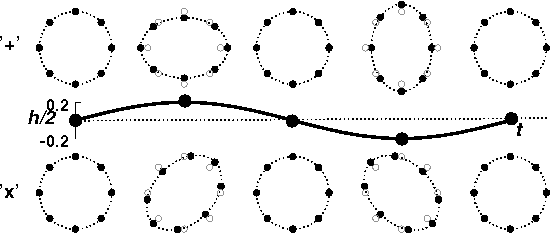
\includegraphics[width=\textwidth]{figure/polarization.png}
	\caption{The figure shows the effect of passing a gravitational wave
through a ring of particles. The top figure shows the plus polarization and the
bottom shows cross polarization. Figure from ~\cite{Schutz}}                                                     
        \label{fig:polarization}
\end{figure}

	The effect of a passing gravitational wave is to compress and stretch
alternately in the transverse directions. Let us assume a ring of particles in
the xy
plane and a \ac{GW} traveling in the  z-direction. This will cause the
ring to contract along the x-axis at the same time it expands along the y-axis. These
contractions and expansions will oscillate as  gravitational waves pass. 

\subsection{Gravitational Wave Luminosity}
\ac{GW} energy cannot be localized perfectly,
however we can say a certain amount of energy is contained in a region of
several wavelength extent. The stress energy of \acp{GW} is given by:
\begin{equation}
T_{\mu\nu}^{GW} = \frac{1}{32\pi}\left\langle
h_{jk,\mu}^{TT}h_{jk,\nu}^{TT}\right\rangle
\end{equation}
where <> means averaging over several wavelength and TT means Transverse
Traceless.
For a wave propagating in the z-direction, 
%it has three non-zero components.
\begin{equation}
T_{00}^{GW}=\frac{1}{16\pi}<\dot{h}_+^2+\dot{h}_\times ^2>,
\end{equation}
If we suppose \acp{GW} has a frequency $f$ and the amplitude $h_+ = h_\times = h$,
then, $\dot{h}_+ = \dot{h}_\times = \frac{1}{2}(2\pi fh)^2$
S, and the energy density of the \acp{GW} is:
\begin{equation}
T_{00}^{GW} = \frac{\pi}{4}\frac{c^3}{G}f^2 h^2=0.3\left(\frac{f}{1kHz}\right )^2
\left(\frac{h}{10^{-21}}\right )^2\frac{W}{m^2}
\end{equation}
\\
The spin down limit for Crab amplitude strain is $h\approx 3 \times 10^{-24}$
from
$r$-mode frequency around 41Hz. So the total energy flux radiated by Crab pulsar
on earth due its loss of rotational energy will be
$4.5\times10^{-9}\frac{W}{m^2}$.

\subsection{Generation of Gravitational Waves}

	The \ac{GW} is quadrupole in nature as the mass( monopole) and
momentum (dipole) are conserved. In Electromagnetism we can have dipole
radiation as there can be positive and negative charges.
The Einstein quadrupole formula for \acp{GW} can be written as:
\begin{equation}\label{eg:strainamplitude}
h_{\mu\nu}= \frac{2}{r}\frac{G}{c^4}\ddot{I}_{\mu\nu}^{TT}
\end{equation}
where $I_{\mu\nu}$ is the quadrupole moment.


Using the Einstein quadrupole formula the \ac{GW} luminosity can be written
as:
\begin{equation}
\frac{dE}{dt} =
-\frac{1}{5}\frac{G}{c^5}\left\langle\dddot{I}_{\mu\nu}\dddot{I}_{\mu\nu}\right\rangle
\end{equation}
The expression for power radiated by \ac{GW} is similar to the power radiated by the electric
dipole, where the expression is written as
$\frac{dE}{dt}=\frac{\mu_o}{6\pi}\left\langle \ddot{p}^2\right\rangle$, where p is an electric
dipole. Like we discussed earlier, in \ac{GW} the first non vanishing term is
the quadrupole whereas in \ac{EM} it is the dipole.

\section{Indirect evidence of Gravitational Waves}
	
Gravitational radiation will remove the energy from a binary system or a
rotating neutron star. Hulse and Taylor cite found a binary system with a
neutron star and a pulsar named PSR B1913+16 whose orbital period was decaying which
can be explained by \acl{GW} emission. Both companions have a mass of $1.4 M_o$
with a orbital period of 8 hrs. The rate of orbital decay
$dP/dt\approx10^{-12}$\,s/s 
as predicted by General relativity within 0.2\%~\cite{1975ApJ...195L..51H}. The disparity between predicted
and observed was due to the poor measurement of distance and proper motion of
pulsar as well as the radius of Sun's galactic orbit~\cite{Weisberg_2010}. This discovery led to
the 1993 Nobel prize in Physics for Russell Hulse and Joseph Taylor.
\begin{figure}[bht!]
	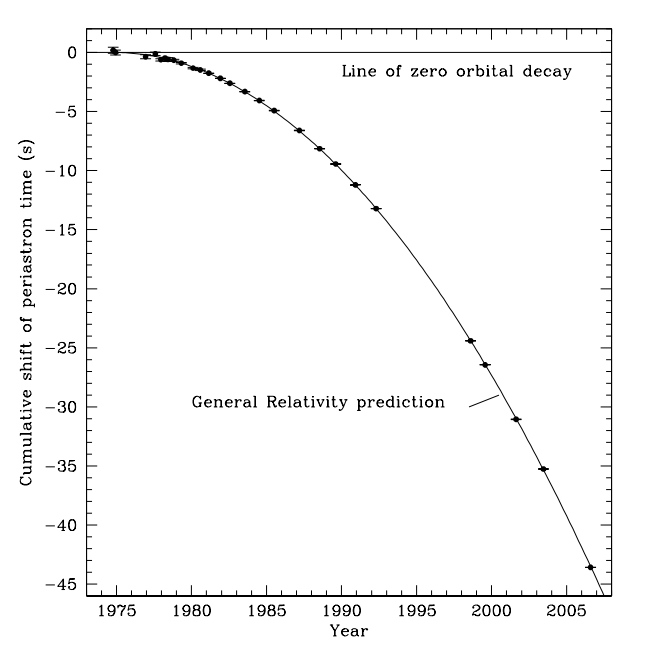
\includegraphics[width=\textwidth]{figure/pulsar.png}
	\caption{The orbital decay of binary pulsars $ PSR B1913+16$ due to the
loss of \ac{GW} energy. The image is from \cite{Weisberg_2010}}
\end{figure}  

\section{Gravitational Wave Detector}
The challenge of detecting \ac{GW} is the amplitude of \ac{GW} are really small
 ($\approx10^{-18}$\,m) displacement, so the noise in the detector can easily mask the signal.
\ac{GW} detectors include resonant bars, interferometers, and pulsar
timing arrays. 

\subsection{Resonant bars}

The resonant bar works on a simple concept. When the frequency of a
\ac{GW} matches the bar the detector will resonate and ring like a bell. This
was the first \ac{GW} detector built by Joseph Weber, consisting of an
aluminum bar of 2 meters, and pizezo-electric sensors. But the
noises of strain amplitude $10^{-16}$ surpasses the strong \ac{GW}
signals$10^{-21}$ by many orders of
magnitude and the GW frequency is only in principle detectable at the resonant
bar frequency. Weber claimed the detection of \ac{GW} coming from the center of
 the galaxy, which led to the construction of similar detectors by other physicist. But none of the
other detectors saw any signals and the claim must likely was a glitch in the
instrument.
\subsection{Interferometer}
\ac{GW} interferometry works on the simple principle
developed by Michelson and Morley and consists of a laser, beam splitter,
mirror and a detector. The laser emits a monochromatic wave towards a beam
splitter which splits the beam into two perpendicular directions. The beam gets
reflected by the mirrors, passes through the beam splitter and meets at the
photo-detector. The two waves superimpose at the detector to give constructive or
destructive interference depending on the phase difference. When \acp{GW} passes
the interferometer the relative length between two arms oscillates changing the
intensity of light at photo-detector. Actually, the light reflects many times
between mirrors before they combine making the effective length of the
interferometer more than its physical arm length.

There are two working \ac{LIGO}, one at Livingston, Louisiana and Hanford, Washington 
separated by 3000\,km. Each arm of the interferometers is 4\,km in length. The
VIRGO interferometer in Italy and KAGRA (3\,km arms length) in Japan are also
operational. It takes at least three detectors to determine the sky location of 
\ac{GW} sources, its intrinsic amplitude, polarization angle and the
distance.~\cite{Schutz_2011}. But for the long lived \ac{CW} signals the Doppler effect
due to Earth's orbital and sidereal motion can help to locate the source. The
network of detector will also build up the signal to noise ratio(SNR) as the
network SNR is the sum of individual detector SNR~\cite{Schutz_2011}.
\begin{equation}
\rho_N^2=\sum_{k=1}^N \rho_k^2 ,
\end{equation}

\subsubsection{Principle of Interferometer}
This section is based on the ~\cite{Sathyaprakash_2009}. The
\ac{GW} interferometer is based on the principle that passing of \ac{GW} will
change the length of the arm of the interferometer. If there is a \ac{GW}
passing then the arrival time of reflected laser light will be different than when no
\ac{GW} passes. Lets assume a \ac{GW} is travelling in z-direction with +
polarization, then the metric can be written as:
\begin{equation}
ds^2= -c^2dt^2+[1+h_+(\frac{z}{c}-t)]dx^2+[1-h_+(t-\frac{z}{c})]dx^2+dz^2,
\end{equation}
Lets assume a photon is emitted at time $t_{start}$ and travels
in the x-direction of interferometer and returns back time at $t_{return}$. So,
the photon travels in a null world line with dy=dz=0.
\begin{equation}
\left(\frac{dx}{dt}\right)^2=\frac{c^2}{1+h_+},
\end{equation}
Solving the above equation (for details \cite{Schutz:1985jx}),
\begin{equation}
\frac{dt_{return}}{dt_{start}}=1+\frac{1}{2}[h_+(t_{start}+2L/c)-h_+(t_{start})],
\end{equation}
%\begin{equation}
%\frac{dt_{return}}{dt}=1+\frac{1}{2}{(1-\cos{\theta})h_+(t+2L)-(1+\cos{\theta})h_+(t)
%+ 2\cos{\theta} h_+[t+L(1-\cos{\theta})]}
%\end{equation}
%For a small L approximation compare to the wavelength of \ac{GW}.
%\begin{equation}
%\frac{dt_{return}}{dt} =1+\sin{\theta}^2 L \dot{h}_+ (t)
%\end{equation}
%Or for the x-arm, it can be written as:
%\begin{equation}
%\left(\frac{dt_{return}}{dt})\right)_{x-arm}=1+L\hat{e}_x.\dot{h}.\hat{e}_x
%\end{equation}
%Similarly for the y-arm:
%\begin{equation}                                                                
%\left(\frac{dt_{return}}{dt}\right)_{y-arm}=1+L\hat{e}_y.\dot{h}.\hat{e}_y  
%\end{equation}  
%The difference between the arrivals time of photons from the two arms is:
%\begin{equation}
%\left(\frac{d\delta t_{return}}{dt}\right)=L(\hat{e}_x\otimes\hat{e}_x-(\hat{e}_y\otimes\hat{e}_y)\dot{h}
%\end{equation}
%Or the path difference between two arms as measured by the central observer's:
%\begin{equation}
%\delta t_{return}(t)=d:h
%\end{equation}
%where $d=L(\hat{e}_x\otimes\hat{e}_x-(\hat{e}_y\otimes\hat{e}_y)$ and 
%$d:h=d_{lm}h_{lm}$
%\\
%This can be written in terms of the change in length of two arms:
%\begin{equation}
%\delta L_{return}(t)=\frac{1}{2}d:h 
%\end{equation}
The above expression can be written in terms of interferometer arm. When gravitational wave passes through a detector. The one arm
of the interferometer gets stretched (lets say x-arm) by
$\delta x=\frac{1}{2}h_+L$ and the other arm gets squeezed by $\delta y=-\frac{1}{2}h_+L$  

\subsubsection{Interferometer antenna pattern}
\ac{GW} astronomy is done with combinations of detectors around the globe. The
\ac{GW} polarization might not be same in all detector frames, so it is more
convenient to choose a polarization tensors in the some sky plane with respect
to \ac{GW} sources. Let $\hat\epsilon_+$ and $\hat\epsilon_\times$ be two
polarization tensor in sky frame as shown in figure \ref{fig:polarization}. Let
$\psi$ be the rotation angle from detector frame to the source frame also known
as polarization angle.
\begin{equation}
\begin{aligned}
\epsilon_+ = e_+cos2\psi + e_\times sin2\psi, \\
\epsilon_\times = -e_+sin2\psi + e_\times cos2\psi.
\end{aligned}
\end{equation}
\begin{figure}[h!]
	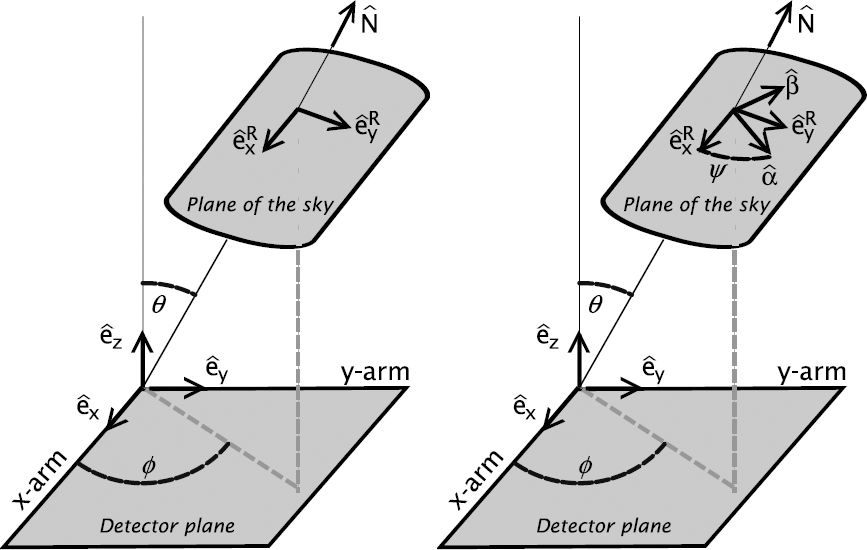
\includegraphics[width=\textwidth]{figure/antennae.jpg}
	\caption{The left figure shows the basis vector in the sky plane with
respect to the detector frame. The right figure shows the effect of rotation of
the basis vector of sky plane by angle $\psi$. Image from
~\cite{Sathyaprakash_2009}}
\end{figure}  

Let $F_+$ and $F_\times$ be the antennae pattern functions on the sky frame
defined as:
\begin{equation}
F_+=d:e_+,  F_\times=d:e_\times
\end{equation}
The maximum value of $F_+$ and $F_\times$ is 1. We can define $\theta$ \&
$\phi$ to be a spherical coordinates in the detector's reference frame. We can write
the antenna pattern in the detector frame by setting $\psi=0$ and using the
rotation matrix
\begin{equation*}                                                               
R_\beta^\alpha=                                                                  
 \begin{pmatrix}                                                                
    \cos\phi & \sin\phi & 0 \\                                                            
    -\cos\theta \sin\phi & \cos\theta \cos\phi & \sin\theta \\                                                            
    \sin\theta \sin\phi & -\sin\theta \cos\phi & \cos\theta                                                              
 \end{pmatrix}                                                                  
\end{equation*}   

For a plus polarization it is useful to define $t_{\alpha\beta}= R^{-1}e_+R$

\begin{equation*}                                                               
\begin{split}
t_{\alpha\beta} & =                                                                  
 \begin{pmatrix}                                                                
    \cos\phi & \sin\phi & 0 \\                                                            
    -\cos\theta \sin\phi & \cos\theta \cos\phi & \sin\theta \\                                                            
    \sin\theta \sin\phi & -\sin\theta \cos\phi & \cos\theta                                                              
 \end{pmatrix}^T                                                                  
\begin{pmatrix}                                                                
    1 & 0 & 0 \\                                                            
    0 & -1 & 0 \\                                                            
    0 & 0 & 0                                                               
 \end{pmatrix}       
 \begin{pmatrix}                                                                
    \cos\phi & \sin\phi & 0 \\                                                     
    -\cos\theta \sin\phi & \cos\theta \cos\phi & \sin\theta \\                        
    \sin\theta \sin\phi & -\sin\theta \cos\phi & \cos\theta                           
 \end{pmatrix}\\  
            &=
     \begin{pmatrix}                                                                 
    \cos^2\phi-\cos^2\theta\sin^2\phi & (1+\cos^2\theta)\sin\phi\cos\phi &
\sin\theta\cos\theta\sin\phi \\                                                                
    (1+\cos^2\theta)\sin\phi\cos\phi & \sin^2\phi-\cos^2\theta\cos^2\phi &
-\sin\theta\cos\theta\cos\phi \\                                                               
    \sin\theta\cos\theta\sin\phi & -\sin\theta\cos\theta\cos\phi & -\sin^2\theta                                                                   
 \end{pmatrix}     
\end{split}     
\end{equation*}   
So, the antenna pattern for the plus polarization is $F_+$
\begin{equation}
\begin{split}
F_+ & ==1/2t_{\alpha\beta}S_+\\
& = (1+\cos^2\theta)\cos2\phi
\end{split}
\end{equation}
Similarly for the cross polarization:
\begin{equation}
F_\times=\cos\theta\sin2\phi
\end{equation}
In the source frame where $\psi\neq0$, the antennae pattern is given by:
\begin{align}
F_+=\frac{1}{2}(1+\cos^2\theta)\cos2\phi\cos2\psi-\cos\theta\sin2\phi\sin2\psi,\\
F_\times=\frac{1}{2}(1+\cos^2\theta)\cos2\phi\sin2\psi-\cos\theta\sin2\phi\cos2\psi,
\end{align}

\subsubsection{Noises in Interferometer}

The amplitudes strain of recently detected binary black-hole mergers are
of order $h \approx10^{-21}$. When \ac{GW} passes by, the change in arm length of
interferometer is $10^{-18}$\,m thousands times smaller than the diameter of proton. This small
change in length due to \acp{GW} can be easily drowned by different sources of
noise. The LIGO arms consist of tubes evacuated to one trillionth of
atmospheric pressure. This is important as even a few molecules of gas will
scatter the laser beam and the moving air hitting the mirror will change the
length travelled by the laser beam mimicking \ac{GW} signal.
 At frequencies (below 10 Hz) the seismic noise including earth
quake and other ground vibrations can move the mirrors, disturbing the \ac{GW}
signal. LIGO uses both active and passive damping to isolate signal from noise.
Active damping includes sensors that track ground vibration and move the
test mass in and out of phase to cancel the noise. The passive damping suspends the
40kg mirror by a four pendulum stack to isolate the mirror from noise. Other sources of
noise are thermal noise (internal vibration and heating of mirrors due to the laser)
and shot noise (uncertainty in number of quantized photons). 
Other sources of noise are narrow spectral lines that might imitate as \acp{CW}.
This will be discussed later in chapter~\ref{}. Lines are produced by power
mains, blinking LEDs, hardware injections and resonance modes of mirror
suspensions among others. Some of the instrumental lines are shown in \ref{fig:CWnoise}
\begin{figure}[bht!]
	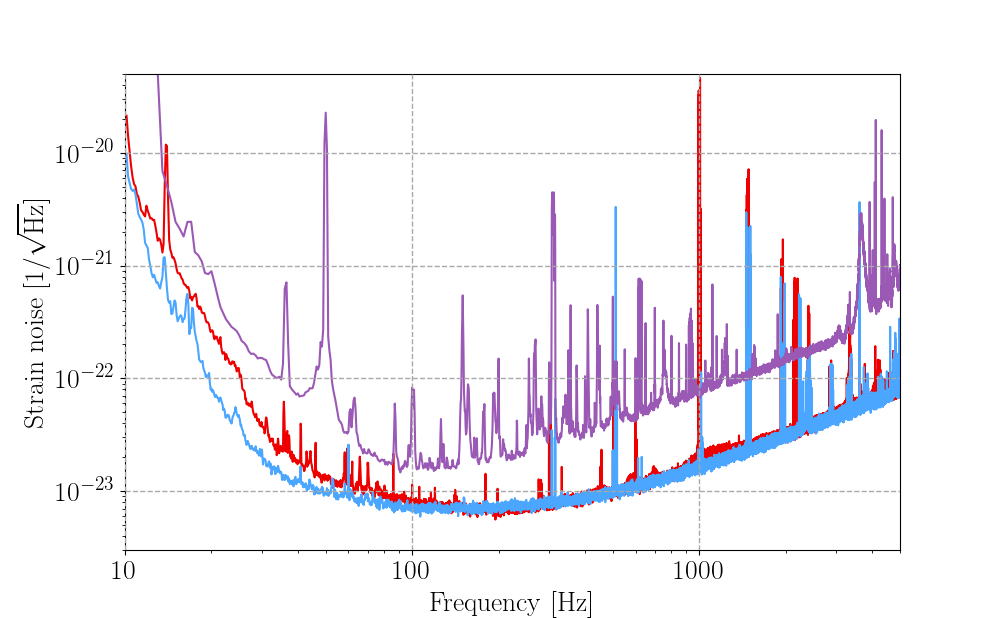
\includegraphics[width=\textwidth]{figure/CWnoise.png}
	\caption{The noise curve for the Livingston, Hanford and Virgo
interferometer during the \ac{O2} run. The spectral lines include known sources such as
60 Hz power line, blinking LEDs, calibration lines and violin modes. Figure from
~\cite{Abbott_2019} }
	\label{fig:CWnoise}
\end{figure}

\section{Sources of Periodic gravitational waves}
Continuous gravitational wave amplitudes are weaker than those of violent black
hole merger. But continuous waves lives for a longer time, so a longer
observational time is possible. The sources of continuous waves include
rotating neutron stars. A
rotating neutron star will emit a gravitational waves due to a deviation from
axisymmetry (mass quadrupole) or from a fluid oscillation inside the neutron
star (current quadrupole). 

\subsection{Neutron Stars}

Neutron stars are the densest material objects in the universe. The density in
the inner core is around $10^{15} g/cm^3$,
which is 3 times nuclear density. It drops to few $g/cm^3$ at the crust. Neutron
stars
are formed in Type II supernova explosions of 
star above $8M_\odot$.~\cite{Lattimer_2004}. When the remnant core
mass exceeds the Chandrasekhar limit$(1.44M_\odot)$. Then the electron
degeneracy pressure cannot withstand the gravitational pressure. Neutron star
masses range from 1--2\,$M_\odot$ and radius of 10--14\,km which depends on
the poorly known equation of state of superdense matter. 
	
The neutron star structure can be divided into outer and inner crust and outer, inner
core. The atmosphere of neutron star varies
from few a cm depth in hot \ac{NS}$(T\sim3\times10^6K)$ to a few millimeters in cold one
$(T\sim3\times10^5K)$~\cite{Haensel:2007yy}. The radiation from this atmosphere gives valuable
information on \ac{NS} surface temperature, chemical composition, magnetic
field, mass and radius. The outer crust goes up to a density of
$\rho=10^{11}g/cm^3$ and contains neutron with nucleus in non degenerate
electron gas~\cite{1976ApJ...208..550P}. The inner crust
can be up to a kilometer in depth. Its density might reaches saturation nuclear
density$(\rho_o=2.8\times10^{14}g/cm^3)$ and it consists of
electrons, free neutrons and neutron-rich atomic nuclei. The outer core might be
several kilometers deep and its density can reach up to $5\times10^{14}g/cm^3$.
It is
primarily rich in neutrons. The inner core's density might reach $10\rho_o$ and
at this extreme matter density it is hard to predict the composition. It might
still be dominated by neutrons, or it might feature heavier baryons (hyperons)
or free quarks. 

\subsection{Pulsars}
Pulsar are the rotating neutron star that produce a narrow \ac{EM} pulse that
acts like a lighthouse beam. When the narrow beam sweep to the line of sight of
the earth, we see the pulsation.  It was discovered by Jocelyn Bell in 1967, she
was seeing a continuous pulse every time the radio antennae was pointed to the
line of sight of pulsar. The pulsar are one of the most precise clock in the
universe. The spin period increases slowly due to the loss of rotational energy
in powering the nebulae, radiating gravitational waves. 

The pulsar magnetic moment are not aligned with the rotational axis, so the
magnetic moment changes when the pulsar rotates. This time varying magnetic
moment radiates energy known as magnetic dipole radiation. The power radiated by
pulsar in magnetic dipole radiation is:
\begin{equation}
P= \frac{B^2R^6\Omega^4\sin{\alpha}^2}{6c^3}
\end{equation}
where, B is a magnetic field, R is the radius, $\Omega$ is a rotational
frequency, $\alpha$ is angle between pulsar rotational axis and magnetic axis,
and c is the speed of light.  

The energy loss of pulsar can be estimated by the slowing down of pulsar
frequency. The energy of pulsar is written as :$E=\frac{1}{2} I \nu^2$. The
typical value of moment of inertia (I) of neutron star is $10^{38}$\,kg m$^2$. The
derivative of energy gives the rotational energy loss.
\begin{equation}
\frac{dE}{dt}= I\nu\dot{\nu}
\end{equation}

For a Crab pulsar of $\nu=29.65Hz$ and $\dot{\nu}= -3.68\times10^{-10}Hz/s$, the
rotational energy loss is $4.33\times10^{31}$W. Most of the Crab rotational energy
are lost in powering Crab nebulae in synchrotron and inverse Compton radiation.
Only $1\%$ are lost  in the observed pulsation due to electromagnetic radiation.
The characteristic age of pulsar is given by:
\begin{equation}
t= \frac{1}{n-1}\frac{\nu}{\dot{\nu}}
\end{equation} 
The term n is known as braking index given by, $n=\nu\ddot{\nu}/\dot{\nu}^2$. 
The braking index value is n=1 for pulsar wind, n=3 for magnetic dipole
radiation, n=5 for mass quadrupole \ac{GW} radiation and n=7 for current
quadrupole radiation.

\section{Gravitational Wave from Neutron Star}
An individual spinning neutron star can emit a quasi-monochromatic \acp{GW} by
various mechanism. The signals strength are weak but long lived. The frequency
of continuous \acp{GW} decreases slowly due the loss of rotational energy. The
detection on continuous \ac{GW} will give a valuable information on neutron star
equation of state.

\subsection{Mountains on neutron stars}
A non-axisymmetric rotating star can produce a periodic \ac{GW} due to a time
varying mass quadrupole. Let us consider a asymmetric neutron star rotating
around z-axis with a moment of inertia $I_{xx}\neq I_{yy}=I_{zz}$ and
ellipticity,$\epsilon=(I_{xx}-I_{yy})/I_{zz}$

\begin{figure}[h!]                                                            
        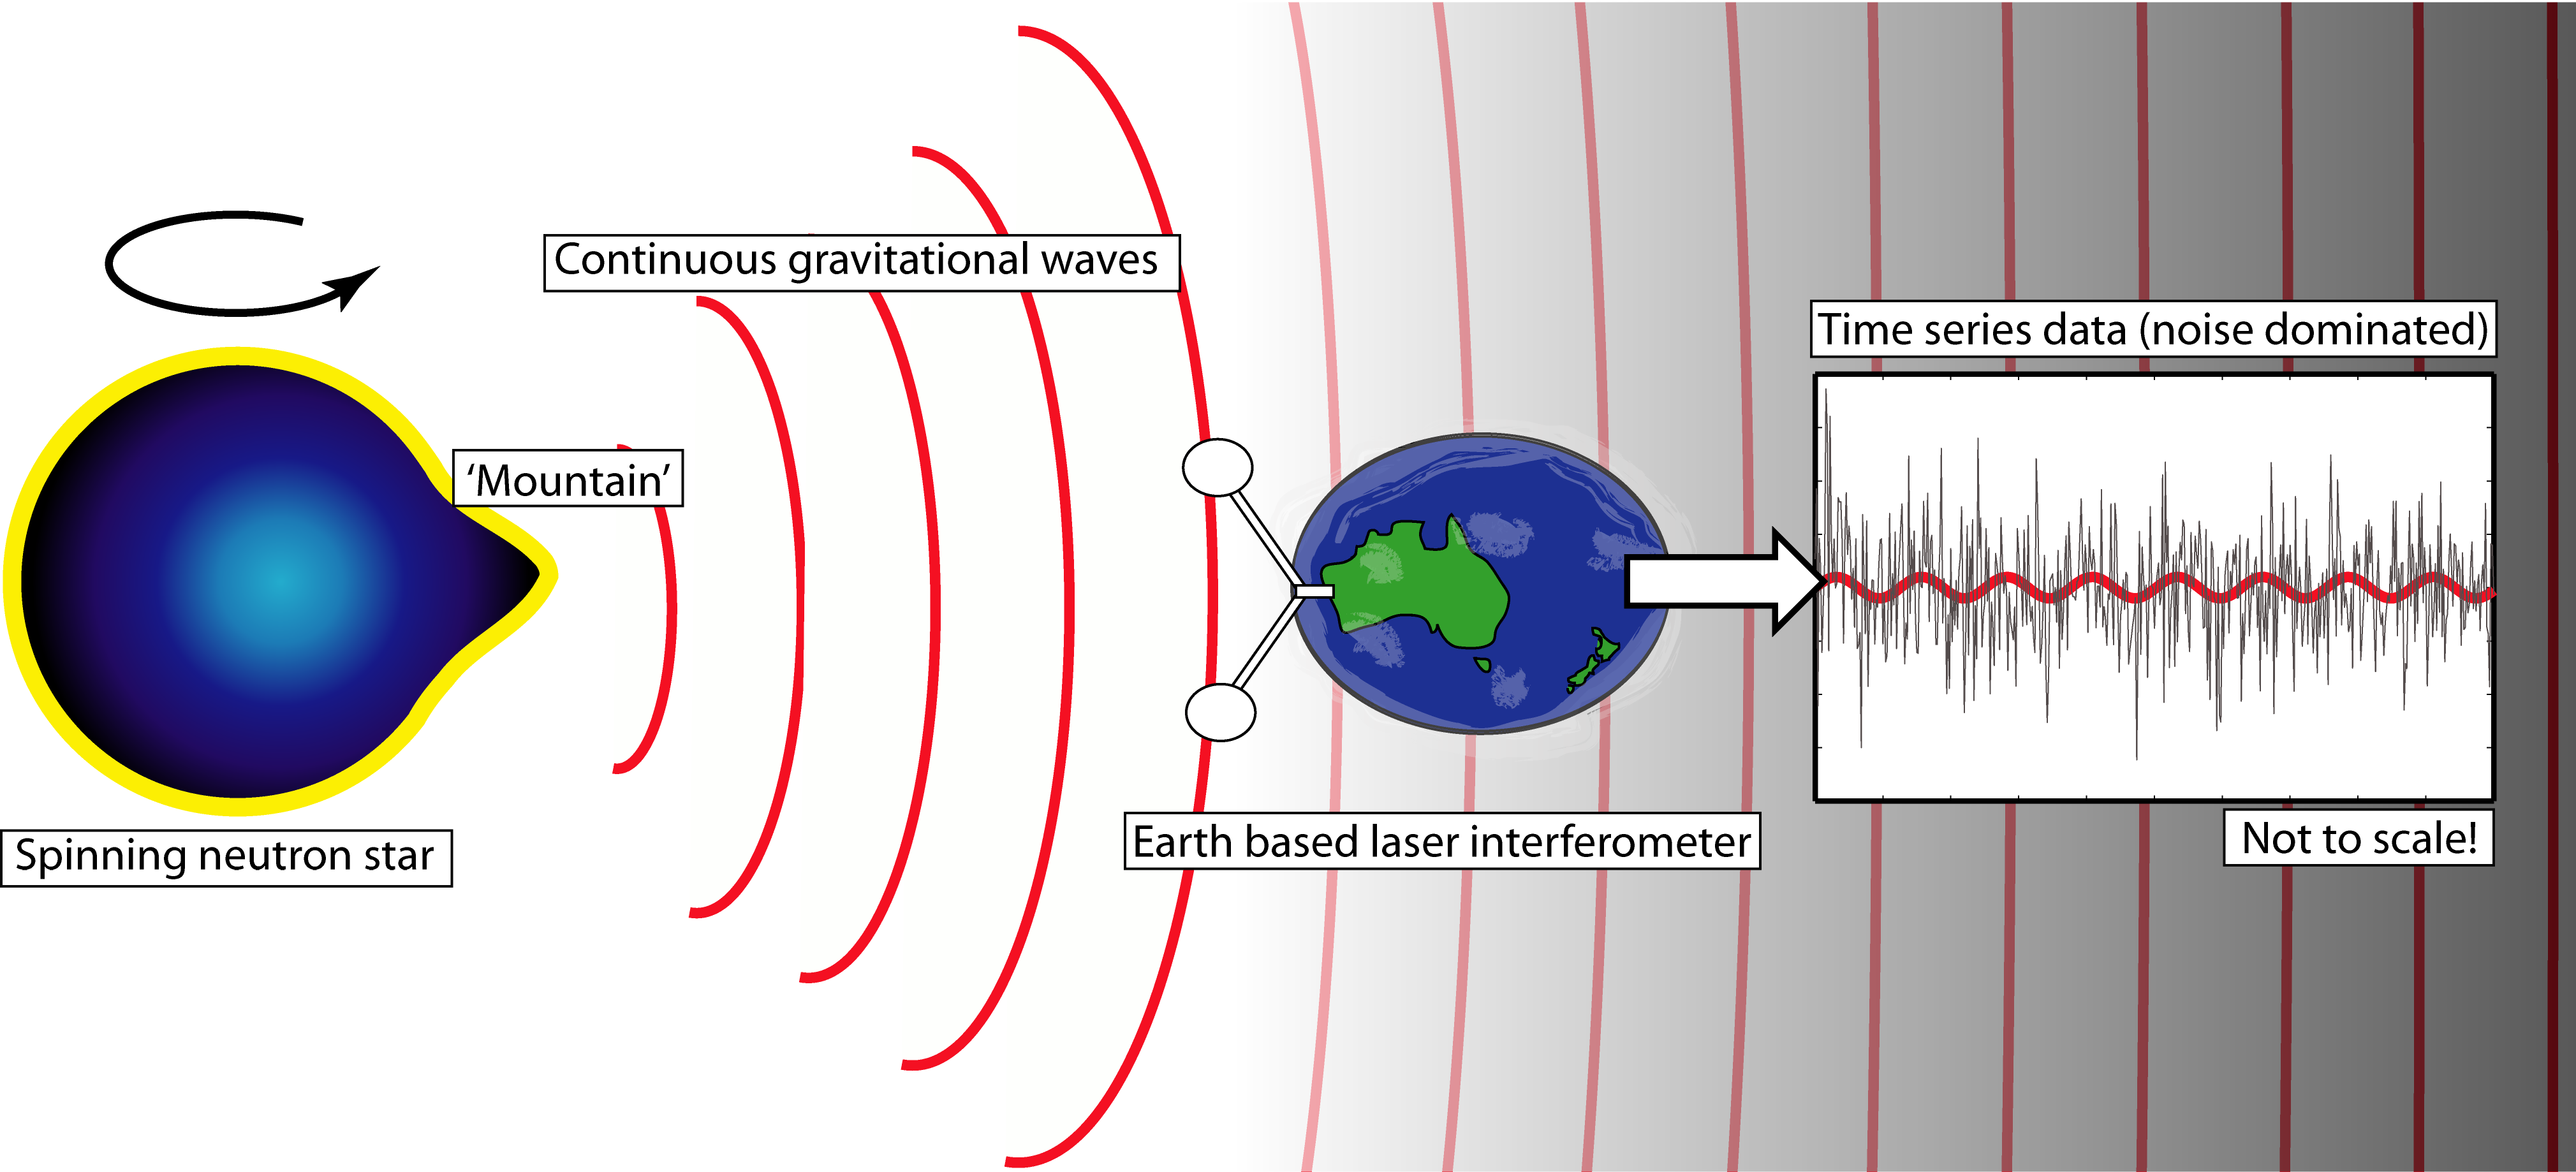
\includegraphics[width=\textwidth]{figure/CW.png}                 
        \caption{continuous gravitational wave emission due to mountain in
neutron star. Image:Ra Inta}
        \label{fig:CW}                                                 
\end{figure}     

The principle of moment of inertia needs to be transform from rotating frame to 
the inertial frame as \acp{GW} lives in an inertial frame~\cite{PhysRevD.20.351}. 
We will use a rotation matrix R for transformation.
$I_{inertial}= R^T I R$
where, 
\begin{equation}
R=
\begin{pmatrix}
\cos\theta & \sin\theta & 0 \\
-\sin\theta & \cos\theta & 0 \\
0 & 0 & 1
\end{pmatrix}
\end{equation}

\begin{equation}
I_{inertial}=
\begin{pmatrix}
(I_{xx}-I_{yy})(\cos2\theta -1) & \frac{1}{2}\sin2\theta(I_{xx}-I_{yy}) & 0 \\
\frac{1}{2}\sin2\theta(I_{xx}-I_{yy}) & (I_{xx}-I_{yy})(1-\cos2\theta) & 0  \\
0 & 0 & I_{zz}
\end{pmatrix}
\end{equation}

The double derivative of moment of inertia is given by:
\begin{equation} \label{2ndMI}
I_{\mu\nu}=-16\pi ^2f^2(I_{xx}-I_{yy})
\begin{pmatrix}
0 & 0 & 0 & 0 \\
0 & cos(4\pi\omega t) & 2sin(4\pi\omega t) & 0 \\
0 & 2sin(4\pi\omega t) & -cos(4\pi\omega t) & 0 \\
0 & 0 & 0 & 0 \\
\end{pmatrix}
\end{equation}

The gravitational wave luminosity of rotating is:
\begin{equation}\label{GWLuminosity}
L= \frac{G}{c^5}<\dddot{I}_{\mu\nu}\dddot{I}^{\mu\nu}>
\end{equation}

Combining \ref{2ndMI} \& \ref{GWLuminosity}, we get,
\begin{equation}\label{Lgw}
L_{grav}= \frac{32}{5}\omega ^6 I_{zz}^2\epsilon ^2
\end{equation}
where, $\epsilon =\frac{I_{xx}-I_{yy}}{I_{zz}}$ is defined as ellipticity. When
ellipticity is zero, there will not be any gravitational wave emission as there
won't be any non-axisymmetric components.

The gravitational wave frequency from non-axisymmetric neutron star will be
twice the spin frequency as the mass deformation will repeat after half
revolution.

The amplitude strain of \ac{GW} is given by~\ref{eg:strainamplitude}:
\begin{equation}
h_{\mu\nu}=\frac{2G}{c^4d}\ddot{I}_{\mu\nu}
\end{equation}


\begin{equation} \label{2ndMI}
h_{\mu\nu}=-\frac{32\pi ^2\omega^2 \epsilon I_{zz}}{d}
\begin{pmatrix}
0 & 0 & 0 & 0 \\
0 & \cos(4\pi \omega t)(1+\cos ^2i) & 2\sin(4\pi \omega t)\cos i & 0 \\
0 & 2\sin(4\pi\omega t)\cos i & -\cos(4\pi\omega t)(1+\cos ^2i) & 0 \\
0 & 0 & 0 & 0 
\end{pmatrix}
\end{equation}
where i is the inclination angle which is the angle between the spin axis and
the inertial observer. When $i=90^\circ$, the amplitude strain will be:
\begin{equation}
h_0=\frac{4\pi ^2Gf^2 \epsilon I_{zz}}{c^4d}
\end{equation}
\subsection{$r$-modes}
The other kind of \ac{GW} emission is the non-radial oscillation of fluid
inside neutron star known as $r$-modes. These modes are unstable to
gravitational radiation so probably lives for a long time in a rotating neutron
stars. These osillating modes carry away the rotating energy from neutron star
slowing down its spin frequency. R-modes amplitude grow up to a large value just
after the formation of core collapse neutron star. This might explain the
slowing down of spin frequency of neutron star that are born in a Keplerian
limit.The detection of $r$-modes will help to
understand the interior and composition of neutron star. It may even give the
unknown spin frequency of neutron stars where the narrow beam of light is not
pointing towards earth. The theory of $r$-modes will be discuss in more detain in next chapter.
\begin{figure}
\centering
	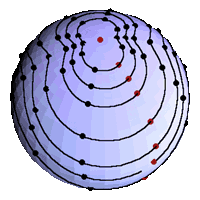
\includegraphics[width=0.4\textwidth]{figure/333.png}
	\caption{$r$-modes pattern of a oscillating neutron star. Image: Chad
Hanna/ Ben Owen}
\end{figure}
The \ac{GW} luminosity due to $r$-mode emission can be written in geometrized
unit(c=G=1) as~\cite{Owen:2010ng}:
\begin{equation}\label{eq:modeenergy}
\frac{dE}{dt}=\frac{4}{25}M R^3 \alpha \omega^8\tilde{J}
\end{equation}
where M, R, $\omega$, are the mass, radius, angular velocity of the neutron
star.$\alpha$ is the amplitude of $r$-modes. $\tilde{J}=1.635\times10^{-2}$ and
defined as~\cite{Owen:1998xg}:
\begin{equation}
\tilde{J}=\frac{1}{MR^3}\int_0^R\rho r^6dr.
\end{equation}
The rotational kinetic of neutron star can be written as:
$E=1/2I_{zz}\omega^2$. So, taking the derivative of energy will give:
\begin{equation}\label{eq:rotenergy}
\frac{dE}{dt}= I_{zz}\omega\dot{\omega}
\end{equation}
Combining Eqn ~\ref{eq:modeenergy} and \ref{eq:rotenergy}.
\begin{equation}\label{eq:braking}
\dot{\omega}=\frac{4}{25 I_{zz}}M R^3 \alpha\tilde{J} \omega^7 
\end{equation}
Let us define $4/(25 I_{zz})M R^3 \alpha\tilde{J}=K$, so\\
$\dot{\omega}=K \omega^7$
Taking derivative of \ref{eq:braking}.
\begin{equation}
\ddot{\omega}= K\omega^6\dot{\omega}
\end{equation}
Subsituting $K=\dot{\omega}/\omega^7$
\begin{equation}\label{eq:modebraking}
\frac{\omega\ddot{\omega}}{\dot{\omega}^2}=7
\end{equation}
The equation ~\ref{eq:modebraking} is defined as braking indices (n), and the
braking indices of pulsar emitting $r$-modes is 7. Braking torque generally
defines the spin down torque due to emission of energy. The braking indices for
pulsar wind is 1, 3 for magnetic dipole radiation and 5 for gravitational waves 
emission due to mountain on neutron stars. From eqn ~\ref{Lgw} we can easily
calculate the braking indices for \ac{GW} due to mountains on neutron star.
\subsubsection{$r$-mode amplitude}
The energy of the $r$-mode is proportional to the dimensionless amplitude
parameter $\alpha$. The amplitude parameter is roughly equal to the ratio of
velocity perturbation ($\delta v$) to the rotational velocity at equator. The
intrinsic strain amplitude due to $r$-mode \ac{GW} can be written
as~\cite{Owen:2010ng}:
\begin{equation*}                                                               
h_0 =\sqrt{\frac{8\pi}{5}}\frac{G}{c^5}r^{-1}\omega^3 \alpha M R^3 \tilde{J}      
\end{equation*}                                                                 
\text{Inverting}                                                                
\begin{equation*}                                                               
\alpha = \sqrt{\frac{5}{8\pi}}\frac{c^5}{G} r \frac{1}{\omega^3} h_0 \frac{1}{M   
R^3 \tilde{J}}                                                                  
\end{equation*}                                                                 
\begin{equation*}                                                               
\alpha=\sqrt{\frac{5}{8\pi}}\frac{c^5}{G}\left(\frac{1}{M                       
R^3 \tilde{J}}\right)\left(\frac{1kpc\times 10^{-24}}{(2\pi \times
100)^3}\right)
\left(\frac{h_o}{10^{-24}}\right)\left(\frac{r}{1kpc}\right)\left(\frac{100Hz}{f}\right)^3
\end{equation*}                                                                 
Here we converted $\omega=2\pi f$, and r is the distance of neutron star from
the gravitational wave detector. \text{$M=1.4M_\odot$, $R=11.7$km \& $\tilde{J}=0.0164$}                         
\begin{equation} 
\alpha =0.028\left(\frac{h_o}{10^{-24}}\right)\left(\frac{r}{1kpc}\right)\left(\frac{100Hz}{f}\right)^3
\end{equation}           
%%%%%%%%%%%%%%%%%%%%%%%%%%%%%%%%%%%%%%%%%%%%%%%%%%%%%%%%%%%%%%%%%%%%%%%%%%%%%%%%%%%%%%%%%
%%%%%%%%%%%%%%%%%%%%%%%%%%%%%%%%%%%%%%%%%%%%%%%%%%%%%%%%%%%%%%%%%%%%%%%%%%%%%%%%%%%%%%%%%
%%% 							Chapter 2											  %%%
%%%%%%%%%%%%%%%%%%%%%%%%%%%%%%%%%%%%%%%%%%%%%%%%%%%%%%%%%%%%%%%%%%%%%%%%%%%%%%%%%%%%%%%%%
%%%%%%%%%%%%%%%%%%%%%%%%%%%%%%%%%%%%%%%%%%%%%%%%%%%%%%%%%%%%%%%%%%%%%%%%%%%%%%%%%%%%%%%%%


\chapter{\textbf{R-modes}}

\section{Introduction}
The other continuous gravitational wave emission is the oscillation of fluid
inside the neutron star which is the time varying current quadrupole.  R-modes
have been a subject of interest for many physicist as the oscillation of fluid
inside the neutron stars  will help in understanding the interior of neutron
star and its equation of state. R-modes are the current quadrupole  given by
velocity perturbation in azimuthal direction
where the restoring force is the Coriolis force. 
The velocity perturbation is given by~\cite{Owen:1998xg}:
\begin{equation}
\delta{\upsilon_j}=\alpha\omega R(r/R)^ l Y_j^{B,l,l}e^{i \omega t}
\end{equation}
where $\vec{Y}_{lm}^B$ is a magnetic type vector spherical harmonic given by:
\begin{equation}
\vec{Y}_{lm}^B=[l(l+1)]^{-1/2} r \vec{\nabla} \times (r \vec{\nabla}Y_{lm})
\end{equation}
It is similar to long
wavelength Rossby waves in Earth's atmosphere or ocean which are responsible for
heat circulation. R-modes are the monochromatic wave but the frequency decreases
slowly due to spinning down of neutron star rotational velocity.  The $l=m=2$.
modes couples with gravitational radiation, so these are the dominant modes.
\begin{figure}[h!]
  \centering
  \begin{minipage}[b]{0.5\textwidth}
    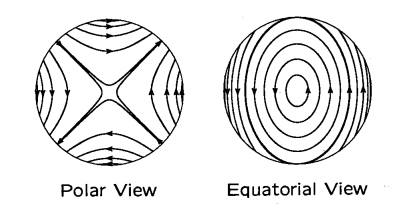
\includegraphics[width=\textwidth]{figure/rmodes.png}
  \end{minipage}
  \hfill
  \begin{minipage}[b]{0.5\textwidth}
    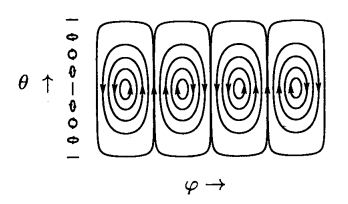
\includegraphics[width=\textwidth]{figure/rmodes1.png}
  \end{minipage}
\caption{Top figure: Top and side view of $l = m = 2$ $r$-mode oscillation.
Bottom figure: The four pattern flows backward with angular velocity $-1/3\Omega$. The
left path shows the motion of individual fluid element that depends on the mode
amplitude. Figure from ~\cite{lindblom2001neutron}.}
\end{figure}
 Viscous mechanism dampens the mode but a mechanism known as
Chandrasekhar-Friedman-Schutz(CFS) instability
~\cite{PhysRevLett.24.611}\cite{1978ApJ...222..281F} drives the R-modes due to
gravitational waves emission. CFS instability can be understood as, on a non
rotating star, gravitational waves releases positive angular momentum from
forward moving mode and negative angular momentum from backward moving mode
damping both modes. For a rotating star, backward moving modes are dragged
forward as viewed from an inertial frame emitting positive angular momentum. But
on rotating frame, modes has negative angular momentum, so the gravitational
waves increases the amplitude of modes instead of damping it. This discrepancy
of modes oscillation between rotating and an inertial frame is known as CFS
instability. This instability causes the amplitude of mode to
grow.~\cite{Owen_2000} 

\section{Viscous damping}
The $r$-modes amplitude grow exponentially and spin down the pulsar abruptly
unless some non-linear mechanism stops the growth~\cite{}. But milliseconds
pulsar exists, that shows $r$-modes saturates at some amplitudes. So, there
needs to be a damping mechanism that saturates the mode amplitude.  The fluid
inside neutron stars are subject to different viscous mechanism damping the
$r$-modes. The viscosity mostly depends on the temperature of the stars.

Shear viscosity has a shorter timescale at lower temperature that can be
calculated by neutron-neutron scattering cross sections~\cite{Owen_2000}. The dissipation
of mode energy is determined by momentum transport and neutrons, protons and
electrons energy present in the neutron star~\cite{1987ApJ...314..234C}. When
the temperature falls below superfluid temperature, the neutron and proton
transforms into superfluid states and doesn't contribute dissipation due to
momentum transport~\cite{1987ApJ...314..234C}. So, only electron-electron
scattering will able to transport momentum during superfluid state. The
dissipation time scale due to shear viscosity from neutron-neutron and
electron-electron scattering are~\cite{ANDERSSON_2001}:
\begin{align*}
t_{sv(nn)}&=\left(\frac{M}{1.4M_\odot}\right)^{-5/4}\left(\frac{R}{10km}\right)^23/4\left(\frac{T}{10^9K}\right)^2\\
t_{sv(ee)}&=\left(\frac{M}{1.4M_\odot}\right)^{-1}\left(\frac{R}{10km}\right)^5\left(\frac{T}{10^9K}\right)^2
\end{align*}
For $n=1$ polytrope star, $t_{sv(nn)}=6.7\times 10^7 s$ and
$t_{sv(ee)}=2.2\times 10^7 s$ . So, neutron star are more viscous in superfluid
state than normal state, which is different from generally known superfluidity
of $He_4$.~\cite{1987ApJ...314..234C}

Bulk viscosity arises from the compression and rarefaction of the fluid that
disturbs the beta equilibrium ($p+e^- \leftrightarrow n +
\nu_e$)~\cite{Owen_2000}. The neutrino carries away the energy from the stars.
Bulk viscosity dominates at higher temperature ($T>10^9 K$) but for $T > 10^{12}
K$, the stars becomes opaque to neutrino. This is because at higher temperature,
the neutrino mean free path length will be less  than the neutron star
radius~\cite{page2013stellar}. So, $r$-modes amplitude might grow
for a new born supernovae and release the rotational energy through
gravitational radiation. At lower temperature there won't be enough thermally
excited nucleons to undergo the Urca process.

The bulk viscosity timescale for n = 1 polytrope is~\cite{ANDERSSON_2001}:
\begin{equation}
t_{bv}=2.4 \times 10^{10}
\left(\frac{M}{1.4M_\odot}\right)^{-1}\left(\frac{R}{10km}\right)^5\left(\frac{T}{10^9K}\right)^{-6}\left(\frac{\nu}{1000 Hz}\right)^2
\end{equation}
So, we can see from above equation, the shear viscosity dissipation decreases
with temperature while the bulk viscosity increases with temperature.

The gravitational radiation makes the mode unstable in rotating stars while
viscosity damps the mode. The $r$-mode growth time scale needs to be fast enough not to be damped by the
viscosity. The $l=m=2$ modes has the shortest timescale and higher multipole has
significantly weaker instabilities~\cite{ANDERSSON_2001}. The timescale of
\ac{GW} radiation of $r$-modes is~\cite{ANDERSSON_2001}:
\begin{equation}
t_{gw}=-47                                                       
\left(\frac{M}{1.4M_\odot}\right)^{-1}\left(\frac{R}{10km}\right)^{-4} \left(\frac{T}{10^9K}\right)^{-6}\left(\frac{\nu}{1000
Hz}\right)^6
\end{equation}
where the negative sign means the mode is unstable.

\section{$r$-mode instability window}
The dissipative timescales can be written as~\cite{Owen_2000}:
\begin{equation}
\frac{1}{t}=-\frac{1}{2E}\frac{dE}{dt}=\frac{1}{t_{gw}}+\sum_v \frac{1}{t_v}
\end{equation}
The mode is stable when $t>0$ and unstable when $t<0$. 
The instability of mode is defined by a critical frequency such that:
$\frac{1}{t_{gw}}+\sum_v \frac{1}{t_v}= 0$
The gravitational radiation timescale depends on the spin frequency and viscous
timescale depends on temperature. 

The width of instability window increases with spin
frequency of neutron star\ref{fig:instability}. On new born supernovae remnants
$r$-modes amplitude grows up exponentially until it reaches a saturation point or
the waves breaks into daughter modes when non-linear hydrodynamic processes
comes in effect~\cite{Owen_1998}. Neutron star are born in a Keplerian limit,
and loose most of the rotational energy due to neutrino cooling.  R-modes might explain the spinning down of old
neutron star into a present low frequency. The evolution of neutron star also
depends on the saturation amplitude and spin frequency the r-modes enters
the instability window~\cite{Alford_2014}. The neutron star with
saturation amplitude($\alpha$)=1 can spin down in 12.3 years with final
temperature of $12.6 \times 10^8 K$ whereas with $\alpha=10^{-4}$ can spin-down a
pulsar in $6.11 \times 10^7$ years with temperature of $2 \times 10^8
K$~\cite{Alford_2014}. Some author claims
$r$-modes saturation amplitude is well below unity and amplitude greater than
unity decays into other fluid modes~\cite{Gressman_2002}. The $r$-mode can split
into daughter mode which amplitude grows exponentially if the parent mode
exceeds certain threshold, where the daughter mode takes energy from parent mode
\cite{Arras_2003}.
\begin{figure}[bht!]                                                            
        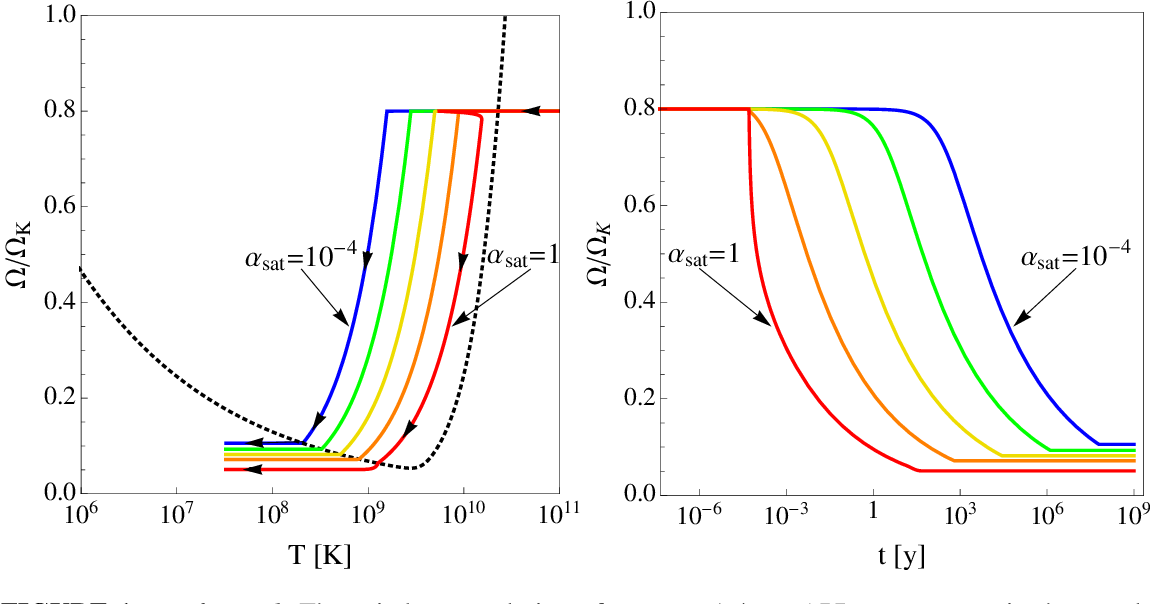
\includegraphics[width=\textwidth]{figure/rmodesamplitude.png}                         
	\caption{Left figure: The spin and temperature  evolution of $1.4 M_\odot$ neutron star
for different saturation amplitude and initial spin frequency entering the
instability window. The dotted curve shows the instability window. Right figure: The spin evolution with respect to time. Figure from ~\cite{Alford_2014}}
        \label{fig:instability}                                                     
\end{figure}  






\section{R-modes frequency}
The neutron stars interior are composed of neutron rich ocean. In a rotating
star, the liquid surface are subject to a Coriolis force similar to the Rossby
waves. These non-radial oscillation known as $r$-modes are unstable to the
gravitational radiation. They might live for a long time even in the presence of
viscosity.
The harmonic time dependent displacement vector of mode propagating in azimuthal
direction can be written as~\cite{ANDERSSON_2001}:
\begin{equation}\label{modesvector}
\vec{\xi}= \vec{\xi} e^{i(m\varphi+\omega_r t)}
\end{equation}
where m is the magnetic moment, $\omega_r$ is the oscillation of modes in
rotating frame.
The inertial frame are related to rotating frame by the equation:
\begin{equation}\label{inertialconvt}
\left(\frac{d}{dt}\right)_i=\left(\frac{\partial}{\partial t}\right)_r+\vec{u}.\nabla=\partial_t+ \Omega
\partial_\varphi
\end{equation}
Plugging \ref{modesvector} in \ref{inertialconvt}, we get,
\begin{equation}
\omega_i=\omega_r - m\Omega
\end{equation}

The frequency of modes in rotating frame is:
\begin{equation}\label{rotatingframe}
\omega_r = \frac{2m\Omega}{l(l+1)}
\end{equation}

The dominant $r$-mode is with spherical harmonic (l=m=2). The other mode has
weaker instability, the growth time of instability increases by a magnitude
with increase of l~\cite{ANDERSSON_2001}.
So, $\omega=2/3\Omega$, and plugging this into \ref{inertialconvt},
$\omega_i = -4/3\Omega$
The negative sign is the discrepancy of mode as seen in the rotating and
inertial frame and this discrepancy causes the modes amplitude to grow instead
of damping from gravitational radiation. 

\subsection{Factors affecting $r$-mode frequency}
The $r$-mode frequency will deviate from the Newtonian case when relativistic
error are considered. 


\subsubsection{General Relativity}
The $r$-mode frequency are dependent on a compactness of star which is the ratio
of mass over radius($M/R$).The compactness can be parametrized as:
\begin{equation}\label{compactness}
\frac{M}{R}=\left(\frac{M}{1.4M_\odot}\right)\left(\frac{10km}{R}\right)\left(\frac{1.4M_\odot}{10^4m}\right)
\end{equation} 
One solar mass in geometrized units(c=G=1) is equal to 1474. So, plugging the
numbers in \ref{compactness} gives:
\begin{equation}
\frac{M}{R}=0.21\left(\frac{M}{1.4M_\odot}\right)\left(\frac{10km}{R}\right)
\end{equation} 
The maximum compactness is given by~\cite{LATTIMER_2007}:
\begin{equation}
R \geq 2.83GM/c^2
\end{equation}
In geometrized units, the above equation will be $M/R \leq 0.35$
\citet{LATTIMER_2007} gives the probable minimum mass of neutron
star($1_M\odot$) will have radius of 14.5 km, making $M/R=0.103$.
\citet{Idrisy_2015} gives a conservative limit of compactness, $0.11 \leq M/R
\leq 0.31$. They have used the lowest mass as $1.02M_\odot$ and maximum mass of
neutron star as $2.76M_\odot$. The frequency of $r$-modes in relation to
compactness($M/R$) and spin frequency($\nu$) is~\cite{Idrisy_2015}: 
\begin{equation}
f=(-1.379 + 0.079(M/R) - 2.25(M/R)^2)*\nu
\end{equation}  
Plugging in the range of compactness (0.11-0.31), the $r$-mode frequency,
$f=(1.39-1.57)\nu$
The effect of general relativity will increase the $r$-mode frequency in an
inertial frame by few percentage.

\subsubsection{Rapid rotation}
The second order correction is important for a rapidly rotating neutron stars.
On, Newtonian star, the second order formula for $r$-mode frequency is given by 
\cite{Lindblom_1999}.
\begin{equation}
f/\nu=\kappa_0 - 2 + \kappa_2 \Omega^2/\pi G \rho_0
\end{equation}
where $\kappa_0=\sigma_I/\Omega$, $\kappa_2$ is a dimensionless parameter,
$\rho$ is a average mass density.
As $\kappa_0=2/3$, the above equation is:
\begin{equation}
f/\nu = -4/3 + \kappa_2 \Omega^2/\pi G \rho_0
\end{equation}

\begin{equation}
\frac{\Omega^2}{\pi G \rho_0}=0.145 \left(\frac{\nu}{716 Hz}\right)^2
\left(\frac{R}{10km}\right)^3 \left(\frac{1.4M_\odot}{M}\right)
\end{equation}

For the Crab with spin frequency $29.6 Hz$, taking mass and radius as
$1.4M_\odot$ and 12.53 km, and $\kappa_2 = 0.29$~\cite{Lindblom_1999} , the
rotational correction  will change $r$-mode frequency by 0.01\%. The correction
will be around 8\% for a fastest rotating neutron star. So, the rapidly rotation
correction will be less than the general relativity correction but it can be
significant for a pulsar rotating near mass shedding limit.

\subsubsection{Crust core coupling}
The crust are formed when neutron star cools off to temperature below
$10^{10}K$.  The friction between neutron fluids and the solid crust can dampen
the $r$-mode.  If the $r$-amplitude is high enough it can heat the crust-core
interface~\cite{Lindblom_2000}. The thermal heating can also lose in thermal
conduction and neutrino emission on core-crust boundary. The elastic storing
force on crust is less than the Coriolis force, so for a fast rotating neutron
star the crust will oscillate like a liquid with low shear
modulus~\cite{Levin_2001}. When the spin frequency increases, the $r$-mode
frequency will rise to meet the elastic crust modes causing avoided
crossing~\cite{Levin_2001}. The departure from the $r$-mode frequency in rotating
frame ($\omega_r=2/3\Omega$) is significant for spin frequency interval
$0.05\leq\Omega/\Omega_k\leq0.1$~\cite{Idrisy_2015}. The avoided crossing is
similar to the mode splitting in coupled pendulum by varying the length of one
pendulum. 

\subsection{$r$-mode frequency parameter after relativistic correction}
On \cite{Yoshida:2004gk} , the $r$-mode frequency is written in terms of correction due to the
compactness and rapid rotation. And, $r$-mode frequency is a decreasing function
of $T/|W|$, where $T/|W|$ is the ratio of rotational energy to the gravitational
binding energy. 
\begin{equation}\label{eq:T/W}
\frac{f}{\nu}=(1.41 - 1.50) - (1.23-1.95)T/|W|
\end{equation}	
The relativistic correction (1.41 - 1.50) are more precisely calculated to (1.39
- 1.57)~\cite{Idrisy_2015}. For, a mass shedding of 0.1,the equation ~\ref{eq:T/W} can be written as :
\begin{equation}
\frac{f}{\nu}=(1.39 - 1.57) - (0-0.195)\frac{\nu}{\nu_k^2}
\end{equation}	
where $\nu_k$ is the Keplerian velocity. The lower limit of the second order
correction of $r$-mode frequency is not known, so we choose it to zero. The
correct parameter of $r$-mode frequency will be discuss in details in the next
chapter. 
%%%%%%%%%%%%%%%%%%%%%%%%%%%%%%%%%%%%%%%%%%%%%%%%%%%%%%%%%%%%%%%%%%%%%%%%%%%%%%%%%%%%%%%%%
%%%%%%%%%%%%%%%%%%%%%%%%%%%%%%%%%%%%%%%%%%%%%%%%%%%%%%%%%%%%%%%%%%%%%%%%%%%%%%%%%%%%%%%%%
%%% 							END OF THIRD CHAPTER								  %%%
%%%%%%%%%%%%%%%%%%%%%%%%%%%%%%%%%%%%%%%%%%%%%%%%%%%%%%%%%%%%%%%%%%%%%%%%%%%%%%%%%%%%%%%%%
%%%%%%%%%%%%%%%%%%%%%%%%%%%%%%%%%%%%%%%%%%%%%%%%%%%%%%%%%%%%%%%%%%%%%%%%%%%%%%%%%%%%%%%%%

\chapter{How to search for gravitational waves from $r$-modes of known pulsars}
\section{Introduction}

In terms of strain, the most sensitive searches for \acp{GW} are those for
continuous waves, signals emitted by spinning neutron stars which need not be
in binaries.
The most sensitive searches for continuous \acp{GW} are those for known
pulsars, for which a timing solution derived from \ac{EM} observations
allows coherent integration of years of data~\cite[and references
therein]{Riles:2017evm}.
Most known pulsar searches (most recently~\cite{Authors:2019ztc}) have
targeted \ac{GW} frequencies precisely double (or occasionally equal to) the
observed spin frequency of each pulsar, based on electromagnetic pulse timing
and assuming an emission model of a ``mountain''---a mass quadrupole rotating
with the star.
Some known pulsar searches (most recently~\cite{Abbott:2019bed}) have instead
targeted narrow frequency bands of a fraction of a~Hz, losing some sensitivity
and costing more than fully targeted search, but allowing for some
uncertainties in the \ac{EM} timing parameters and in the physics such as the
possibility of free precession.

Neutron stars might also emit \acp{GW} via $r$-modes, rotation-dominated
quasi-normal modes driven unstable by gravitational radiation with frequencies
roughly 4/3 the spin frequency of the star~\cite[and references
therein]{Paschalidis:2016vmz}.
There are many uncertainties in the damping mechanisms that compete with the
instability and in the amplitudes attainable by $r$-modes due to nonlinear
hydrodynamics and other saturation mechanisms.
Within those uncertainties, $r$-modes might be oscillating at relatively low
amplitudes in fast spinning young pulsars up to several thousand years after
their birth, in rapidly accreting neutron stars, and in millisecond pulsars
perhaps a long time after accretion stops~\cite[and references
therein]{Glampedakis:2017nqy}.

So far \ac{GW} searches have only set upper limits on $r$-modes in broad band
(hundreds to thousands of~Hz) searches for non-pulsing neutron stars (most
recently~\cite{Abbott:2018qee}), but searches could be done for $r$-modes from
known pulsars too.
The main issue is determining the frequency band to search.
The uncertainty in $r$-mode frequency for a known pulsar is typically a
few~Hz~\cite{Idrisy:2014qca}, broader than previous narrow band pulsar
searches but not as broad as previous $r$-mode searches.
For long integrations, which are the most sensitive searches, some thought
needs to be given to spin-down parameters as well.

The main caveat is that $r$-modes might not truly be unstable (damping might
beat driving) in all or most neutron stars once all damping mechanisms are
taken into account.
Another caveat is that $r$-modes might be unstable but saturate at amplitudes
too small to be detectable with present and near-future detectors.
Predictions of saturation amplitudes~\cite{Arras:2002dw} are indeed too small
to detect for most pulsars and present detectors~\cite{Owen:2010ng}.
But calculations of saturation amplitude might be wrong and \ac{GW} detectors
are improving.
Also, it takes some time to develop and refine a \ac{GW} search, so it is
worthwhile to start now.

In this article we describe how to perform searches for \acp{GW} from
$r$-modes of known pulsars using minimal adaptations of existing code.
In particular the directed search pipeline used most recently in
Ref.~\cite{Abbott:2018qee}, based on the implementation of the
$\mathcal{F}$-statistic in LALSuite~\cite{LALSuite}, is easily adaptable for
this purpose.
We present a method for choosing a search parameter space and estimate
computational costs and sensitivities using that method.
(The parameter space was partially estimated once before~\cite{Ian}.)
We show that interesting searches of data from LIGO's \ac{O1} and \ac{O2} are
feasible already, and that future searches of more sensitive data sets will be
even more interesting.
Along the way we highlight the main issues affecting realistic observations,
which leads naturally to a list of suggestions for future work both by
theorists and by data analysts.

\section{Assumptions}

\subsection{Physics}

We assume that the \ac{GW} frequency evolution $f(t)$ in the reference frame
of the solar system barycenter is
\begin{equation}
\label{ft}
f(t) = f\left( t_0 \right) + \dot f\left( t_0 \right) \left( t-t_0 \right) +
\frac{1}{2} \ddot f\left( t_0 \right) \left( t-t_0 \right)^2,
\end{equation}
where $t_0$ is some reference time (often the beginning of the observation),
dots indicate time derivatives, and we shall use a simple $f$ to indicate
$f(t_0)$ from now on.
Physically, Eq.~(\ref{ft}) assumes that the signal frequency does not change
too fast (such as from glitches or higher derivatives) or too erratically
(such as from timing noise).
Timing noise is unlikely to be an issue for the integration times (a year or
less) considered here~\cite{Ashton:2014qya}.
Glitches can be avoided by checking \ac{EM} observations.
As we shall see below, higher derivatives are not a problem, and for some
searches even the second derivative is not needed.

Throughout we consider the lowest order (current quadrupole) $r$-mode, since
it is the fastest driven by \ac{GW} emission and the least damped by most
forms of viscosity.

We shall make frequent use of the ``spin-down limits''~\cite{Owen:2010ng} on
intrinsic \ac{GW} strain~\cite{Jaranowski:1998qm}
\begin{equation}
h_0^\mathrm{sd} \simeq 1.6\times10^{-24} \left( \frac{\mbox{1 kpc}}{r} \right)
\left( \frac{\left|\dot f\right|} {10^{-10}\mbox{ Hz/s}} \frac{\mbox{100 Hz}}
{f} \right)^{1/2}
\label{h0sd}
\end{equation}
(where $r$ is the distance to the pulsar) and on the $r$-mode amplitude
parameter~\cite{LMoO:1998prl}
\begin{equation}
\alpha_\mathrm{sd} \simeq 0.033 \left( \frac{\mbox{100 Hz}} {f} \right)^{7/2}
\left( \frac{|\dot{f}|} {10^{-10}\mbox{ Hz\,s}^{-1}} \right)^{1/2}.
\end{equation}
These correspond to the assumption that all of the observed $\dot f$ is due to
\ac{GW} emission via $r$-modes.
That is clearly an unrealistic assumption, especially when considering the
observed values of second derivatives too; but these limits serve as useful
milestones for search sensitivity.
These numerical forms of the limits assume certain neutron star structure
parameters and also assume that the ratio of \ac{GW} frequency to spin
frequency is 4/3, so they are uncertain by a factor of two or
so~\cite{Owen:2010ng}.
While they should not be taken too literally, these spin-down limits give a
rough idea of which \ac{GW} searches are most interesting.

There are many debates on the growth and damping timescales of the $r$-modes,
and on the saturation amplitude (which determines the long term strength of
\ac{GW} emission).
We largely bypass them, though we note that $\alpha$ is predicted to saturate
at order $10^{-4}$ or lower~\cite{Arras:2002dw}.
Theoretical uncertainties in these quantities are great and might best be
resolved by observations which do not rely too much on theoretical guidance to
pick targets.
Attempts at relatively model independent predictions or connections to
electromagnetic observations sometimes favor or disfavor one pulsar or
another.
Alford and Schwenzer~\cite{Alford:2012yn} argue that $r$-modes in young
neutron stars spinning down shut off above 60~Hz under a wide variety of
conditions, making PSR~J0537\textminus6910 the best candidate.
They also propose that the braking index (see below) could be as low as four
in some $r$-mode dominated pulsars rather than seven as implied for
constant~$\alpha$ evolution~\cite{Owen:1998xg}.
Certainly J0537\textminus6910 has the best (lowest)
$\alpha_\mathrm{sd}$ for all young pulsars~\cite{Owen:2010ng} (order
$10^{-1}$), and there are hints that the braking index between its frequent
glitches might be seven~\cite{Andersson:2017fow}.
There are also arguments that millisecond pulsars will emit \acp{GW} from
$r$-modes for a long time, but only at small amplitudes even if they have high
spin-down limits~\cite{Bondarescu:2013xwa, Alford:2014pxa}.
And temperature observations of some pulsars might indicate small $r$-mode
amplitudes due to constraints on viscous heating~\cite{Schwenzer:2016tkf}.
But as observers we note that the universe holds many surprises, and we
consider searches for any pulsar with an attainable spin-down limit.

An $r$-mode emits \acp{GW} at the mode's oscillation frequency $f$ in an
inertial frame of reference.
This frequency is a function of star's spin frequency $\nu$ of the
form~\cite[e.g.]{Yoshida:2004gk}
\begin{equation}
\label{fnu}
f/\nu = A - B \left( \nu / \nu_K \right)^2 + O(\nu)^4,
\end{equation}
where we have chosen the signs so that $A>0$ and $B>0.$
(The sign of the second term is generic to retrograde modes, such as all
$r$-modes, and is due to the effects of gravitational redshift and dragging of
inertial frames on the Coriolis force~\cite{Paschalidis:2016vmz}.)
Both parameters depend on the (usually unknown) mass $M$ and radius $R$ of the
neutron star and the still uncertain equation of state, and both are
dimensionless numbers of order unity.
The rapid rotation calculation of $r$-mode frequencies in
Ref.~\cite{Yoshida:2004gk} indicates that the $O(\nu)^4$ remainder in
Eq.~(\ref{fnu}) is negligible except (for some stars) when the star is
spinning almost at its Kepler frequency $\nu_K,$ the frequency at which
centrifugal force tears it apart.
Most pulsars, including those we find most interesting for this analysis, spin
at much less than the 716~Hz of the fastest observed
frequency~\cite{Manchester:2004bp}, so we will neglect the $O(\nu)^4$
remainder in Eq.~(\ref{fnu}).
We also assume that any backbending (nonmonotonic $f$ vs.\ $\nu$) due to a
possible phase transition~\cite{Glendenning:1997fy} occurs at much higher
frequencies and does not appreciably affect Eq.~(\ref{fnu}).

In Eq.~(\ref{fnu}) we neglect many physical effects which should have only a
small effect on the ranges of $A$ and $B.$
We assume that any differential rotation has a negligible effect on the mode
frequency.
In practice this seems likely to be true, even though the $r$-mode tends to
generate a small amount of differential rotation analogous to Stokes
drift~\cite{Friedman:2017wfi}.
We assume that the magnetic field's direct effect (through restoring force) on
the $r$-mode frequency is small.
Several studies (most recently~\cite{Jasiulek:2016epr}) indicate that this is
true for the relatively low magnetic fields of pulsars spinning in the LIGO
band.
While superfluidity generally has only a tiny effect on the mode
frequencies~\cite{Lindblom:1999wi}, it does split each normal fluid $r$-mode
into two where the neutron and proton fluids are co-moving or
counter-moving~\cite{Andersson:2001bz}; and the latter mode has an additional
restoring force due to entrainment of the two fluids.
These modes in general have slightly different frequencies, but the
counter-moving modes tend to be much more damped by mutual friction.
Thus we can assume that the \ac{GW} emission is almost all through co-moving
modes, which have frequencies almost identical to normal fluid modes.

More serious is the issue of avoided crossings between $r$-modes and other
modes.
For example, Levin and Ushomirsky~\cite{Levin:2000vq} pointed out that, as a
star spins down, the $r$-mode and a torsional mode of the solid crust
(vibrating at of order 100~Hz in a nonrotating star) will swap identities.
More sophisticated calculations~\cite[e.g.]{Glampedakis:2006ap} support this
idea.
A similar issue arises with the coupling between the $r$-modes and the buoyant
force responsible for $g$-modes~\cite{Kantor:2017xuo}.
In either case, in the vicinity of the other mode's frequency the avoided
crossing introduces large errors into the simple $r$-mode frequency dependence
posited in Eq.~(\ref{fnu}).
We shall neglect this, and assume that the pulsars we consider have $\nu$
safely away from the major avoided crossings.
In a search for many pulsars, most of them are likely to satisfy this
assumption; but it is a potentially serious issue worthy of more research.

The other potentially major effect is the coherence time of the $r$-modes.
If mode-mode coupling calculations such as Ref.~\cite{Brink:2004kt} are
correct, a saturated $r$-mode exists in rough equilibrium with two ``daughter
modes'' but may occasionally undergo abrupt phase shifts~\cite{Ira}.
A similar situation could hold if one attempts to take advantage of the
relatively broad band of frequencies to search for $r$-modes from a pulsar
which does not have \ac{EM} timing contemporary with a \ac{GW} data run---the
pulsar could have glitched during the \ac{GW} run, introducing a phase error
at a random time.
Such phase errors would reduce the sensitivity of coherent data analysis
methods described below~\cite{Ashton:2017wui}.

\subsection{Data analysis}

We assume a search method based on coherent integration using a minimal
adaptation of the code used in several broad band directed searches, most
recently Ref.~\cite{Abbott:2018qee}.
This code implements the multi-interferometer
$\mathcal{F}$-statistic~\cite{Jaranowski:1998qm, Cutler:2005hc}, which
combines matched filters in such a way as to account for the daily changes of
the interferometers' beam patterns as the Earth rotates.
This particular code implements the ``demodulated'' $\mathcal{F}$-statistic
first used in Ref.~\cite{Abbott:2003yq}.
A ``resampled'' implementation of the
$\mathcal{F}$-statistic~\cite{Patel:2009qe} could speed up computations
considerably, although it would present some difficulties in dividing up the
parameter space.
The $\mathcal{F}$-statistic also quickly maximizes signal-to-noise ratio over
the (typically unknown) angles describing the orientation of the neutron
star's spin axis.
In Gaussian noise, $2\mathcal{F}$ is drawn from a $\chi^2$ distribution with
four degrees of freedom.
In the presence of a signal, the $\chi^2$ is noncentral and the power
signal-to-noise ratio (if large) is approximately $\mathcal{F}/2.$

For some pulsars a wind nebula indicates the orientation of the star's spin
axis, and in that case a similar statistic called the
$\mathcal{G}$-statistic~\cite{Jaranowski:2010rn} can achieve slightly better
sensitivity.
Since the $\mathcal{G}$-statistic is not included in the implementation of the
$\mathcal{F}$-statistic in LALSuite~\cite{LALSuite} used in
Ref.~\cite{Abbott:2018qee}, we do not consider it further here; but it is a
natural avenue of future improvement.

We assume that the \ac{GW} search can use a single sky position.
Pulsar positions are typically known to sub-arcsecond
precision~\cite{Manchester:2004bp} and the sky resolution of a directed
continuous \ac{GW} search is two orders of magnitude less precise at the
frequencies of most pulsars~\cite[e.g.]{Abbott:2018qee}.

We do not assume we have a coherent \ac{EM} pulsar timing solution throughout
the \ac{GW} observation.
Narrow band searches for pulsars such as~\cite{Abbott:2019bed} are already
broad enough to extrapolate \ac{EM} timing from old observations, and since
our search bands turn out to be broader they are even more robust.
The main worry is whether there is a glitch during the \ac{GW} observation, in
which case it will effectively cut the integration time and reduce the
signal-to-noise ratio~\cite{Ashton:2017wui}.

We do assume that, in cases where the pulsar is a component of a binary, the
binary's orbital parameters are known well enough to avoid requiring a search
over them.
This is true for most binary pulsars except those in low mass x-ray binaries.
Since those are accreting and therefore the spin can undergo random walks, we
neglect them for our present purposes.

\section{Parameter space}

Under the assumptions stated above, the parameter space of a search consists
of ranges of $f,$ $\dot f,$ and possibly $\ddot f.$
With some uncertainties, these can be calculated as functions of the
\ac{EM}-observed spin $\nu$ and spin-down parameters $\dot\nu$ and $\ddot\nu.$

\subsection{General expressions}

Assuming that $A$ and $B$ do not change appreciably with time, the time
derivatives of Eq.~(\ref{fnu}) yield
\begin{eqnarray}
\label{fdot}
\dot f / \dot \nu &=& A - 3B \left( \nu/\nu_K \right)^2,
\\
\label{fddot}
\ddot f / \ddot \nu &=& A - \left( 3 + 6/n \right) B \left( \nu/\nu_K
\right)^2,
\end{eqnarray}
where $n = \nu \ddot \nu / \dot \nu^2$ is the braking index of the pulsar.
Thus an observation of $(\nu, \dot\nu, \ddot\nu)$ and calculations of $\nu_K$
and the ranges of $(A,B)$ determine the ranges of $(f, \dot f, \ddot f)$ to be
searched---in principle.
In practice $\ddot\nu$ tends to have significant uncertainties, affecting the
choice of $\ddot f$ as discussed below.

To get the frequency range of a search we insert the ranges of $A$ and $B$
into Eq.~(\ref{fnu}) and---for now---assume that $\nu_K$ is known to obtain
\begin{eqnarray}
(f/\nu)_{\min} &=& A_{\min} - B_{\max} \left( \nu/\nu_K \right)^2,
\\
(f/\nu)_{\max} &=& A_{\max} - B_{\min} \left( \nu/\nu_K \right)^2.
\end{eqnarray}

To determine the range of $\dot{f}$ for a given $f,$ note that
Eqs.~(\ref{fnu}) and~(\ref{fdot}) can be combined to write
\begin{equation}
\dot f / \dot \nu = f / \nu - 2B \left( \nu/\nu_K \right)^2.
\end{equation}
Then we simply have the range
\begin{eqnarray}
\left( \dot{f} / \dot\nu \right)_{\min} &=& f / \nu - 2B_{\max} \left(
\nu/\nu_K \right)^2,
\\
\left( \dot{f} / \dot\nu \right)_{\max} &=& f / \nu - 2B_{\min} \left(
\nu/\nu_K \right)^2.
\end{eqnarray}

Note that Eqs.~(\ref{fnu}) and~(\ref{fdot}) combined determine $A$ and
$B/\nu_K^2$ as
\begin{eqnarray}
A &=& \left( 3f / \nu - \dot{f} / \dot{\nu} \right) /2,
\\
B/\nu_K^2 &=& \left( f / \nu - \dot{f} / \dot{\nu} \right) / \left( 2\nu^2
\right).
\end{eqnarray}
These relations can be used for parameter estimation from a \ac{GW} detection:
Once $f$ and $\dot f$ are known, we find $A$ and $B/\nu_K^2,$ which in turn
can yield information on $M$ and $R$ and the equation of
state~\cite{Yoshida:2004gk, Idrisy:2014qca}.
The equations for $A$ and $B$ also can be used to write
\begin{equation}
\ddot{f} / \ddot{\nu} = \dot{f} / \dot{\nu} - (3/n) \left( f / \nu - \dot{f} /
\dot{\nu} \right),
\end{equation}
which in principle uniquely determines $\ddot f$ in terms of $f,$ $\dot f,$
and \ac{EM}-observed quantities.

In practice, $\ddot\nu$ (or equivalently $n$) measurements are available only
for a few pulsars; and even then they may have large errors when measured over
short baselines.
For example, the monthly fits to $\ddot\nu$ for the Crab pulsar provided by
Jodrell Bank can vary by a factor of a few from the long term average and can
even change sign~\cite{Crab2015}.
It is not clear how much of this timing noise is due to magnetospheric effects
and how much is due to a genuine fluctuating torque on the star.
Since the $r$-mode frequency is determined mainly by the Coriolis force, we
are interested in the latter but not the former.
However at the moment we wish to be cautious in our choice of parameter space.
As a practical matter, current codes including that used in
Ref.~\cite{Abbott:2018qee} cut the parameter space into computing batch jobs
in a way such that the range of $\ddot f$ can depend on $f$ but not on $\dot
f.$
Plugging in the full range of $\dot f$ we can get
\begin{eqnarray}
\left( \ddot f / \ddot\nu \right)_{\min} &=& f/\nu - 2(1+3/n) B_{\max} \left(
\nu/\nu_K \right)^2,
\\
\left( \ddot f / \ddot\nu \right)_{\max} &=& f/\nu - 2(1+3/n) B_{\min} \left(
\nu/\nu_K \right)^2
\end{eqnarray}
as functions of $f.$
To err on the safe side by covering more parameter space, we can take the
minimum $\ddot f$ as zero.
Since our ``safe side'' $B_{\min}$ vanishes (see below), the maximum $\ddot f$
can be taken to be simply $\ddot\nu f/\nu,$ using the highest $\ddot\nu$
observed during the \ac{GW} integration.

At the moment these overly broad parameter ranges are not a concern, because
\ac{O1} searches are computationally cheap and even \ac{O2} searches are not
extravagant (see below).
These parameter ranges could be refined later for longer searches, when
computational cost is more of an issue, for example by calculating the range
of $B$ and exploring its consequences.

\subsection{Numerical ranges of parameters}

The range of $A$ is fairly well known.
The most recent calculation~\cite{Idrisy:2014qca} used the general
relativistic slow rotation approximation~\cite{Lockitch:2000aa,
Lockitch:2002sy} to compute $A$ for a variety of neutron-star equations of
state, obtaining 1.39 $\le A \le$ 1.57 depending almost purely on $M/R.$
Since that calculation was published, the big new constraint on the neutron
star equation of state is the lack of a large tidal effect in the binary
neutron-star merger GW170817~\cite{TheLIGOScientific:2017qsa}.
This disfavors large radii and low $A.$
But for the rest of this paper, to be conservative (cover a wide range of
parameters), we shall use the $A_{\min}$ and $A_{\max}$ quoted above.

The range of $B$ is less well known than the range of $A.$
The best general relativistic calculation~\cite{Yoshida:2004gk} drops the slow
rotation approximation, but adds the Cowling approximation (neglecting the
metric perturbation) and gives numbers only for two equations of state and two
$M/R$ values.
And the equations of state are polytropes rather than realistic equations of
state with the adiabatic index varying depending on the density.
The errors due to the Cowling approximation can be estimated as a few percent,
which is not of too much concern here; but the uncertainty from the stellar
models is more serious.

We estimate the range of $B$ from Ref.~\cite{Yoshida:2004gk} as follows:
Their Eq.~(15) gives $B\left( \nu/\nu_K \right)^2$ as 1.23--1.95 times the
ratio of kinetic to potential energy for the four stellar models considered.
For our purposes the most interesting model is their model $c,$ a polytrope of
adiabatic index~2 and $M/R=0.1$ which yields the number 1.95 (and for which
the slow rotation approximation is very accurate all the way to the Kepler
frequency).
In Fig.~2 of Ref.~\cite{Yoshida:2004gk} the sequence for model $c$ terminates
at a kinetic-to-potential energy ratio of 0.1, and this termination point
corresponds to $\nu=\nu_K,$ the ``Kepler frequency'' or maximum spin frequency
of the star.

Hence we can write $B \simeq 0.195$ for this stellar model, which should set a
safe upper limit on $B_{\max}$ for the following reasons:
The results of Ref.~\cite{Yoshida:2004gk} show that $B$ increases for smaller
$M/R$ and for lower adiabatic index (higher polytropic index).
The value $M/R=0.1$ for their model $c$ is smaller than post-GW170817 bounds,
indicating we are safe there.
An adiabatic index of~2 also errs on the safe side, since piecewise polytropic
fits to realistic equations of state~\cite{Read:2008iy} yield higher indices.
The bound on $B_{\min}$ is less clear without detailed calculations, but
$B_{\min}=0$ is well beyond the range quoted and should be safe.

Last we consider $\nu_K.$
The fastest observed spin frequency for a neutron star is about
716~Hz~\cite[and references therein]{Paschalidis:2016vmz}.
The Kepler frequency is expected to scale roughly as its Newtonian dependence
$M^{1/2} R^{-3/2},$ even in general relativity~\cite[and references
therein]{Paschalidis:2016vmz}.
Neutron star radii are roughly constant for a given equation of state, while
reliable mass measurements range over almost a factor of
two~\cite[and references therein]{Ozel:2016oaf}.
To err on the safe side (high $B_{\max}$), we assume that the 716~Hz pulsar is
on the high end of the mass range and our pulsar is on the low end so that it
has a lower Kepler frequency.
Then we can safely take $\nu_K = \mbox{716 Hz}/\sqrt{2} \simeq 506$~Hz, erring
on the safe side by assuming a possible factor of two difference in mass.

To summarize, we recommend for the moment a broad parameter space with ranges
\begin{eqnarray}
\label{range0}
f_{\min} = \nu \left( A_{\min} - B_{\max} \frac{\nu^2} {\nu_K^2} \right),
&\quad&
f_{\max} = \nu\, A_{\max},
\\
\label{range1}
\dot f_{\min} = -\dot\nu \left( \frac{f}{\nu} - 2B_{\max} \frac{\nu^2}
{\nu_K^2} \right),
&\quad&
\dot f_{\max} = -\dot\nu \frac{f}{\nu},
\\
\label{range2}
\ddot f_{\min} = 0,
&\quad&
\ddot f_{\max} = \ddot\nu \frac{f}{\nu},
\end{eqnarray}
where $\ddot\nu$ is the maximum value consistent with \ac{EM} observations,
and the other parameters are $A_{\min} = 1.39,$ $A_{\max} = 1.57,$ $B_{\max} =
0.195,$ and $\nu_K = 506$~Hz.

\section{Computational cost}

We rely heavily on the search parameter space metric~\cite{Wette:2008hg}
\begin{equation}
g_{ij} = \pi^2 \left(
\begin{array}{ccc}
T^2/3 & T^3/6 & T^4/20 \\
T^3/6 & 4T^4/45 & T^5/36 \\
T^4/20 & T^5/36 & T^6/112
\end{array}
\right)
\end{equation}
where the indices are labeled in the order $(f, \dot f, \ddot f)$ and also can
be labeled 0, 1, 2.
Here $T$ is the time from beginning to end of the integration.
This metric controls the density and placement of templates (parameter values
of matched filters) by relating coordinate distances (parameter differences)
to loss of signal-to-noise ratio~\cite{Owen_1996}.
The mismatch $g_{ij} \Delta \lambda^i \Delta \lambda^j$ between two signals
with parameters displaced by $\Delta \lambda^i$ is the fractional loss in
optimal power signal-to-noise ratio due to filtering one with the parameters
of the other.
In continuous \ac{GW} searches template banks are often constructed so that
the worst case mismatch between any signal and the nearest template is 0.2.
We calculate metric components neglecting the amplitude modulation of the
$\mathcal{F}$-statistic and including only phase terms, an approximation which
works well for integrations of many days~\cite{Prix:2006wm}.

To determine which pulsars require $\ddot f,$ we compute $g_{22} \ddot
f_{\max}^2$ to determine the maximum mismatch due to neglecting $\ddot f.$
(Note that this does not allow for the possible mitigating effect of varying
$f$ and $\dot f$ somewhat, and thus it is a conservative estimate.)
If the mismatch is comparable to or greater than 0.2, $\ddot f$ is needed.
First we evaluate this criterion using $\ddot\nu$ values taken from the ATNF
catalogue~\cite{Manchester:2004bp}.
In many cases these values are unknown or are known to be contaminated by
timing noise (such as when they are negative).
However the values of $\nu$ and $\dot\nu$ are typically well measured.
Hence we also check the need for $\ddot f$ using $\ddot\nu = 7 \dot\nu^2 /
\nu$ (implied by a braking index of 7), and if either this mismatch or the one
using the observed $\ddot\nu$ satisfies the criterion we consider a search
over $\ddot f$ to be necessary.

We consider three values of $T:$
First $1.12\times10^7$~s and $2.32\times10^7$~s, the lengths of \ac{O1} and
\ac{O2} respectively, then one year or $3.15\times10^7$~s which might be
characteristic of future LIGO runs~\cite{Aasi:2013wya}.
We only consider pulsars with $f_{\max}$ greater than 10~Hz since, even at
design sensitivity, LIGO noise increases rapidly below that frequency and the
$r$-mode amplitudes required to emit at the spin-down limit become enormous.
We find that for \ac{O1} the Crab, Vela, and several others need $\ddot f;$
while for \ac{O2} and a one-year integration most pulsars with measured
$\ddot\nu$ and several without it need $\ddot f.$

We test the need of the third frequency derivative using $g_{33} = \pi^2 T^8 /
2025$~\cite{Wette:2008hg}, the third derivative of $\nu$ from the ATNF
catalogue~\cite{Manchester:2004bp} when it is given, and the $n=7$ value of
$91 \dot\nu^3 / \nu^2$ for the third derivative when it is not given.
(The numerical factor 91 is $n(2n-1)$ in general, and can be obtained by
differentiating the definition of the braking index.)
For \ac{O1} no pulsar needs a third derivative.
For \ac{O2} no pulsar with a spin-down limit above the noise (see below) needs
a third derivative.
For a one year integration the Crab (alone of the pulsars detectable at the
spin-down limit) is on the edge of needing a third derivative.
Since this is a conservative estimate and the need can be mitigated by
slightly shortening $T$ and our focus here is on how to adapt current data
analysis codes, which do not include the third derivative, we do not address
third derivatives further here.

Under the assumption that two frequency derivatives are needed and three are
not, the proper volume of the parameter space $\sqrt{g} \int df\, d\dot f\,
d\ddot f$ integrated over the ranges in Eq.~(\ref{range0})--(\ref{range2}) is
approximately
\begin{equation}
\label{propvol}
\sqrt{g} \nu \left| \dot\nu \right| \ddot\nu B_{\max} \left( \nu/\nu_K
\right)^2 \left[ A_{\max}^2 - A_{\min}^2 \right].
\end{equation}
(Here we have dropped the $B$ terms in $f_{\min}$ and $f_{\max},$ since they
are small corrections, and $g$ indicates the determinant of the metric.)
To estimate the number of templates, we divide by the proper volume per
template~\cite{Owen_1996},
\begin{equation}
V = \left( 2 \sqrt{\mu/3} \right)^3 \simeq 0.138
\end{equation}
for a three-dimensional template bank mismatch $\mu$ of 0.2.
In cases where $\ddot f$ is not needed, these expressions need to be modified,
but those cases are so computationally cheap that they are not an issue.
In practice the number of templates is modified from these estimates by the
vagaries of the actual template placement code, typically dominated by the
problem of covering the edges of long narrow stretches of parameter space.
Our tests with LALSuite~\cite{LALSuite} show that a real search might use
three times as many templates as these ideal numbers.
Since this factor can vary for each search, we do not include it further or
attempt to estimate the numbers too precisely.

To get values for the number of templates, we use $\sqrt{g} \simeq T^6 \times
8.41\times10^{-3}$ where $T$ is measured in seconds.
We find that for \ac{O1} using ATNF values of $\ddot\nu,$ the Crab requires
$6\times10^9$ templates and the others generally require one or more orders of
magnitude fewer than the Crab.
Taking catalogue numbers at face value, the exception is J0537\textminus6910
which requires $1.5\times10^{10}$ templates.
Using the maximum $\ddot f$ derived from a braking index of 7, the Crab
triples to about $2\times10^{10}$ templates.
Using ATNF spin-downs, for \ac{O2} the Crab and PSR~J0537\textminus6910
require of order $5\times10^{11}$ and $1\times10^{12}$ templates, and for a
one year integration they require $3\times10^{12}$ and $7\times10^{12}.$
The latter number is the same as the first directed search for an isolated
neutron star~\cite{Abadie:2010hv}, whose cost was modest by the standards of
continuous \ac{GW} data analysis.

Again, these numbers are likely to be larger in reality due to the template
placement algorithms in LALSuite~\cite{LALSuite}.
And, although we make rough blanket statements here, for a real search each
pulsar needs some investigation into timing noise and glitches.
For example, while PSR~J0537\textminus6910 might be a very interesting pulsar
to search, it is known to glitch frequently and because it is visible only in
x-rays it is important to maintain satellite timing~\cite{Andersson:2017fow}.
Even with timing, if this pulsar glitches in the middle of a \ac{GW} observing
run, the run will need to be divided into segments.
For another example, since in \ac{O2} the noise performance of the Hanford
interferometer was usually significantly worse than the Livingston
interferometer at the frequencies of most pulsars with high spin-down limits,
some pulsar searches might use only data from Livingston with little loss in
sensitivity.

To convert template numbers to computational cost, we run a piece of the
latest directed search code used in~\cite{Abbott:2018qee} to estimate the
computational cost per \ac{SFT} of 30 minutes of data per template.
On the LIGO-Caltech cluster Broadwell and Skylake benchmarking nodes the cost
is generally somewhat less than 50~ns per \ac{SFT} per template, depending on
network activity and disk throughput.
For \ac{O1} the number of \acp{SFT} was about $6\times10^3.$
For \ac{O2} the number is about double, but we still use $7\times10^3$
assuming a search which does not integrate data from the Hanford
interferometer because its noise is significantly worse than that at
Livingston for the low frequencies considered here.
For a one year search of future data we assume two interferometers at a duty
cycle of 70\% each, comparable to the most stable past operation of the
interferometers, resulting in $2.5\times10^4$ \acp{SFT}.

Under these assumptions the cost of a Crab search is of order 500 core-hours,
$5\times10^4,$ or $1\times10^6$ for \ac{O1}, \ac{O2}, or one year
respectively.
This indicates that searching all pulsars for \ac{O1} and \ac{O2} is not a
computational problem, even though the number of templates is likely to be
larger in reality.
The one-year figure for the Crab is comparable to the total power used in a
bundle of recent directed searches~\cite{Abbott:2018qee}.
It is not outrageously expensive, but indicates that soon it will be desirable
to reduce the costs through a combination of theory and data analysis
innovations.

The density of templates per unit frequency is useful in estimating
sensitivity (below) and in load balancing the code.
Derived similarly to the proper volume~(\ref{propvol}) but omitting the $\int
df$ and dividing by the volume per template $V,$ this density is approximately
\begin{equation}
2\sqrt{g} B_{\max} \left( \nu/\nu_K \right)^2 \left| \dot\nu \right| \ddot\nu
f/\nu / V.
\end{equation}
For \ac{O1} at the maximum end of the frequency ranges, this takes the values of
$1.1\times10^9$ and $1.4\times10^9$\,Hz$^{-1}$ for the Crab and J0537
respectively.
For \ac{O2} the corresponding numbers are about $9\times10^{10}$ and
$1.1\times10^{11},$ and for a one year integration they are about
$5\times10^{11}$ and $7\times10^{11}.$

\section{Sensitivity}

\begin{figure*}
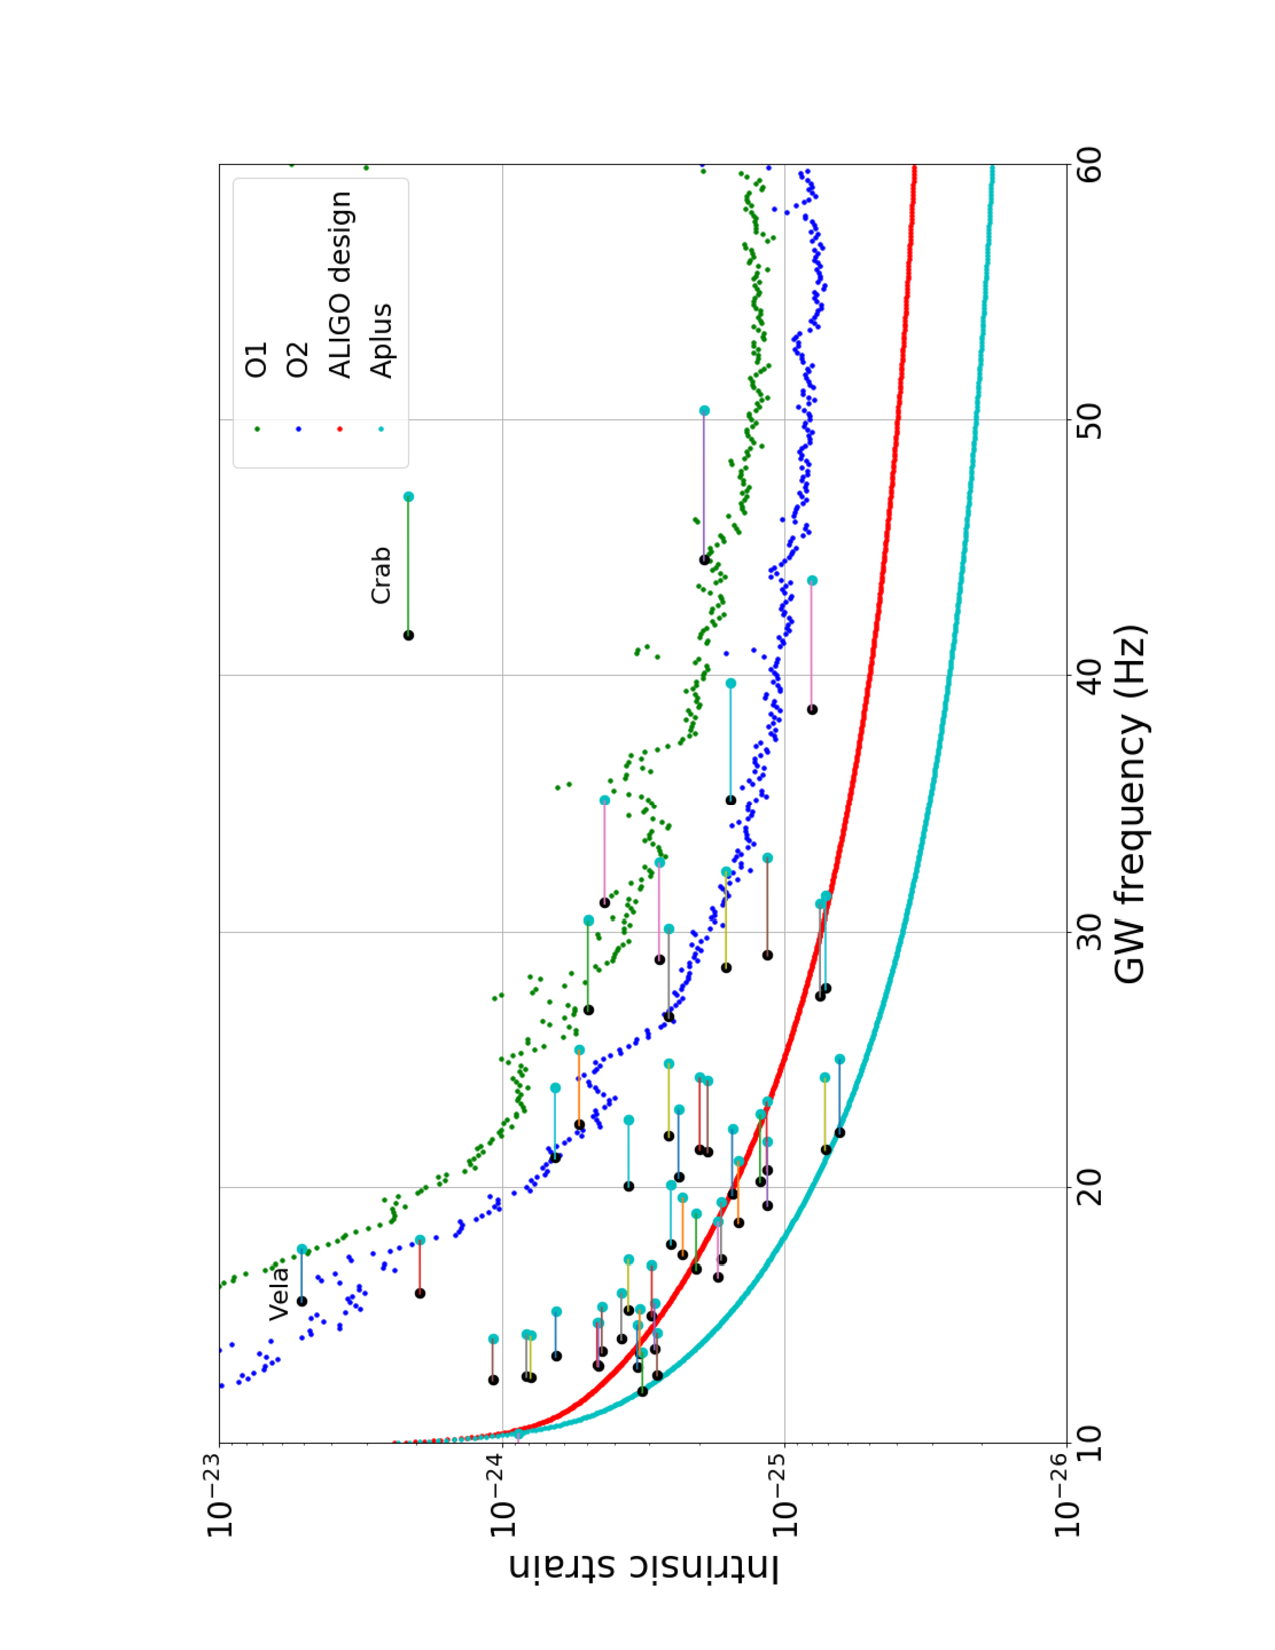
\includegraphics[angle=270,width=\linewidth]{figure/rmeth1}
\caption{
\label{fig1}
Spin-down limits for interesting pulsars (horizontal lines) and sensitivity
estimates (other curves), both in terms of intrinsic strain vs.\ \ac{GW}
frequency.
Spin-down limits are taken from Eq.~(\ref{h0sd}) in the text.
Sensitivity estimates are taken from Eq.~(\ref{h0Td}) and the paragraph
containing it.
}
\end{figure*}

\begin{figure*}
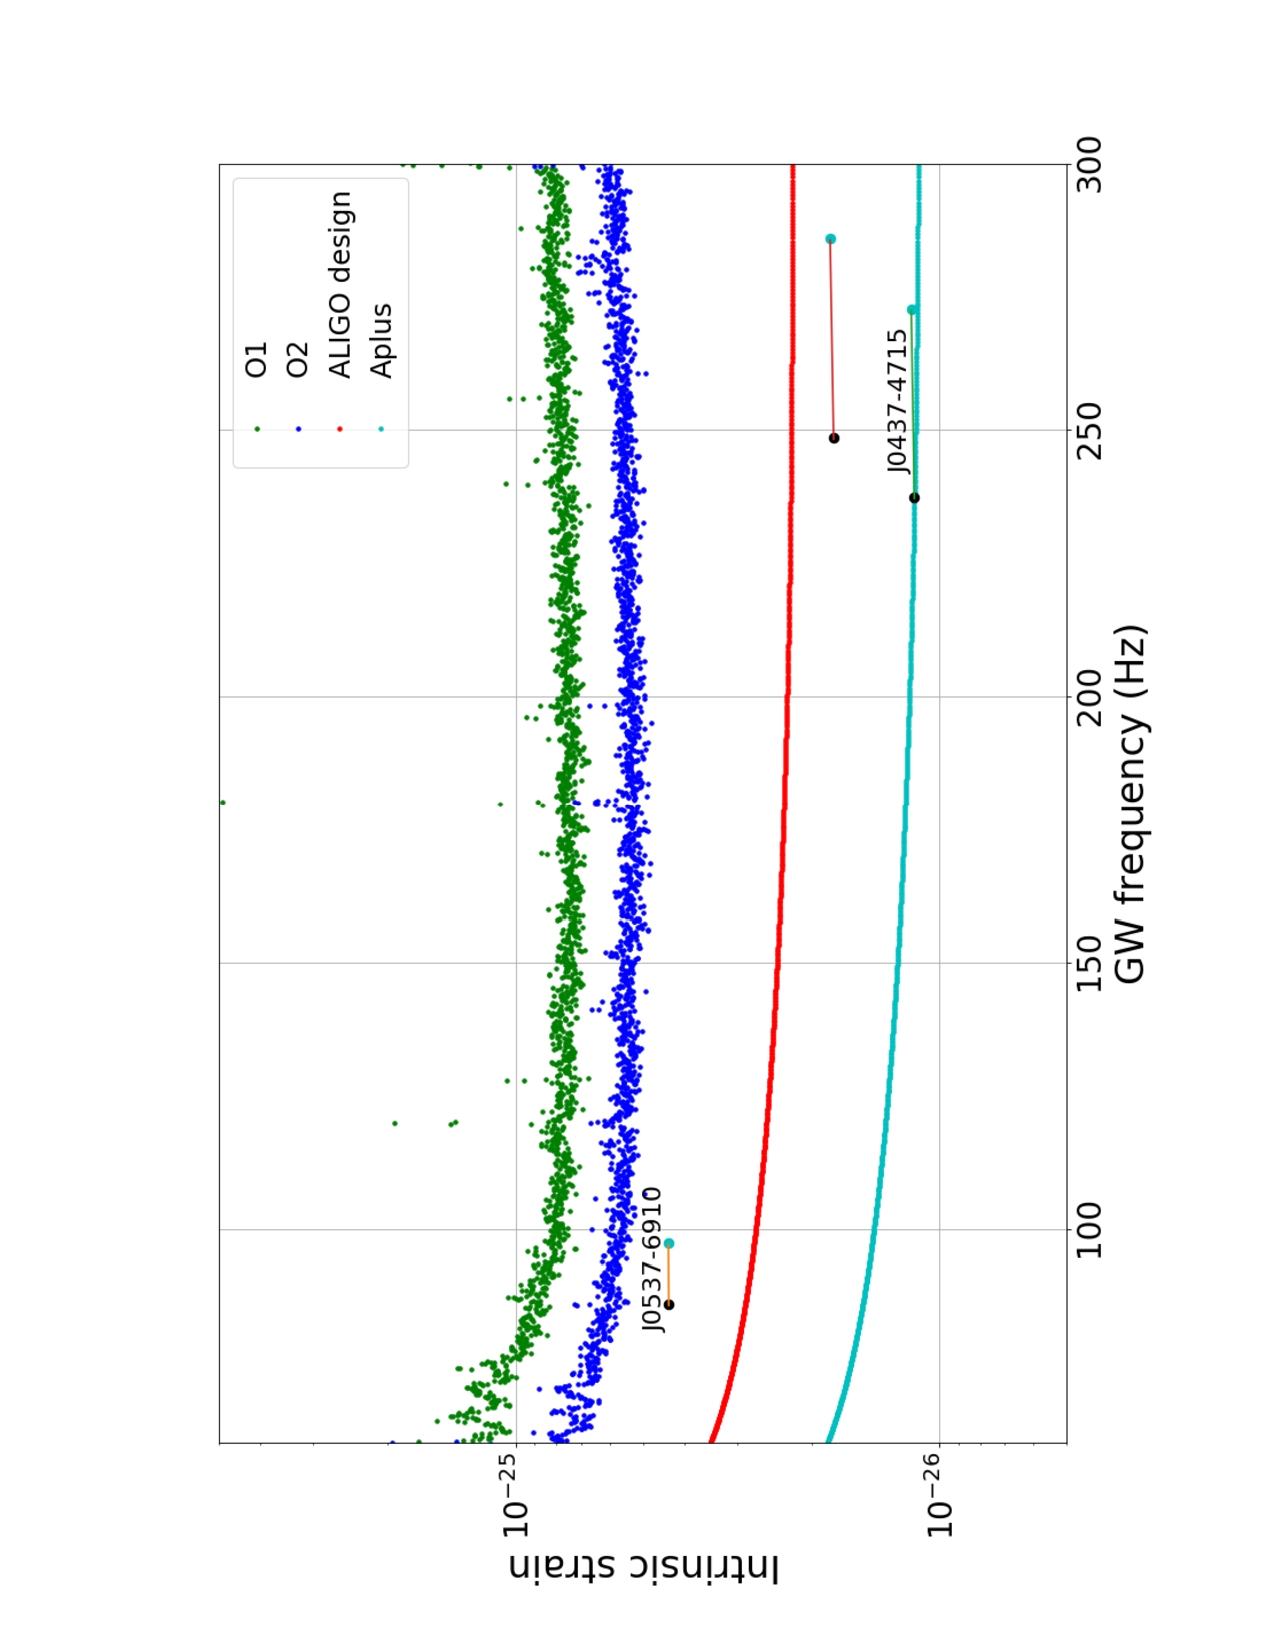
\includegraphics[angle=270,width=\linewidth]{figure/rmeth2}
\caption{
\label{fig2}
Same as the previous figure, for higher frequencies.
There are fewer pulsars here, but the spin-down limits on $r$-mode amplitude
are generally closer to predictions of saturation amplitude.
}
\end{figure*}

We express the sensitivity of each search in terms of upper limits on $h_0$
that can be placed in the absence of a detection.
This is slightly pessimistic---the upper limits are conservative by design and
it is plausible that a somewhat fainter signal could be detected---but it
facilitates comparison with published upper limits from previous searches for
continuous \acp{GW}.
The precise definition of $h_0^\mathrm{UL}$ we use is the same as for instance
in Ref.~\cite{Abbott:2018qee}.
It is a 95\% confidence limit on a population of injected signals with fixed
$h_0$ but varying frequency (within a small band), frequency derivatives, and
angles of inclination and polarization.

The sensitivity of a search of data from a single detector with stationary
noise can be expressed as~\cite{Wette:2011eu}
\begin{equation}
\label{h0Td}
h_0^\mathrm{UL} = \frac{5}{2} \hat\rho \sqrt{ \frac{S_h} {T_d} },
\end{equation}
where $S_h$ is the strain noise \ac{PSD} and $T_d$ is the amount of data.
(In general $T_d$ is less than the integration span $T$ times the number of
interferometers due to maintenance, earthquakes, and so on.)
For multiple detectors or non-stationary noise the \ac{PSD} in
Eq.~(\ref{h0Td}) is replaced by a weighted sum~\cite{Jaranowski:1998qm,
Cutler:2005hc}.
For observations of many days at most sky locations, the sum is very close to
the harmonic mean of noise \acp{PSD}, so we will use the harmonic mean when we
give numbers later.
The statistical factor $\hat\rho$ is iteratively estimated to sufficient
precision using the method of Wette~\cite{Wette:2011eu}, using the template
densities above and assuming that the upper limits are placed on 0.1\,Hz
frequency bands.
(This upper limit band might be chosen differently for different searches, but
its effect on sensitivity is negligible.)
The factor $5\hat\rho/2$ ranges about 33--38 for the searches considered here,
comparable to the factor for directed searches~\cite{Abbott:2018qee} and about
triple the factor for exact timing searches of known
pulsars~\cite{Authors:2019ztc}.
As an alternative, one can write this in terms of sensitivity depth, or the
square root of the \ac{PSD} divided by $h_0$ as in
Ref.~\cite{Dreissigacker:2018afk}.
For the searches considered here, the sensitivity depth is on the order of
110--170\,Hz$^{-1/2}.$
This is comparable to values achieved~\cite{Dreissigacker:2018afk} with narrow
band pulsar searches such as Ref.~\cite{Abbott:2019bed}, or somewhat better
due to longer integration times.
We consider noise \acp{PSD} for \ac{O1}~\cite{H1O1, L1O1}, \ac{O2}~\cite{H1O2,
L1O2}, Advanced LIGO design~\cite{Design}, and the recently funded A+
design~\cite{A+}.
Hence we show four sensitivities:
\ac{O1}, \ac{O2}, and one year integrations at Advanced LIGO and A+ design.

In Figs.~\ref{fig1} and~\ref{fig2} we plot our sensitivity measure vs.\
frequency for the four cases mentioned above, superposed on a set of spin-down
limits for known pulsars from the ATNF catalogue~\cite{Manchester:2004bp}.
Most of the pulsars plotted have already been searched for \acp{GW} at
$f=2\nu$ (and some also at $f=\nu$) in previous LIGO and Virgo papers based on
exact pulsar timing solutions~\cite{Authors:2019ztc}.
Most of the pulsars whose spin-down limits are accessible with existing data
are young and energetic (and sometimes glitchy) like the Crab, and most are
shown in Fig.~\ref{fig1}.
As with known-timing searches, the Crab is the first spin-down limit to become
accessible (already in \ac{O1}), and several more including Vela soon follow.
For later noise curves some middle-aged pulsars (in Fig.~\ref{fig1}) and some
recycled millisecond (in Fig.~\ref{fig2}) pulsars become accessible.
Most notable in Fig.~\ref{fig2} are J0537\textminus6910 and
J0437\textminus4715.
Due to its frequency and proximity to Earth, the latter has
$\alpha_\mathrm{sd}$ of order $10^{-5}$---much lower, and hence more feasible,
than the other accessible pulsars, although $h_0^\mathrm{sd}$ indicates this
pulsar will require at least A+ to detect.

Not all of these pulsars are timed concurrently with LIGO-Virgo observing
runs.
Since the searches proposed here cover broad frequency bands, the uncertainty
in frequency and spin-down parameters is not an issue---unlike the $\nu$ and
$2\nu$ searches.
Our proposed searches do suffer in sensitivity if a pulsar glitches during the
integration, though; and they cannot account for the fluctuating torques
likely in accreting systems.
The glitch issue means that frequent x-ray timing of J0537\textminus6910 will
be important for future \ac{GW} observing runs~\cite{Andersson:2017fow}.

\section{Discussion}

We have shown that searches for continuous \acp{GW} from $r$-modes of known
pulsars can beat the spin-down limits on some pulsars in existing data for
reasonable computational costs.
Although the $r$-mode amplitudes required for detection in such data are
higher than predicted by theory, this work serves as a starting point for
future improvements.
Spin-down limits for many more pulsars will be attainable in the next few
years.

Part of our goal is to point out what theory work could be most important to
help observations.
It is crucial to get the range of mode frequencies and spin-down parameters
right, and helpful to narrow the range down and reduce costs.
Relating frequencies and spin-down parameters more precisely to neutron star
properties will also help measure the latter once a signal is detected.

The most important feature of the search is the $r$-mode frequency range.
Avoided crossings such as that with $t$-modes in the crust could widen the
parameter ranges of some pulsars well beyond what we consider here.
Some pulsars could be undetectable without addressing the avoided crossings
problem.
Updated ranges of the $A$ and $B$ parameters of Eq.~(\ref{fnu}) would also
help in terms of narrowing the parameter space and hence reducing the
computational costs, which will grow to be substantial in coming years.

On the computational side, a pipeline that divides parameter space in a way
suitable for use of the resampled $\mathcal{F}$-statistic~\cite{Patel:2009qe}
would allow for significantly reduced computational cost for long
integrations.

More estimates of saturation amplitudes would be helpful.
This is a very difficult problem, and essentially has been addressed only by
one approach~\cite{Arras:2002dw}.

It would also help to be sure of the coherence time.
If saturated $r$-modes in equilibrium with other modes occasionally experience
phase jumps, this would render long coherent integrations of \ac{GW} data
problematic.

The coherence time issue leads into future work for data analysis:
Accretion and glitches can also introduce issues which encourage development
of alternatives to the straightforward coherent integrations considered here.
Adaptations of semi-coherent techniques developed for other
searches~\cite{Sun:2017zge, Suvorova:2017dpm, Dergachev:2011pd,
Ashton:2018qth} could be fruitful for $r$-modes from known pulsars too.
For those pulsars with a known inclination angle, upgrading from the
$\mathcal{F}$-statistic to the $\mathcal{G}$-statistic will also improve
sensitivity.

\section*{acknowledgments}

We are grateful to the continuous waves search group of the LIGO Scientific
Collaboration, particularly Ian Jones and Karl Wette, for helpful discussions.
This work was supported by NSF grant PHY-1607673.
This paper has been assigned document number LIGO-P1900173.













%%%%%%%%%%%%%%%%%%%%%%%%%%%%%%%%%%%%%%%%%%%%%%%%%%%%%%%%%%%%%%%%%%%%%%%%%%%%%%%%%%%%%%%%%
%%%%%%%%%%%%%%%%%%%%%%%%%%%%%%%%%%%%%%%%%%%%%%%%%%%%%%%%%%%%%%%%%%%%%%%%%%%%%%%%%%%%%%%%%
%%% 							END OF Fourth CHAPTER								  %%%
%%%%%%%%%%%%%%%%%%%%%%%%%%%%%%%%%%%%%%%%%%%%%%%%%%%%%%%%%%%%%%%%%%%%%%%%%%%%%%%%%%%%%%%%%
%%%%%%%%%%%%%%%%%%%%%%%%%%%%%%%%%%%%%%%%%%%%%%%%%%%%%%%%%%%%%%%%%%%%%%%%%%%%%%%%%%%%%%%%%

\chapter{\textbf{Data Analysis}}
\section{Introduction}
Rapidly rotating neutron stars emits continuous gravitational waves due to the
axis asymmetry or oscillation of the fluids. The pulsar are slowly spinning down
due to loss in rotational energy, so the gravitational waves might not
necessarily be monochromatic for a long duration. And, the \acp{GW} are also
Doppler shifted by the daily rotation and orbital motion of the earth. Since,
the interferometer antennae pattern response to the direction of the sources,
the signals are also amplitude modulated due to rotation of earth. The
significant part of the continuous gravitational wave data analysis is to match
the quasi-monochromatic waves to the theoretical waveform. The observational
time needs to be long enough  to extract the \ac{GW} signal buried on
the noisy data. 

The continuous \acp{GW} search can be divided into different categories,
according to the information of the sources. The pulsar like Crab are routinely
monitored in radio observation, so we know the spin frequency and sky
coordinates of Crab pulsar. The neutron star radiates a \ac{GW} twice the spin
frequency due to the mass quadrupole. So, the search with known waveform of the
\ac{GW} is known as Targeted search. They are computationally cheaper and more
sensitive.The $r$-modes frequency deviates from the Newtonian case when
relativistic correction are considered. 
Other type of search is Directed search, the sky coordinates are known but not
the spin frequency. The supernovae remnant like Cassiopeia A are not seen
emitting the pulses, it's probably because the narrow beam of light doesn't
sweep towards the earth. So, a large frequency band is required to search
\ac{GW} from Cassiopeia A which increases the computational cost. The type of
search for unknown neutron star are known as All sky search. There are around
$10^8$ neutron star population in Milky way but only 2000 are observed. Some of
the neutron stars that are not observed in \ac{EM} radiation can be detected in
\ac{GW}.  One of the all sky
search was done for the whole sky from 20 to 1922 Hz~\cite{Abbott_2019a}. Due to
the computational limitation, the all-sky search have short obeservational time
so they are less sensitive than other type of continuous \ac{GW} searches.

\begin{table}[ht]                                                               
\centering                                                                                                                                      
\begin{tabular}{lcccc}                                                          
\hline                                                                          
Type of Search&Sky Location&frequency&Computational Cost&Sensitivity\\          
\hline                                                                          
Targeted&Known&Known&\tikzmark{a}{}&\tikzmark{c}{}\\                            
Narrowband&Known&Known&&\\                                                      
Directed&Known&Unknown&&\\                                                      
All Sky&Unknown&Unknown&\tikzmark{b}{}&\tikzmark{d}{}\\                         
\hline                                                                          
\end{tabular}                                                                   
\link{a}{b}\link{d}{c}                                                          
\caption{Different types of continuous gravitational wave search}
\label{tab}                                                                    
\end{table}         

 On this chapter we will discuss the construction of a signal in
\acp{CW}, the computational cost of the search by looking at the algorithm to
generate template bank. We will also talk about how we claim a detection of real
signals and sensitivity of our search.

\section{Signal Model} 
We here try to iderive the model of the waveform considering both Doppler and
amplitude modutlation of the signal. This will be a summary of the data analysis
paper by \citet{Jaranowski_1998}.

If L is the length of the detector and $\lambda$ the wavelength of gravitational
wave, in long wave approximation $\lambda \gg L$. The time delays of
wave propagating over the detector are negligible ($\Delta \approx $), so
gravitational wave field can be treated as being uniform all over the detector.
Let h be the relative change of arm length of detector when gravitational waves
passes by.
\begin{equation}
h(t) = \frac{1}{2} n_1.[\tilde{H}(t)n_1] - \frac{1}{2} n_2. [\tilde{H}(t)n_2]
\end{equation}
where $n_1=(1,0,0)$ and $n_2=(0,1,0)$ denotes a unit vectors parallel to the
detector arm, assuming $n_1 \perp n_2$. And $\tilde{H}$ is defined as:
\begin{equation}
\tilde{H}(t) = M(t)H(t)M(t)^T,
\end{equation}
\begin{equation*}
H(t)=
\begin{pmatrix}
h_+(t) & h_\times(t) 0\\
h_\times(t) & -h_+(t) & 0\\
0 & 0 & 0
\end{pmatrix}
\end{equation*}
where, $h_+$ and $h_\times$ are plus and cross polarization of \acp{GW}.
\begin{equation}
M= M_3 M_2 M_1
\end{equation}
where,
$M_1 \rightarrow \text{transformation matrix from wave to celestial sphere with
Euler angle($\alpha,\delta,\Psi$)}$\\
$M_2 \rightarrow \text{celestial coordinates to cardinal coordinates with Euler
angle}$\\
$M_3 \rightarrow \text{from cardinal to detector reference frame}$

\begin{equation}
M_1=
\begin{pmatrix}
\cos{-\Psi} & \sin{-\Psi}& 0\\
-\sin{-\Psi} & \cos{\Psi}& 0\\
0 & 0 & 1
\end{pmatrix}
\begin{pmatrix}
1 & 0 & 0\\
0 & \cos{(-\frac{\pi}{2}-\delta)} & \sin{(-\frac{\pi}{2}-\delta)}\\
0 & -\sin{(-\frac{\pi}{2}-\delta)} & cos{(-\frac{\pi}{2}-\delta)}
\end{pmatrix}
\begin{pmatrix}
\cos{(\frac{\pi}{2}-\alpha)} & \sin{(\frac{\pi}{2}-\alpha)} & 0\\
-\sin{(\frac{\pi}{2}-\alpha)} & \cos{(\frac{\pi}{2}-\alpha)} & 0\\
0 & 0 & 1 
\end{pmatrix}
\end{equation}
\begin{equation}
M_2=
\begin{pmatrix}
\sin{\lambda}\cos{(\phi_r+\Omega_rt)} & \sin{\lambda}\sin{(\phi_r+\Omega_rt)} 
& -cos{\lambda}\\
-sin{()\phi_r+\Omega_rt)} & \cos{(\phi_r+\Omega_rt)} & 0\\
\cos{\lambda}\cos{(\phi_r+\Omega_rt)}  & \cos{\lambda}\sin{(\phi_r+\Omega_rt)} 
& sin{\lambda}
\end{pmatrix}
\end{equation}

\begin{equation}
M_3=
\begin{pmatrix}
\cos{(\frac{\pi}{2}+\gamma)} & \sin{(\frac{\pi}{2}+\gamma)} & 0\\
-\sin{(\frac{\pi}{2}+\gamma)} & \cos{(\frac{\pi}{2}+\gamma)} & 0\\
0 & 0 & 1
\end{pmatrix}
\end{equation}

\begin{figure}[h!]
  \centering
  \begin{minipage}{0.4\textwidth}
    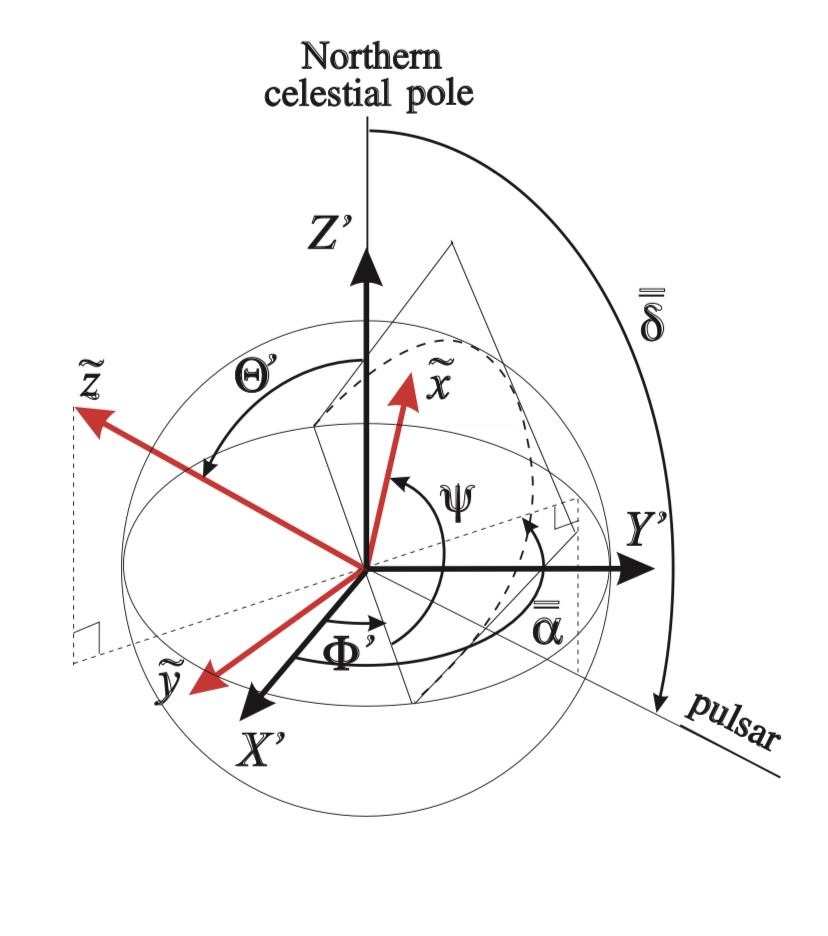
\includegraphics[width=\textwidth]{figure/wavedetector.jpg}
  \end{minipage}
  \hfill
  \begin{minipage}{0.6\textwidth}
    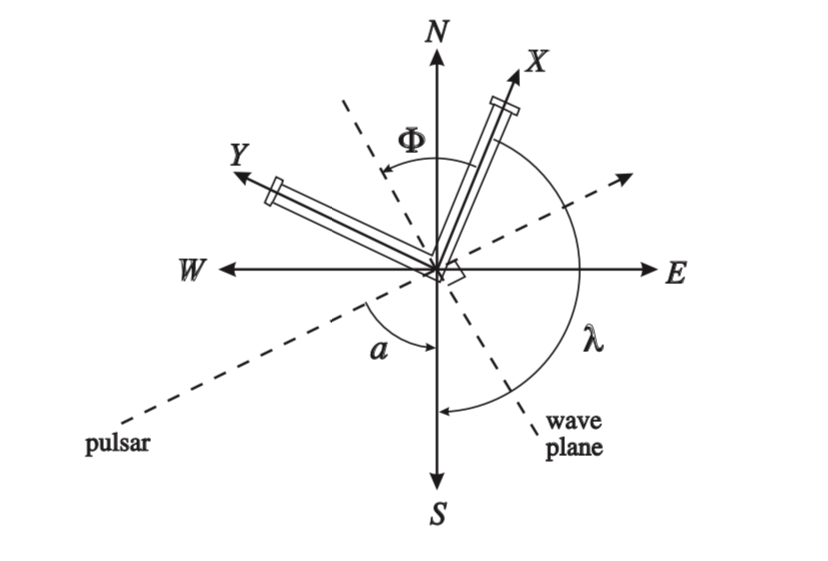
\includegraphics[width=\textwidth]{figure/wavecelestial.jpg}
  \end{minipage}
  \caption{Coordinate transformation from wave frame to detector frame. Image
   from~\cite{1996A&A...312..675B}}
  \label{fig:Wavetodetector}
\end{figure}

The response of the interferometer is given by:
\begin{equation}
h(t) = F_+(t) h_+(t) + F_\times(t) h_\times(t) 
\end{equation}

And $F_+$ and $F_\times$ are the antennae pattern. The antennae pattern are periodic
functions of time, and its period is one day. The antennae pattern are the
functions of right ascension($\alpha$), declination($\delta$) of the \acp{GW}
sources and polarization angle($\Psi$). 

The antennae pattern $F_+$ and $F_\times$ can be written as:
\begin{align*}
F_+(t) = a(t)cos(2\Psi) + b(t) sin(2\Psi)\\
F_\times(t) = b(t)cos(2\Psi) - a(t) sin(2\Psi)
\end{align*}
where,
\begin{align*}\label{a}
a(t) &=
\frac{1}{16}\sin{2\gamma}(3-\cos{2\lambda})(3-\cos{2\delta})\cos{[2(\alpha-\phi_r-\Omega_rt)]}\\
&-\frac{1}{4}\cos{2\gamma} \sin{\lambda} (3-\cos{2\delta})
\sin{[2(\alpha-\phi_r-\Omega_rt)]}
+\frac{1}{4}\sin{2\gamma} \sin{2\lambda} \sin{2\delta}
\cos{[\alpha-\phi_r-\Omega_r t]} \\
&-\frac{1}{2}\cos{2\gamma} \cos{\lambda} \sin{2\delta}
\sin{[\alpha-\phi_r-\Omega_r t]}
+\frac{3}{4} \sin{2\gamma} \cos^2{\lambda} \cos^2{\delta}
\end{align*}
\begin{align*}
b(t)& =\cos{2\gamma} sin{\lambda} \sin{\delta} \cos{[2(\alpha-\phi_r-\Omega_r
t)]} +
\frac{1}{4} \sin{2\gamma} (3-\cos{2\lambda}) \sin{\delta}
\sin{[\alpha-\phi_r-\Omega_rt]}\\
&+ \cos{2\gamma} \cos{\lambda} \cos{\delta} \cos{[\alpha-\phi_r-\Omega_r t]} +
\frac{1}{2}\sin{2\gamma} \sin{2\lambda} \cos{\delta}
\sin{[\alpha-\phi_r-\Omega_rt]}
\end{align*}
where,\\
$\lambda \rightarrow \text{latitude of detector}$\\
$\Omega_r \rightarrow \text{rotational angular velocity of earth}$\\
$\phi_r \rightarrow \text{phase which defines the position of the Earth in its
diurnal motion}$\\
$\phi_r + \Omega_r t \rightarrow$ local sidereal time of the detector[the
angle between local meridian and the vernal point].\\
$\gamma \rightarrow \text{orientation of the detector's arms with respect to
geographical direction.}$\\
This is the transformation using the rotation matrix from wave frame to the
detector frame. 

The gravitational waves signal can be written in terms of Doppler
parameter($\alpha, \delta, f, f_n $) and amplitude parameter($h_0, \iota, \psi,
\phi$):
\begin{equation}
h(t) = \sum_{i=1}^{4}A_{1i} h{1i}(t) + \sum_{i=1}^{4} A_{2i} h{2i}(t)
\end{equation}
The amplitudes $A_{1i}$ and $A_{2i}$ are given by:
\begin{align*}
A_{11} = h_0 \sin{2\theta}\left[\frac{1}{8} \sin{2\iota}\cos{2\psi}\cos{\phi_0}-
\frac{1}{4}\sin{\iota} \sin{2\psi}\sin{\psi_0}\right], \\
A_{12} = h_0 \sin{2\theta}\left[\frac{1}{4} \sin{iota}\cos{2\psi}\sin{\phi_0}+
\frac{1}{4}\sin{2\iota} \sin{2\psi}\cos{\psi_0}\right], \\
A_{13} = h_0 \sin{2\theta}\left[-\frac{1}{8} \sin{2\iota}\cos{2\psi}\sin{\phi_0}
-\frac{1}{4}\sin{\iota} \sin{2\psi}\cos{\psi_0}\right], \\
A_{14} = h_0 \sin{2\theta}\left[\frac{1}{4} \sin{2\iota}\cos{2\psi}\cos{\phi_0}-
\frac{1}{8}\sin{2\iota} \sin{2\psi}\sin{\psi_0}\right], \\
A_{21} = h_0 \sin^2{\theta}\left[\frac{1}{2}
(1+\cos^2{\iota})\cos{2\psi}\cos{2\phi_0}- \cos{\iota} \sin{2\psi}\sin{2\psi_0}\right], \\
A_{22} = h_0 \sin^2{\theta}\left[\frac{1}{2}
(1+\cos^2{\iota})\sin{2\psi}\cos{2\phi_0} + \cos{\iota} \cos{2\psi}\sin{2\psi_0}\right], \\
A_{23} = h_0 \sin^2{\theta}\left[-\frac{1}{2}
(1+\cos^2{\iota})\cos{2\psi}\sin{2\phi_0}- \cos{\iota} \sin{2\psi}\cos{2\psi_0}\right], \\
A_{24} = h_0 \sin^2{\theta}\left[-\frac{1}{2}
(1+\cos^2{\iota})\sin{2\psi}\sin{2\phi_0} + \cos{\iota} \cos{2\psi}\cos{2\psi_0}\right], \\
\end{align*}
And the dependent Doppler functions $h_{i}$ are:
\begin{equation}\label{h}
h_{1}=a(t) \cos{\phi(t)},\quad h_{2}=b(t) \cos{\phi(t)}\\ 
h_{l3}=a(t) \sin{\phi(t)},\quad h_{4}=b(t) \sin{\phi(t)} 
\end{equation}
where, a(t) and b(t) are defined in \ref{a}.



\subsection{Maximum Likelihood ratio}

The data from the gravitational waves interferometer are subject to various
noise sources and the signals($h(t)$) are buried under the noises($n(t)$). The challenging part
of \ac{GW} astronomy are to extract the weak signals from the random noises,
most of the computational power are needed to filter out the noises. The
detector data $x(t)$ can be written as :
\begin{equation}
x(t) = h(t)+n(t)
\end{equation}
The maximum likelihood ratio can be defined as ratio of the probability density function
of when signal is present to when signal is absent.
\begin{equation}\label{eqn:lhood}
\Lambda = \frac{p(x|h+n)}{p(x|n)}
\end{equation}
Assuming the noise is a zero mean, stationary, Gaussian random process and
variance unity, the probability density function of noise will be:
\begin{align*}
p(x|n) & = \mathcal{N}exp(-(x-0)^2/(2*1))\\
&= \mathcal{N}exp(-\frac{1}{2}(x|x))
\end{align*}
Similarly, if the data contains a signal h, now the mean will be h.
\begin{equation}
p(x|h+n)= \mathcal{N}exp(-\frac{1}{2}(x-h|x-h))
\end{equation}
Now, the likelihood ratio~\ref{eqn:lhood} can be written as:
\begin{equation}
\Lambda= \frac{exp(-\frac{1}{2}(x|x)}{exp(-\frac{1}{2}(x-h|x-h))}
\end{equation}
Taking, the log of likelihood ratio:
\begin{align*}
\ln{\Lambda} & =-\frac{1}{2}(x-h|x-h) + \frac{1}{2}(x|x)\\
& = \cancel{-\frac{1}{2}(x|x)} +(x|h)-\frac{1}{2}(h|h)+\cancel{\frac{1}{2}(x|x)}
\end{align*}
The log likelihood function can be written as:
\begin{equation}
\ln{\Lambda}=(x|h)-\frac{1}{2}(h|h)
\end{equation}
where the scalar product is defined as:
\begin{equation}
(x|y)=4\mathcal{R} \int_{0}^{\infty}\frac{\tilde{x}(f)\tilde{y}^*(f)}{S_h(f)}df, 
\end{equation}
where, $\tilde{x}$ is the Fourier transform, $^*$ is the complex conjugate and 
$S_h$ is the power spectral density of the detector noise.

The signal $h(t,\vec{A},\vec{\lambda})$ depends linearly on the amplitudes parameter(A)
$h_0$, $\theta$, $\psi$, $\iota$ and $\phi$. The maximum value of the likelihood
function can be found by:
\begin{equation}
\frac{\partial\ln\Lambda}{\partial A_i}= 0, \quad i=1,....,4.  
\end{equation}

\begin{equation}
\sum_{j=1}^4M_{ij}A_j =(x||h_i),
\end{equation}
where M is a $4 \times 4$ matrix given by:
\begin{equation}
M_{ij} = (h_i|h_j)
\end{equation}
where,
\begin{equation}
(h_i||h_j)=\frac{2}{T_0}\int_{-T_0/2}^{T_0/2}h_i(t)h_j(t)dt, \quad
T_0 \rightarrow \text{observational time.}
\end{equation}
From Eqn.\ref{h} $h_1$ $\&$ $h_2$ $\propto$ $\cos{\phi(t)}$\quad and $h_3$ $\&$ $h_4$
$\propto$ $\sin{\phi(t)}$, so,
\begin{equation}
(h_1||h_3)=0, \quad (h_1||h_4)=0, \quad (h_2||h_3)=0, \quad (h_2||h_4)=0,  
\end{equation}
and
\begin{equation}
\begin{split}
(h_1||h_1)=(h_3||h_3)=\frac{1}{2}A,\\
(h_2||h_2)=(h_4||h_4)=\frac{1}{2}B,\\
(h_1||h_2)=(h_3||h_4)=\frac{1}{2}C,\\
\end{split}
\end{equation}
where, $A=(a(t)||a(t))$, \quad  $B=(b(t)||b(t))$, \quad  $C=(a(t)||b(t))$ 
\begin{equation*}
M=\frac{1}{2}
\begin{pmatrix}
A & C & 0 & 0\\
C & B & 0 & 0\\
0 & 0 & A & C\\
0 & 0 & C & B
\end{pmatrix}
\end{equation*}
The $\mathcal{F}$-statistic is the maximization of likelihood function over
$\vec{A}$. 
\begin{equation}
2\mathcal{F}(\vec(\lambda))=\sum_{i,j=1}^{4}[M^{-1}]_{ij}(x||h_i)(x||h_j)
\end{equation}
where,
\begin{equation*}                                                               
M^{-1}=\frac{2}{D}                                                                   
\begin{pmatrix}                                                                 
B & -C & 0 & 0\\                                                                 
-C & A & 0 & 0\\                                                                 
0 & 0 & B & -C\\                                                                 
0 & 0 & -C & A                                                                   
\end{pmatrix}                                                                   
\end{equation*} 
where, $D=AB-C^2$
\begin{equation}
2\mathcal{F}=\frac{2}{D}\left[B(x||h_1)^2 + A(x||h_2)^2 -2C(x||h_1)(x||h_2)+
B(x||h_3)^2 + A(x||h_4)^2 -2C(x||h_3)(x||h_4)\right]
\end{equation}
Since the 2$\mathcal{F}$ is maximized over the amplitude parameter, so it is the
function of remaining Doppler parameter($\vec{\lambda}\rightarrow \alpha,\delta,f^n$). The signal
template $h(t,\vec{A},\vec{\lambda})$ is not linear function of Doppler
parameter($\vec{\lambda}$), we need to find maximum 2$\mathcal{F}$ value over
$\vec{\lambda}$ analytically. 

First, we need to calculate the probability density of $2\mathcal{F}$ when
signal is present and when signal is absent. The detection of signal is claimed
when the $2\mathcal{F}$ beats the certain threshold level with given False Alarm
rate. 

Lets suppose we know $h_i$ i.e. the sky position and spin down parameters. When
the signals are absent $(x||h_i)$ = 0. To make the calculation easier, lets
assume the observational time is the integer multiple of one sidereal day, so $C
= 0$~\cite{Jaranowski_2000}. When the signal is present:
\begin{equation}
(x||h_1)= \frac{1}{2}AA_1, \quad (x||h_2) = \frac{1}{2}B A_2\\
(x||h_3)= \frac{1}{2}AA_3, \quad (x||h_4) = \frac{1}{2}B A_4
\end{equation}
Now, we can define $\mathcal{F}$-statistic as:
\begin{equation}
\mathcal{F} = \frac{1}{2}(z_1^2+z_2^2+z_3^2+z_4^2)
\end{equation}
where,
\begin{equation}
z_1=2\sqrt{\frac{T_0}{S_hA}}(x||h_i), \quad i=1,3
\end{equation}
\begin{equation}
z_1=2\sqrt{\frac{T_0}{S_hB}}(x||h_i), \quad i=2,4
\end{equation}
In absence of signal the $2\mathcal{F}$ is chi-squared distribution with four
degrees of freedom. And, when the signals are present, the $2\mathcal{F}$ is a
non-central chi-squared distribution with four degrees of freedom and non
centrality parameter is the optimal signal to noise ratio(d) defined as:
\begin{equation}
d^2=\frac{2}{S_h(f)}\int_0^{T_0} h^2(t)dt
\end{equation}

The probability density functions when signal is absent($p_0$)and when signal is
present($p_1$) is:
\begin{equation}
\begin{split}
p_0(\mathcal{F})&=\frac{\mathcal{F}^3}{6}exp{-\mathcal{F}},\\
p_1(d,\mathcal{F})&=\frac{2\mathcal{F}^3/2}{d^3}I_3(d\sqrt{2\mathcal{F}})exp{-\mathcal{F}-\frac{1}{2}d^2},
\end{split}
\end{equation}
where $I_3$ is the modified Bessel function of first kind and order 3.
The expectation value of 2$\mathcal{F}$ is 4+$d^2$.
\begin{figure}[h!]
	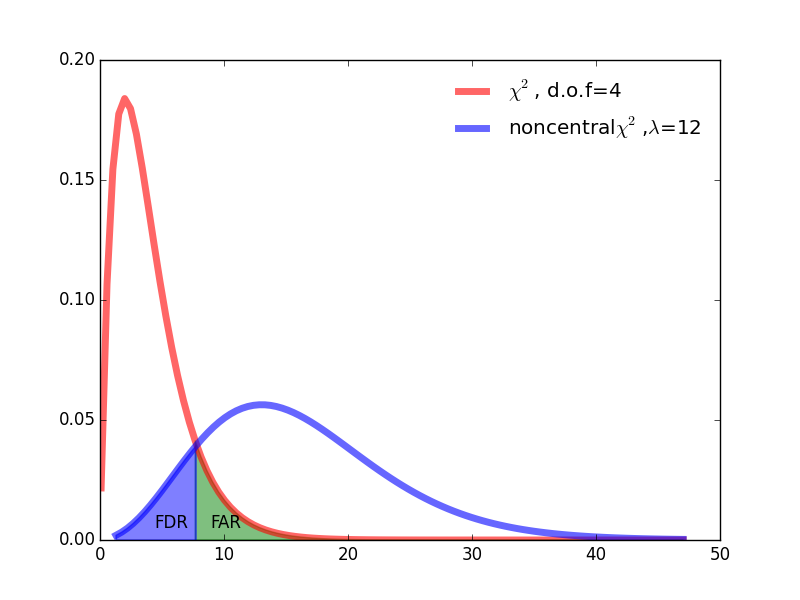
\includegraphics[width=\textwidth]{figure/chi2.png}
	\caption{In absence of signal the pdf will be $\chi^2$ distribution with
four degrees of freedom. In presence of signal the pdf will be non central
$\chi^2$ distribution where the non central parameter is the signal.}
\end{figure}

\subsection{Matched Filtering technique}
Matched filter is a optimal technique of maximizing the signal to noise ratio by
cotrrelating the detector data with a known waveform~\cite{Sathyaprakash_2009}.
The detector output x(t) contains a signal h(t) and noise n(t), and let q(t) be
a template of known shape. Let c be the correlation between the template and
detector output:
\begin{equation}\label{eq:matchfil1}
c(\tau) = \int_{-\infty}^{\infty} x(t)q(t+\tau)dt
\end{equation}
where $\tau$ is the time delay between the template and the detector data.
The time series data can be converted into frequency domain using the Fourier
transform. 
\begin{equation}\label{eq:matchfil2}
\begin{split}
x(t)=\int_{-\infty}^{\infty} x(f)e^{2\pi f t} df
q(t+\tau)\\
&=\int_{-\infty}^{\infty} q(f)e^{2\pi\tilde{f}(t+\tau)} d\tilde{f}
\end{split}
\end{equation}
Substituting equation ~\ref{eq:matchfil2} into \ref{eq:matchfil1},

\begin{align*}
c(\tau) &= \int_{-\infty}^{\infty} dt \int_{-\infty}^{\infty}
df\int_{-\infty}^{\infty} df^{'} \tilde{x}(f)\tilde{q}^*(f^{'}) e^{-i2\pi
ft}e^{i2\pi f^{'}(t+\tau)}\\
  & = \int_{-\infty}^{\infty} df \int_{-\infty}^{\infty} df^{'}
\tilde{x}(f)\tilde{q}^*(f^{'})\underbrace{\int_{-\infty}^{\infty} dt e^{-i 2\pi
(f-f^{'})t}}_{\delta(f-f^{'})}
e^{i 2\pi f^{'}\tau}\\
 & = \int_{-\infty}^{\infty}\tilde{x}(f)\tilde{q}(f)e^{i 2\pi f^{'}\tau}
\int_{-\infty}^{\infty} df^{'}\delta(f-f^{'})\\
 & = \int_{-\infty}^{\infty}\tilde{x}(f)\tilde{q}(f)e^{i 2\pi f^{'}\tau}
\end{align*}
The \ac{SNR} is defined as $\frac{\mu}{\sigma}$, where $\mu=<c>$ is a mean and
$\sigma$ is a standard deviation of the correlation.

\begin{align*}\label{eq:sign}
\mu & = <\int_{-\infty}^{\infty}\tilde{q}^{*}(f)\tilde{x}(f)>\\
&=\int_{-\infty}^{\infty}\tilde{q}^{*}(f)\tilde{h}(f)
\end{align*}

\begin{equation}\label{eq:noise1}
\begin{split}
\sigma^{2} & =<\int_{-\infty}^{\infty}\tilde{q}(f)\tilde{n}^{*}(f)df
\int_{-\infty}^{\infty} \tilde{q}^{*}(f^{'}) \tilde{n}(f^{'})df^{'}>\\
       &= \int_{-\infty}^{\infty}df|\tilde{q}(f)|^{2}
\int_{-\infty}^{\infty}\underbrace{\tilde{n}^{*}(f)
\tilde{n}(f^{'})}_{S_{n}(f)\delta(f - f^{'})}df^{'}\\
      &=\int_{-\infty}^{\infty}df|\tilde{q}(f)|^{2} S_{n}(f)
\end{split}
\end{equation}
From \ref{eq:sign} and \ref{eq:noise1}, we can get \ac{SNR}.
\begin{equation}
\rho=\frac{\int_{-\infty}^{\infty}\tilde{q}^{*}(f)\tilde{h}(f)}{(\int_{-\infty}^{\infty}df|\tilde{q}(f)|^2
S_{h}(f))^{1/2}}
\end{equation}
The optimal signal to noise ratio is defined as:
\begin{equation}
\rho_{opt}^2 = <h,h> =2\left[\int_{0}^{\infty}\frac{|\tilde{h}(f)|^2}{S_{h}}(f){}df\right]
\end{equation}
So, the optimal \ac{SNR} is the total energy of the signal weighted down by the
\ac{PSD} of noise. So, if the \ac{PSD} of noise at some frequency bin is higher,
the \ac{SNR} will be lower.


\subsection{Phases of gravitational waves}
The pulsars are spinning down by the emission of particles, \ac{EM} and \ac{GW}.
The frequency evolution are given by the Taylor expansion in the form:
\begin{equation}
f(t) = f_0 + \sum_{n=1}^{N} \frac{f_n}{n!}t^n
\end{equation}
where, $f_n$ are the spin down parameter. Usually, for less than one year of
search we don't need more than two spin down parameter. 
The frequency($f_0$) of gravitational waves from the source are Doppler modulated due to the
rotation of earth, so the apparent frequency($f_\prime$) is given by:
\begin{equation} 
f^\prime = f_0 \left(1+\frac{\vec{v}.\hat{r}}{c}\right)
\end{equation}
where, v is the relative velocity of source with respect to detector, $\hat{r}$
is the unit vector from the detector to the sources and c is the speed of light.

So, the frequency of gravitational waves($f_{gw}$) in Solar System Barycenter
(SSB) frame is~\cite{Krishnan_2004}:
\begin{equation}
f_{gw}(t) = f_0 + \sum_{n=1}^{N} \frac{f_n}{n!}\left(t - t_0 + \frac{\Delta
\vec{r}(t). \vec{n}}{c}\right)^n
\end{equation}
where, $t_0$ is a detector time in the start of observation, and we are
neglecting the proper motion of neutron stars. 

\section{Short time baseline Fourier Transforms}
The pulsars are slowly spinning down, and the frequency of gravitational waves
in the interferometer will be Doppler modulated due to the rotation of earth.
As, the frequency of \ac{GW} modulated, the match filtering the one chunk of
data for the whole observational time will be inconvenient. And, the
interferometer noises are also non stationary, so the interferometer data are 
divided into N segments and Fourier transformed. The computational cost of the
search increases linearly with the number of \acp{SFT} for a fixed observational
time. There are two main points accounted for making \acp{SFT},(i) the time of the
\acp{SFT} should be short enough for the detector noises to remain constant, (ii)
long enough for the signal power to stay within the frequency bin, as the
frequency change due to Doppler modulation and spin
down~\cite{Krishnan_2004,Abbott_2007}. 

We are deriving the maximum \ac{SFT} time such that the signal stays within half
of the frequency bin as shown in \citet{Krishnan_2004}. The frequency at the detector can be given by the Doppler formula:
\begin{equation}
\label{doppler}
f_d(t) - f_s(t) = f_s(t)\frac{\vec{v}(t).\hat{n}}{c}
\end{equation}
where, $f_s$ is the frequency at the Solar System Barycenter(SSB) frame and
$\vec{v}$ is the velocity of the detector.
The rate of frequency change due to Doppler effect can calculated by taking
derivative of Eqn \ref{doppler}.
\begin{equation}
\dot{f}_= \frac{f_s}{c}\frac{d\vec{v}}{dt}.\hat{n} \leq
\frac{f_s}{c}\left|\frac{d\vec{v}}{dt}\right|
\end{equation}
The term $dv/dt=acceleration$, and it can be written as $a=v^2/R$, where R is
the radius of earth. And we can also substitute $v=2\pi R/T$ where, T is the time
period of rotation of earth.
\begin{equation}\label{sfts1}
|\dot{f}|_{max}= \frac{4\pi^2R}{T}
\end{equation}
For the signal, to stay within the half of the frequency bin, it need to satisfy
the condition $|\dot{f}|T_{SFTs} < \frac{1}/{2T_{SFTs}}$, or it can be written as:
\begin{equation}\label{sfts2}
T_{SFTs}<\sqrt{\frac{1}{2|\dot{f}_{max}|}}
\end{equation}
Substituting \ref{sfts1} in \ref{sfts2}, we get,
\begin{equation}
T_{SFTs} < 18.5 \text{hours}\sqrt{\frac{1}{f_s}}
\end{equation}
So, for a pulsar emitting a \ac{GW} of frequency 100 Hz, the time of the
\ac{SFT} should be less than 1.85 hours. For our search, we are using \acp{SFT} of 30 minutes.


\section{Template Spacing}
In a matched filtering technique the shape of the signal that will the detected
by gravitational wave interferometer needs to be well known. The shape are
determined by the sky location, frequency and the frequency derivatives of the
sources. The intrinsic strain, polarization amplitude, inclination angle, and
initial phase of a signal are not known so these parameter are maximized. In a
directed search, the shape of the known is not well know due to the lack of
information on spin frequency of the sources. And in $r$-modes \ac{GW} search
from known pulsar, the spin frequency are known but we don't know the exact
$r$-mode frequency due to the unknown compactness of neutron stars. When the
exact waveform is not known, we need a multiple templates that possibly can
match with a signal. The template spacing should consider both computational
cost and the loss in signal to noise ratio. If the distance between templates are two far away
and the signal lies in between templates we will loose the significant amount of
\ac{SNR}. And, if the templates are too dense we will wasting a computational
power.  Lets match the signal $h(t,\vec{A},\vec{\lambda})$ with a little offset template
 $h(t,\vec{A},\vec{\lambda}+\Delta\vec{\lambda})$, the match is defined
as~\cite{Owen_1996}:
\begin{equation}
M(\vec{\lambda}+\Delta\vec{\lambda}) =
max<h(t,\vec{A},\vec{\lambda})|h(t,\vec{A},\vec{\lambda}+\Delta\vec{\lambda})>
\end{equation}
This can be expanded in power series about $\Delta\lambda=0$:
\begin{equation}\label{match}
M(\lambda,\Delta\lambda)\approx
1+\frac{1}{2}\left(\frac{\partial^2M}{\partial\Delta\lambda_i\partial\Delta\lambda_j}\right)_{\Delta\lambda^k=0}
\Delta\lambda^i\Delta\lambda^j
\end{equation}
We can define a metric 
\begin{equation}
g_{ij}(\lambda)=-\frac{1}{2}\left(\frac{\partial^2M}{\partial\Delta\lambda_i\partial\Delta\lambda_j}\right)_{\Delta\lambda^k=0}
\end{equation}
Now, Eqn~\ref{match} can be written as:
\begin{equation}
1-M=g_{ij} \Delta\lambda^i\Delta\lambda^j
\end{equation}
where 1-M is the mismatch between two templates.

We define a parameter minimal match($\mu$) as the maximum loss in signal to
noise ratio when the signal lies exactly in between two nearest templates. 
We can also define $\mu$ as a mismatch between the signal with Doppler
parameter($\vec{\lambda}$) with
expectation value $2\mathcal{F}(\vec{\lambda})$ with a template
$2\mathcal{F}(\vec{\lambda}')$. 
\begin{equation}
\mu(\vec{\lambda},\vec{\lambda}')=\frac{2\mathcal{F}(\vec{\lambda})-2\mathcal{F}(\vec{\lambda}')}{2\mathcal{F}(\vec{\lambda})}
\end{equation}

The template density for a search with known spin frequency(f) and spin
down($\dot{f},\ddot{f}$)
parameter of pulsar is given by:
\begin{equation}
N=\frac{\sqrt{det|g_{ij}|}}{2(1-\mu)}\int d\dot{f}\ddot{f}
\end{equation}
where, the metric($g_{ij}$) over the parameters f, $d\dot{f}$, $\ddot{f}$ is given
by~\cite{Wette_2008}:
\begin{equation}                                                                
g_{ij}=\frac{4\pi^2T^{i+j+2}(i+1)(j+1)}{(i+2)!(j+2)!(i+j+3)}             
\end{equation}\\                                                                
                                                                                
\text{i,j=0 for $f$, 1 for $\dot{f}$ and 2 for $\ddot{f}$}; $T           
=\text{Time of observation}$                                                              
\begin{equation} 
g_{ij} = \pi^2                                                 
\begin{pmatrix}
T^2/3 & T^3/6 & T^4/20 \\                                                       
T^3/6 & 4T^4/45 & T^5/36 \\                                                     
T^4/20 & T^5/36 & T^6/112                                                       
\end{pmatrix}
\end{equation} 

So, the number of templates depends on the duration of the search, and the
number of spin down parameters. The computational cost for a directed search
with known sky location but unknown $f,\dot{f},\ddot{f}$ will be $f*T^7$. But,
the sensitivity of the search only increases by $\sqrt{T}$.

\section{Hypothesis testing}                                                    
        When we analyze a data and claim a detection we need to perform certain
test on a sample of data. If our experiment results are from purely chance then
it is defined as Null hypothesis($H_o$) and if the results rejects the null
hypothesis we define as alternative hypothesis. The alternative hypothesis are
usually the one researcher looking for.  In our search if signal is absent it is
called null hypothesis and if signals are present we call it alternative
hypothesis.
	In statistical test there are two kind of error in the experimental
results. The type I error(False alarm probability) is when the experimenter
chooses $H_a$ when $H_o$ is true.  The type II error (False Dismissal
Probability) is when the researcher chooses $H_o$ when $H_a$ is true.  So, in
Type I error the test value is greater than the threshold significance level
when no signal are present. And, in type II error the test value is less than
the threshold when there are actually signal in the data.
As shown in figure the probability of False Alarm Rate is defined as:
\begin{equation}
P_{FAR}=P(2\mathcal{F}>2\mathcal{F}^*|H_o)=\int_{2\mathcal{F}^*}^\infty
pdf(2\mathcal{F}|H_o)d2\mathcal{F}
\end{equation}
And, the equation of False Dismissal Rate is given by:
\begin{equation}
P_{FDR}=P(2\mathcal{F}<2\mathcal{F}^*|H_a)=\int_{-\infty}^{2\mathcal{F}^*}
pdf(2\mathcal{F}|H_a)d2\mathcal{F}
\end{equation}



\section{Expected value of $2\mathcal{F}$}
Assuming we have Gaussian noise and no signal, the probability distribution
(pdf) of a single value of $2\mathcal{F}$ is a chi-square distribution with 4
degrees of freedom.  Let's say that out of N templates, we get a largest value
denoted as $2\mathcal{F}^*$ and the probability of this happening is
$p(\chi^2_4;2\mathcal{F}^*)$. If $2\mathcal{F}^*$ is the largest value out of N
templates, then the other N-1 templates must be less than $2\mathcal{F}^*$ and
the probability of this happening is:
\begin{equation}
p(2\mathcal{F}\leq2\mathcal{F}^*)= [cdf(\chi^2_4;2\mathcal{F}^*)]^{N-1}
\end{equation} 

To get the probability that the value $2\mathcal{F}^*$  is this loudest
$2\mathcal{F}$ value, we have to multiply by N (because there are N different
possible orderings any of your N different templates could be the loudest. So,
probability that $2\mathcal{F}^*$ is the largest value of $2\mathcal{F}$ from a
collection of N values of 2F is~\cite{Abadie_2010, Wette:2009uea}:
\begin{equation}                                                                
p(N;2\mathcal{F}^*)=
Np(\chi^2_4;2\mathcal{F}^*)[cdf(\chi^2_4;2\mathcal{F}^*)]^{N-1} 
\end{equation}

\begin{figure}[bht!]                                                            
        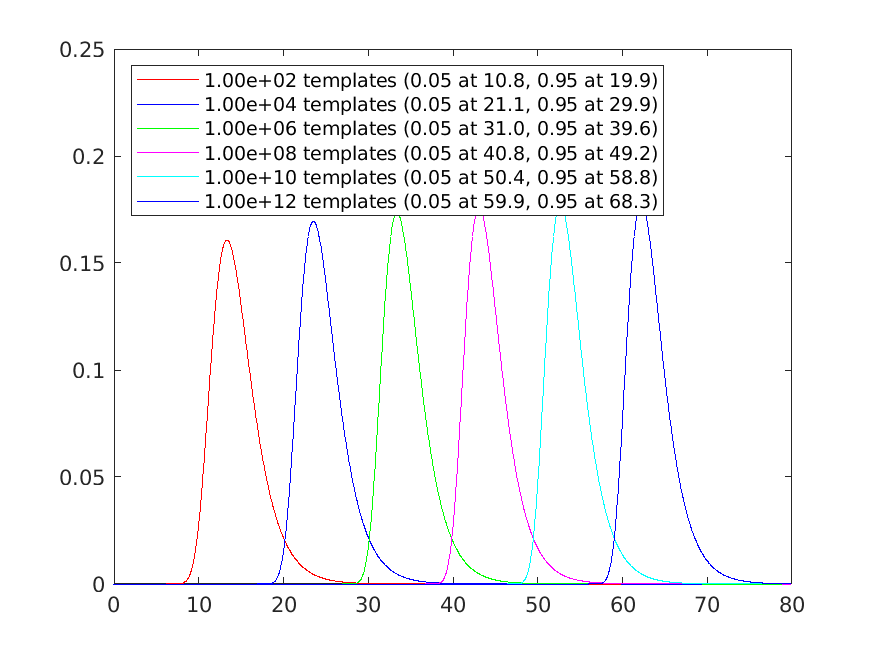
\includegraphics[width=\textwidth]{figure/2F_max.png}                  
        \caption{Image: Santiago Caride. Probability as a function of
                 $2\mathcal{F}$. The
                 plot shows clearly the $2\mathcal{F}$ value is a function of number of  templates.}                             
        \label{fig:2F_max}                                                  
\end{figure} 
The  $2\mathcal{F}$ at which the probability is highest are the most likely
values to be the loudest $2\mathcal{F}$. The plot ~\ref{fig:2F_max} shows the
$2\mathcal{F}$ values for which the probability is equal to $0.05$ and $0.95$.
Any $2\mathcal{F}$ below the $0.05$ mark has only a $5\%$ chance of being the
loudest; same for any $2\mathcal{F}$ above the $0.95$ mark.

These two values then give you a confidence interval we can say that, $95\%$ of
the time, the loudest  $2\mathcal{F}$ will lie between these two values. If the
loudest  $2\mathcal{F}$ from your search is not inside this interval, then it is
very unlikely to be Gaussian noise. That could mean that we found a signal, or
that we found a source of non-Gaussian noise, like an instrumental line or a
detector artifact. We would then have to do more detailed follow up on our
individual outliers to figure out which of those is the case.

\section{Veto process}
The interferometer data are contaminated from different noise sources. Some of
the noise sources are the instrument of interferometer(power supply, mirror
suspension, blinking LEDs, fans..) itself. These noises occurs in a specific
frequencies and might act as a signal for a continuous gravitational waves or
they can even mask the signals.  These noises known as instrumental lines need
to be properly identified and removed from the data searches. We will use a
Fscan veto to remove the frequency bands with instrumental lines. A Fscan is a
normalized spectogram form from the SFTs and normalize the SFTs by scaling the
power to the running median over 50 frequency bins~\cite{Aasi_2015}. If the
noise is stationary and Gaussian then the power is drawn from a $\chi^2$
distribution. If the fscan power deviates from the $\chi^2$ distribution, then
it is a non stationary Gaussian noise, spectral lines or both~\cite{Aasi_2015}.
It also gives a line width to a frequency of spectral lines depending on the
power of the lines. It looks for the frequency bins on either side that has
power less than half of the power of lines, the line width is subtracting the
below and above frequency vin of central frequency~\cite{Coughlin_2010}.

The other veto process is the interferometer veto. If the $2\mathcal{F}$ value
of any one of the detector is greater than the joint $2\mathcal{F}$ value of all
the detector, then such a $2\mathcal{F}$ will be discarded. 

\section{Upper limit}
If we didn't detect any signal($2\mathcal{F}<2\mathcal{F}^*$) then we set up an
upper limit on the intrinsic strain($h_0$) of the signal that we are trying to
detect~\cite{Romano_2017}. To calculate the upper limit, we need the
$2\mathcal{F}$ value and confidence level of our search on specific templates. 
So, for a confidence level of $95\%$, we would have detected a signal of
$2\mathcal{F}<2\mathcal{F}^*$ at least $95\%$ of the time~\cite{Romano_2017}. In
our pipeline, we calculate the value of $h_0$ such that the false dismissal rate
is 0.05 as shown in table ~\ref{table:UL}.
\begin{table*}                                                                  
\begin{center}                                                                  
\begin{tabular}{|c|c|}                                                           
\hline
\textrm{Intrinsic strain($h_0$)} & \textrm{$FDR$} \\                         
\hline
$3.84636\times10^{-25}$ & 0\\
$9.615891\times10^{-26}$ & 0.21 \\
$1.14081\times10^{-25}$ & 0.0772\\
$1.1911\times10^{-25}$ & 0.0528\\
$1.9795\times10^{-25}$ & 0.0501\\
$1.19809\times10^{-25}$ & 0.0501\\
\hline
\end{tabular}                                                                   
\end{center}                                                                    
\caption{Calculation of 95\% confidence level upper limits on the intrinsic strain ($h_o$)}                                                  
\label{table:UL}                                                        
\end{table*}                   
The upper limit on $r$-mode gravitational wave search of Crab pulsar will be
discussed later in Chapter .
%%%%%%%%%%%%%%%%%%%%%%%%%%%%%%%%%%%%%%%%%%%%%%%%%%%%%%%%%%%%%%%%%%%%%%%%%%%%%%%%%%%%%%%%%
%%%%%%%%%%%%%%%%%%%%%%%%%%%%%%%%%%%%%%%%%%%%%%%%%%%%%%%%%%%%%%%%%%%%%%%%%%%%%%%%%%%%%%%%%
%%% 							END OF FIFTH CHAPTER									  %%%
%%%%%%%%%%%%%%%%%%%%%%%%%%%%%%%%%%%%%%%%%%%%%%%%%%%%%%%%%%%%%%%%%%%%%%%%%%%%%%%%%%%%%%%%%
%%%%%%%%%%%%%%%%%%%%%%%%%%%%%%%%%%%%%%%%%%%%%%%%%%%%%%%%%%%%%%%%%%%%%%%%%%%%%%%%%%%%%%%%%

\chapter{\textbf{First searches for gravitational waves from $r$-modes of the
Crab pulsar}}

\section{Introduction}

Rapidly rotating neutron stars might be detectable emitters of long lived
quasi-monochromatic radiation known as continuous
\acp{GW}~\cite{Glampedakis2018}. The emission mechanism for continuous waves
could be a nonaxisymmetric mass quadrupole or a current-quadrupolar $r$-mode.
Hence the detection of continuous \acp{GW} might help reveal the underlying
properties of neutron star interiors. The \ac{GW} frequencies of many pulsars
lie in the most sensitive band of the \ac{LIGO}, so these rapidly rotating
neutron stars are attractive targets for continuous \ac{GW} searches.

The $r$-modes, whose frequencies are mainly determined by the Coriolis force,
are unstable to \ac{GW} emission~\cite{Andersson_1998,Friedman_1998} even
allowing for various damping mechanisms. Hence they might amplify and sustain
themselves, and might be the most interesting possibility for continuous
\acp{GW}. $R$-modes might play an important role in the spin-downs of the
fastest young neutron stars~\cite{Owen_1998} and in the regulation of spin
periods of some older accreting neutron stars. Comparison of the \ac{GW}
frequency to the spin frequency determined from timing radio or x-ray pulses
could measure the compactness of a pulsar.

Some \ac{GW} searches, starting with Ref.~\cite{Abadie_2010}, have set upper
limits on $r$-mode \ac{GW} emission.
However most of these have been broad band searches for neutron stars not
previously known as pulsars.
The searches themselves did not take any extra steps to account for $r$-mode
rather than mass-quadrupole emission; rather the results could be interpreted in
terms of $r$-modes~\cite{Owen_2010}.

Caride \textit{et al.}~\cite{Caride2019} showed that dedicated searches for
$r$-modes from known pulsars are feasible.
The key is to search the right range of frequencies and frequency derivatives,
which are significantly different from the more often considered case of
mass-quadrupole emission.
Not surprisingly, as with other \ac{GW} searches for pulsars, the Crab is the
first prospect to beat the spin-down limit using \ac{LIGO} data. The spin-down
limit assumes that all the rotational energy is
lost in the form of \acp{GW}, and represents a milestone a search must beat to
have a chance of detection.
Recently Fesik and Papa~\cite{Fesik2020} first published an $r$-mode pulsar
search similar to that proposed by Caride \textit{et al.}~\cite{Caride2019}, for another pulsar which is interesting for different reasons; but they
did not beat its spin-down limit.
The Crab is a relatively nearby pulsar with one of
the fastest known spin-down rates, and thus it has one of the highest spin-down
limits. Its rotational frequency changes at the rate
$-3.69\times10^{-10}$\,Hz/s~\cite{JodrellBankObservatory}. The Crab's pulse timing is constantly
measured by \ac{EM} observations, so the spin frequency evolution of the Crab is well known
during the LIGO \ac{O1} and \ac{O2}.

For various reasons we know that the Crab is not emitting \ac{GW} at or near the
spin-down limit.
Observations of the nebula indicate that most of the rotational energy is lost
powering the nebula via synchrotron and inverse Compton radiation from the
pulsar wind, and a few percent is lost in the narrow light
beam~\cite{B_hler_2014}. Recent \ac{GW} searches~\cite{Abbott_2019, O3}
have concluded that less than 0.01\% of the Crab's rotational energy loss is
through mass-quadrupole gravitational radiation.
The braking index $n$ of the Crab (the logarithmic derivative of its spin-down
with respect to frequency) is 2.519.
This is closer to the $n=3$ expected for magnetic dipole
radiation~\cite{Lyne_2014} than to the $n=7$ expected for
$r$-mode emission~\cite{Owen_1998}.
Such a low braking index is another indicator that \ac{GW} emission is a small
fraction of the spin-down limit.
How small has not been quantified in a model-independent way or for $r$-modes.
But Palomba~\cite{Palomba2000} found that, for a class of reasonable
mass-quadrupole models, the measured braking index of the Crab means it is
emitting \ac{GW} at least a factor of a few below the spin-down limit.
We take this to suggest that any $r$-mode \ac{GW} signal from the Crab must be
at least a factor of a few (in strain) below the spin-down limit.

Nevertheless, Caride \textit{et al.}~\cite{Caride2019} showed that a search of
the Crab with interesting sensitivity is feasible, and we confirm this.
We performed searches for the Crab in  \ac{O1} and \ac{O2} data (the publicly
available LIGO data sets) using the matched filtering-based technique known as
the F-statistic.
While we did not find any evidence of a \ac{GW} signal, we were able to set
upper limits beating the spin-down limit by a significant amount over a wide
parameter space.

\section{R-modes search method} 

Our search consists of a matched filtering technique to extract a signal from a
detector noise known as $\mathcal{F}$-statistic. The $\mathcal{F}$-statistic
developed by ~\citet{Jaranowski_1998} for single interferometer and by
~\citet{PhysRevD.72.063006} for multi interferometer is a statistical procedure
for the detection of the continuous gravitational waves. The
$\mathcal{F}$-statistic accounts for the Doppler and amplitude modulation due
to the daily rotation and orbital motion of Earth in a computationally efficient
manner. In the presence of signal,
the $2\mathcal{F}$ is a non-central chi squared distribution with four degrees
of freedom and the non-central parameter is proportional to the signal. The
$\mathcal{F}$-statistic is the log of the maximum likelihood function over the
unknown parameter: amplitude strain, phase constant, inclination angle and
polarization angle. 
The main issue, as described by Caride \textit{et al.}~\cite{Caride2019}, is to
find the ranges of frequencies and frequency derivatives to search.

Pulsars are slowly spinning down due to \ac{GW} and other losses of rotational
energy. The \ac{GW} frequency evolution of a spinning down neutron star in the
frame of the solar system barycenter is approximated by: 
\begin{equation}
 \nu(t) = \nu\left( t_0 \right) + \dot{\nu}\left( t_0 \right) \left( t-t_0
\right) + \frac{1}{2} \ddot{\nu}\left( t_0 \right) \left( t-t_0 \right)^2,
\end{equation} 
where $t_0$ is a reference time, often the start time of the observation.
Generally $\dddot{\nu}$ is not needed for a less than a year of integration
time~\cite{Caride2019}. The frequency evolution is precisely known from
electromagnetic observations. It might depart from the above evolution due to
timing noises or glitches. Glitches are sudden increases in spin frequency
followed by exponential recovery to the pre-glitch
frequency~\cite{Espinoza_2011}. Timing noise is residual phase wandering of
pulses
relative to the normal spin down model.
Since the Crab glitched during O2, we divided the search into two roughly equal
stretches. More on the Crab pulsar timing for our search will be discussed in
section~\ref{timing}.

For long duration searches the signals can be affected by timing noise. Timing
noise will deviate \ac{GW} phases from Taylor series for time scales of 1 year
and longer~\cite{Jones_2004}. Assuming, the \ac{GW} timing noise is similar to
the one observed in EM pulses, the mismatch of the Crab ephemeris during LIGO S5
run from the model with no timing noise is less than
$1\%$~\cite{PhysRevD.91.062009}.  So, for all our searches (four months of
data), timing noises should not significantly mismatch the templates from
signal.

For a Newtonian star with spin frequency $\nu$, the $r$-mode \ac{GW} frequency is approximately $f=\frac{4}{3}\nu$. The frequency ratio
deviates from $4/3$ when corrections due to general relativity, rapid rotation,
magnetic fields and core-crust coupling are considered~\cite{Idrisy:2014qca}.
For fast rotating neutron stars, the elastic restoring force on the crust
couples with the Coriolis restoring $r$-modes resulting in avoided
crossings~\cite{Levin_2001}. These are small frequency bands where the simple
relation between f and $\nu$ is drastically altered as modes change identities.
Away from avoided crossings, the $r$-mode frequency as a function of spin
frequency is approximately
\begin{equation}
f=A\nu-B\left(\frac{\nu}{\nu_K}\right)^2, 
\end{equation} 
where $\nu_K$ is the Kepler frequency. Here we neglect other effects so that A
and B are the general relativistic and slow rotation corrections.  
As the modes are retrograde in rotating frame but prograde in inertial frame,
the General relativity correction decreases the mode frequency in a co-rotating
frame but increases in an inertial frame.  Since,the modes restoring force is
Coriolis force which is given by the fluid angular velocity relative to the
local inertial frame $(\tilde\omega=\Omega - \omega)$, the modes oscillates less
rapidly when frame dragging effect is
significant~\cite{Lockitch:2000aa,1968ApJ...153..807H}. The effect of rapid
rotation is to decrease the mode frequency in an inertial frame.  The
gravitational redshift decreases the mode frequency as clock will be ticking
slower in relativistic case as seen by the distant observer. 

The range of A and B is chosen as follows: We consider a range of compactness of
neutron stars ($0.11\leq M/R\leq 0.31$)~\cite{Idrisy:2014qca} which comes from
the uncertainty in the equation of state. The range on compactness gives a range
$1.39\leq A \leq 1.57$. The range on B are derived from the relation of $f/\nu$
to the ratio of the rotational energy (T) to the gravitational potential energy
(W)~\cite{Yoshida:2004gk}. For different polytropic index and the compactness,
the range is 1.23-1.95 times the rotational parameter(T/W). \citet{Caride2019}
converted T/W into a $(\nu/\nu_k)^2$ using a $M/R=0.1$ that gives a maximum
value of B = 0.195. The minimum value of B is not well known so written as 0. 
The range on A and B is
\begin{equation}
 A=(1.39-1.57) \quad \& \quad B=(0-0.195), 
\end{equation}

Our search consists of parameter $f$, $\dot{f}$, $\ddot{f}$ that makes a
template of \ac{GW}. The distance between two templates is given by minimal
match ($\mu$) which is the loss in signal to noise ratio when signal falls
exactly between two theoretical waveforms~\cite{Owen:1995tm}.  
The parameter space for our search is given by \citet{Caride2019}:
\begin{eqnarray}
\nu \left[ A_{\min} - B_{\max} \left( \nu/\nu_K \right)^2 \right] & \le & f
\le \nu\, A_{\max},
\\
\dot\nu \left[ f/\nu - 2B_{\max} \left( \nu/\nu_K \right)^2 \right] & \le &
\dot f \le \dot\nu f/\nu,
\\
0 & \le & \ddot f \le \ddot\nu f/\nu,
\end{eqnarray}
where, $f$ is spin frequency, $\dot{f}$ and $\ddot{f}$ is the first and second
spin derivative.

We use the parameter space metric $g_{ij}$ to control the computational
cost of our search. 
The parameter space metric is given by~\cite{Wette:2008hg,Owen:1995tm}:
\begin{equation}
g_{ij}=\frac{4\pi^2T^{i+j+2}(i+1)(j+1)}{(i+2)!(j+2)!(i+j+3)}
\end{equation}\\
where i, j stands for parameters $(f,\dot{f},\ddot{f})=(0,1,2)$ and T is the time spanned by the observation. 
The template number is given by dividing the proper volume of the parameter
space by the proper volume per template:~\cite{Caride2019}
\begin{equation}\label{templatescalc}
Templates = \frac{\sqrt{g} \nu \left| \dot\nu \right| \ddot\nu B_{\max} \left(
\nu/\nu_K
\right)^2 \left[ A_{\max}^2 - A_{\min}^2 \right]}{\left( 2 \sqrt{\mu/3}
\right)^3}
\end{equation}

We look at the search jobs with the highest value of $\mathcal{F}$-statistic
($2\mathcal{F}^*$) that survived the automated vetoes. The probability that the
given value of $2\mathcal{F}^*$ will be observed when no signal are present is
given by~\cite{Abadie_2010}: 
\begin{equation} 
p(N;2\mathcal{F}^*)= Np(\chi^2_4;2\mathcal{F}^*)[cdf(\chi^2_4;2\mathcal{F}^*)]^{N-1} 
\end{equation} 
where N is the number of templates and $p(\chi^2_4;2\mathcal{F}^*)$ is the
central $\chi^2$ distribution with four degrees of freedom.  A high
$2\mathcal{F}$ is not enough to claim the detection, as instrumental lines might
act as a periodic signal. A search is followed by the F-scan veto and
interferometer consistency veto that remove narrow band instrumental
lines~\cite{Lindblom_2020}. F-scan looks for lines by normalizing the
\acp{SFT}  using a running median of 51 frequency bins.  Then the interferometer
veto is applied which discards the templates when the joined $2\mathcal{F}$
value from the two interferometer is less than any of the single interferometer.

%where i,j are the indices for frequency and its derivatives
%labeled as
%$(f,\dot{f},\ddot{f})=(0,1,2)$.~\cite{PhysRevD.100.064013}\cite{Wette:2008hg}
%For the pulsars and integration time of interests, both $f$ and $\dot{f}$
%parameters are 
%necessary to build  the \ac{GW} template.  The requirement of $\ddot{f}$ depends
%on the mismatch between the signals and waveform when the $\ddot{f}$ is ignored.
%For the continuous \ac{GW} search the maximum mismatch between template and
%signal is 0.2, i.e. we won't lose more than $20\%$ of signal to noise ratio
%$\ddot{f}$ is necessary. If the mismatch  $g_{22}\ddot{f}^2 >0$ $\ddot{f}$ is
%necessary. Using the maximum $\ddot{f}$ observed during our search,and with $T=
%10^7s(O1)$ $g_{22}\ddot{f}$ = $5.5$, so $\ddot{f}$ is a requirement. 
	

\section{The Crab pulsar} \label{timing}
The Crab pulsar is the remnant of a supernova explosion seen by
Chinese astronomers in the year 1054 AD. This is our first target due to its
high spin down limit which is  well above the LIGO \ac{O1} noise
curve~\cite{Caride2019}. The rotational energy loss of the
pulsar is given by $\dot{E}=4\pi^2I_{zz}\nu\dot{\nu}\approx 4.33\times10^{31}W$
,where $(I_{zz}=10^{38}kg m^2)$ is the principal moment of inertia ~\cite{Abbott_2008}. The spin-down power of the Crab is high enough that, even if
$r$-mode gravitational wave emission is only responsible for a small fraction of
it, the \acp{GW} could be detectable.
 
The sky location of Crab pulsar in J2000 coordinates is~\cite{1993MNRAS.265.1003L} 
\begin{equation}
\begin{aligned} 
\alpha =05^h34^m31.94^s\\ 
\delta=
+22^\circ00^\prime52.1^{\prime\prime} 
\end{aligned} 
\end{equation}
 
The spin frequency and its derivative~\cite{1993MNRAS.265.1003L} were obtained
from the Jodrell Bank observatory monthly ephemeris and interpolated to the
start dates of the LIGO run from the nearest dates of 09/16/2015 (\ac{O1}),
11/23/2016 (early O2) and 04/16/2017 (late O2). There were no glitches of the
Crab during \ac{O1}, so the whole run can be coherently integrated. The Crab
glitched at 2017-03-27 22:04:48.000 UTC~\cite{Espinoza_2011} during the \ac{O2}
run, approximately halfway through. So we divided the \ac{O2} run into two
roughly equal stretches.  The glitch was comparatively small
($\frac{\Delta\nu}{\nu}= 2.14\times 10^{-9}$)~\cite{Espinoza_2011} and the
relaxation time period for the glitches are not well known, so we started the
search of late \ac{O2} a few hours afterwards.

Fast spinning down pulsars are contaminated by timing
noise~\cite{Lyne1992GlitchesAP} specially when $\ddot{\nu}$ is negative. During
our observational time, the monthly $\ddot{\nu}$ measurement was fluctuating.
This might be due to external torque from magnetosphere. So, we chose the
maximum $\ddot{\nu}$ as maximum value observed during the observational time and
minimum $\ddot{\nu}$ as zero. The extra number of templates required by
including $\ddot{\nu}$ is factor of a few, so the searches will not be too
expensive if we made $\ddot{\nu}$ from $0$ to a maximum seen value of
$\ddot{\nu}$. 
\begin{table*} 
%\begin{ruledtabular}
\begin{tabular}{ cccccc} 
\textrm{Search} & \textrm{Start time(UTC)} & \textrm{End time(UTC)} &
\textrm{Time span(days)} &  \textrm{Obs.Time(days)} & \textrm{SFTs}\\ 
%\colrule
\textrm{\ac{O1}} & 09/12/15(06:03:57) & 01/19/16(15:34:47) & 129.36 & 66.55 &6389\\ 
\textrm{\ac{O2}(early)} & 11/30/16(18:01:57) & 03/27/17(16:28:25) &  116.93 &
56.167 & 6186\\ 
\textrm{\ac{O2}(late)} & 03/28/17(23:47:38) & 08/25/17(21:59:34) & 149.92 & 74.9 &
8035 \\ 
\end{tabular} 
%\end{ruledtabular}
\caption{The start and end times of the three searches.  The observational time
is the total duration of \acp{SFT}(1800s each) divided by the number of
interferometers (H1 \& L1).}
\label{table:Time} 
\end{table*} \\

\begin{table} 
%\begin{ruledtabular}
\begin{tabular}{cccc } 
\textrm{Search} & \textrm{$\nu$} &\textrm{$\dot{\nu}$} & \textrm{$\ddot{\nu}$}\\ 
%\colrule
\ac{O1} & $29.66181$ & $-3.69383\times10^{-10}$ &  $2.41\times10^{-20}$\\ 
\ac{O2}(pre-glitch) & $29.64761$ & $-3.689673\times10^{-10}$ & $1.92\times10^{-20}$\\ 
\ac{O2}(post-glitch) & $29.6438$ & $-3.688438\times10^{-10}$ &  $2.5\times10^{-20}$\\ 
\end{tabular} 
%\end{ruledtabular}
\caption{Timing of Crab pulsar at the beginning of our three different searches.
The timing is measured by Jodrell Bank Observatory~\cite{1993MNRAS.265.1003L}
and interpolated to the start time of LIGO run. The recorded $\ddot{\nu}$ is the
maximum value observed for the period of three different run.}
\label{table:timing} 
\end{table} 

\section{Implementation} 
We used data from the \ac{GWOSC}, starting with time-domain strain data sampled
at 4\,kHz.  We downloaded all such \ac{O1} data for the official duration of the
run (from GPS times 1126051217 to 1137254417) from both interferometers (H1 and
L1), gating on only ``CBC CAT1'' vetoes.  These indicate disastrous conditions
for the instruments, such as loss of laser power.  We ignored the other vetoes
used in searches for binary black holes and neutron stars because they are aimed
at short-duration disturbances which are not an issue for continuous wave
searches.  We then used the code \texttt{lalapps\_MakeSFTDAG} from LALSuite to
generate 1800\,s long \acp{SFT}, version\,2, high pass filtered with a knee
frequency of 7\,Hz and windowed with the default Tukey window.  This produced
6,389 \acp{SFT} for \ac{O1} (3,474 from H1 and 2,915 from L1).  A similar
procedure for \ac{O2} produced 14,231 \acp{SFT} (7,242 from H1 and 6,989 from
L1).  Our $r$-mode search used a modified version of Supernova remnant
pipeline\cite{Aasi_2015} and ``Texas Tech University High Performance Computing
Center'' for computational power.

The frequency band of the search are 41.2 - 46.6 Hz (O1) and 41.1 -46.6 Hz (O2).
The minimum and maximum frequencies are rounded down and up to the one decimal
of place. This is because the frequency band needs to be a frequency resolution
of 0.1 Hz. We use a bank of template with minimal match is 0.2. The ideal
template number for Crab O1, early O2 and late O2 are $2.27\times 10^9$,
$9.71\times 10^8$ and $4.02\times 10^9$ respectively. The actual search produced
$1.72\times 10^{10}$, $1.17\times 10^{10}$ and $3.62 \times 10^{10}$ templates.
The number of templates of search is around an order of magnitude greater than
the ideal templates calculated. This is because the search uses extra templates
to cover the boundaries outside the parameter space~\cite{Abadie_2010}. The
O1, early O2 and late O2 used computational time of 1584, 944 and 3892 core
hours. 

%\begin{table}
%\begin{ruledtabular}
%\begin{tabular}{ccc} 
% \textrm{Search} & \textrm{Template Density} & \textrm{Search Jobs (core hrs)} \\ 
%\colrule
%\ac{O1} & 3202057000 & 1584\\
%\ac{O2}(pre-glitch)  & 2129421000 & 944\\ 
%\ac{O2}(post-glitch) & 6587981400 & 3892 \\
%\end{tabular} 
%\end{ruledtabular}
%\caption{Computational cost}\label{cost} 
%\end{table} 


\begin{table*} 
%\begin{ruledtabular}
\begin{tabular}{cccc} 
  \textrm{Search} & \textrm{Search bands} & \textrm{Vetoed bands} & \textrm{Fraction of band searched}\\   
%\colrule  
\ac{O1} & 5.4 Hz & 1.286 Hz & 0.76\\ 
\ac{O2}(pre-glitch)& 5.5 Hz  & 0.79 Hz & 0.85\\ 
\ac{O2}(post-glitch) & 5.5 Hz & 1.33 Hz & 0.758\\  
\end{tabular} 
%\end{ruledtabular}
\caption{Total vetoed frequency band of the search due to instrumental
lines}\label{table:veto} 
\end{table*} 
 
The F-scan veto threshold was fixed to twenty standard
deviations.  We set threshold of 33 for $2\mathcal{F}$, any $2\mathcal{F}$ below
it will be discarded.  The total frequency band vetoed are 1.29 Hz (O1), 0.79 Hz
(early O2) and 1.33 Hz (late O2). This is about $75\%$ (O1), $85\%$ (early O2)
and $76\%$ (late O2) of the total frequency band searched. We set the false
alarm probability as $5\%$. If the $2\mathcal{F}$
value from the search has less than 5\% chance of being drawn from
$p(2\mathcal{F}^*)$ then it is the first step to claim the \ac{GW} signal. None
of the non-vetoed templates had a $2\mathcal{F}$ value that beat the 95\%
significance level so no detection was made in all our search.

\section{Upper limit}
In the absence of a detection, we set an upper limit gravitational wave
emission. The method is similar to ~\citet{Lindblom_2020}. Upper limit are the
weakest signal that can be detected from our search with certain probability.
The frequentist upper limit depends on the observed $2\mathcal{F}$ value and the
choice of confidence level. For our case, the upper limit is $95\%$ confidence
level, i.e. for a minimum $h_o$, $2\mathcal{F} > 2\mathcal{F}^*$ $95\%$ of the
time~\cite{Romano_2017}. This means we set the false dismissal rate to $5\%$,
and the loudest $2\mathcal{F}$ observed will set the false alrm
rate~\cite{Aasi_2015}. The upper limit bands are chosen to be small enough for
the interferometer noise to stay constant. The upper limit band for all the
searches is 0.1 Hz. 

First, we use a computationally inexpensive Monte Carlo to determine the loudest
non-vetoed $2\mathcal{F}$ and find a $95\%$ confidence level intrinsic strain
($h_o$) that gives such a $2\mathcal{F}$. Then we use computationally expensive
($20- 30\%$ of the cost of search)~\cite{Aasi_2015} software injection searches
to make the validation of the upper limit. 1000 fake signals with fixed $h_o$
(that was determined in previous step) and variable $f,\dot{f},\ddot{f}$ and
other unknown parameters are injected in each upper limit band to check the
validity of $h_o$. The maximum value of $2\mathcal{F}$ obtained from the
injection is compared to the $2\mathcal{F}^*$ from the search results. If
$2\mathcal{F}> 2\mathcal{F}^*$ then this $h_o$ will be our upper limit.  The
upper limit of intrinsic strain and $r$-mode amplitude for our three searches is
shown in figure ~\ref{fig:UL}.  The best $95\%$ confidence level upper limits on
intrinsic amplitude strain of our search are $1.61\times 10^{-25}$ (O1),
$1.45\times 10^{-25}$ (early O2) and $1.20\times 10^{-25}$ (late O2). The upper
limit for the searches beats the spin down limit by order of magnitude in
amplitude strain and two orders of magnitude in luminosity. 

We can also set upper limits on $r$-mode amplitude.  
The derivation of $r$-mode amplitude ($\alpha$) is shown by \citet{Owen_2010},
who took the fiducial value of moment of inertia $(I_{zz})=10^{38}kgm^2$
and typical $M=1.4M_\odot$. We convert the upper limit on
intrinsic strain ($h_o$) to a r-mode amplitude ($\alpha$).   
\begin{equation} 
\alpha
=0.028\left(\frac{h_o}{10^{-24}}\right)\left(\frac{r}{1kpc}\right)\left(\frac{100Hz}{f}\right)^3
\end{equation} 

The best $r$-mode amplitude upper limits for our different searches are $0.0898$
(O1), $0.082$ (early O2) and $0.067$ (late O2). 
%The millisecond pulsar will have $\alpha$ from $10^{-6}$
%- $10^{-4}$, some might have as high as 0.01~\cite{Owen_2010}. The saturation
%  amplitude of unity spins down the pulsar to a one-tenth of its rotational
%velocity in a year~\cite{Lindblom_2001}. And neutron star with low saturation
%amplitude might not be spinning down due to $r$-modes.


\begin{figure}[h!] 
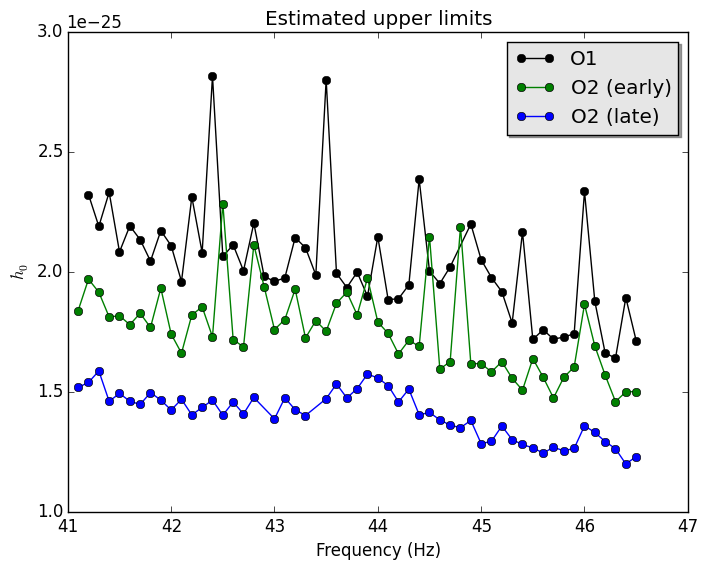
\includegraphics[width=3in]{Crabupper.png}
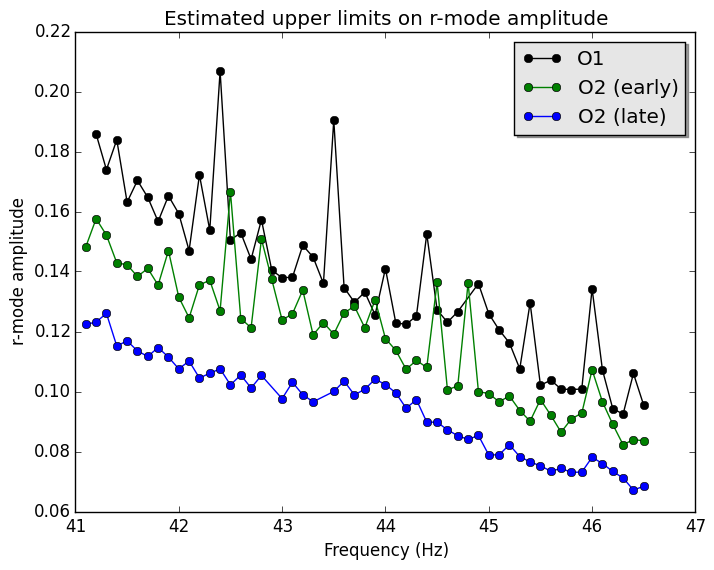
\includegraphics[width=3in]{modeamplitude.png}

\caption{Comparison of upper limits on intrinsic strain (left) and $r$-mode
amplitude (right) for our three searches. The late search is the most sensitive one as it has the more observational
time and detectors were more sensitive later.} 
\label{fig:UL}
\end{figure}

%\begin{table*} 
%\begin{center} 
%\begin{ruledtabular}
%\begin{tabular}{ ccc} 
% \textrm{Search} & \textrm{$h_o$} & \textrm{$\alpha$}\\  
%\colrule 
%\ac{O1} & $1.61\times 10^{-25}$ & 0.0898\\ 
%\ac{O2}(pre-glitch) & $1.45\times 10^{-25}$ & 0.082\\ 
%\ac{O2}(post-glitch) & $1.20 \times 10^{-25}$ & 0.067\\  
%\end{tabular} 
%\end{ruledtabular}
%\end{center} 
%\caption{95\% confidence level upper limits on the intrinsic strain ($h_o$) and
%$r$-mode amplitude ($\alpha$)}
%\label{table:upperlimit} 
%\end{table*}

\section{Conclusion} 

Our search for Crab pulsar didn't detect $r$-mode \acp{GW} from \ac{LIGO}
\ac{O1} and \ac{O2} run. The second run of \ac{O2} has the better sensitivity
mostly due to the longer observational time and both interferometer were taking
data simultaneously. Although, the spin down limit of Crab is higher, the \ac{GW}
amplitudes might not be high enough to beat the LIGO sensitivity. The longer
observational time and better sensitivity might be able to detect continuous
\ac{GW} in future LIGO run.  We will extend our search of Vela pulsar which
beats the spin down limit for the LIGO \ac{O2} run.  

J0537-6910 might be another interesting pulsar as the average inter-glitch
braking index is closer to 7 when subtracting the exponential decay component of
$\dot{nu}$ during the glitch recoveries~\cite{Andersson_2018,Ferdman_2018}, this
means  it might be spinning down due to $r$-mode \ac{GW} emission. We do not
have a timing of this pulsar during the \ac{O1} and \ac{O2} run and it glitches
almost every 100 days, so longer observational time will mismatch the signal
with the theoretical templates. The $r$-mode \ac{GW} from J0537-6910 pulsar has
recently been searched by ~\citet{Fesik2020}, using the timing from Rossi
X-ray Timing Explorer from Nov 2011 and interpolating to the LIGO \ac{O1} and
\ac{O2} run. They have considered two scenarios where $r$-modes is active or
shuts off just on the beginning of observation. The search didn't find any
evidence of $r$-modes.  

Some nearby pulsar J0437-4715 and J0711-6830 are important due to its proximity
and its frequency lies where \ac{LIGO} is more sensitive. But its spin down
frequency are very low $(10^{-15})$, so its spin down limit only beats LIGO A+
noise curve. J0437-4715 is a billion years old pulsar but its temperature is
more than expected for a old pulsar, so some astronomers thinks there might be
some internal heating mechanism~\cite{Durant_2012} increasing the temperature of
neutron star and $r$-modes heating might be one of the factor. Both J0437-4715
and J0711-6830 spin down limits are well below the LIGO \ac{O1} and \ac{O2}
noise curve so the search might only be important for the future LIGO run.  



%%%%%%%%%%%%%%%%%%%%%%%%%%%%%%%%%%%%%%%%%%%%%%%%%%%%%%%%%%%%%%%%%%%%%%%%%%%%%%%%%%%%%%%%%
%%%%%%%%%%%%%%%%%%%%%%%%%%%%%%%%%%%%%%%%%%%%%%%%%%%%%%%%%%%%%%%%%%%%%%%%%%%%%%%%%%%%%%%%%
%%%                                                     END OF SIXTH CHAPTER
%%%%
%%%%%%%%%%%%%%%%%%%%%%%%%%%%%%%%%%%%%%%%%%%%%%%%%%%%%%%%%%%%%%%%%%%%%%%%%%%%%%%%%%%%%%%%%
%%%%%%%%%%%%%%%%%%%%%%%%%%%%%%%%%%%%%%%%%%%%%%%%%%%%%%%%%%%%%%%%%%%%%%%%%%%%%%%%%%%%%%%%%


\chapter{\textbf{Conclusion}}
This thesis presents the work on $r$-mode \ac{GW} searches from a Crab pulsar
for the \ac{LIGO} \ac{O1}and \ac{O2} run. We also showed the right frequency
parameter and estimated computational cost for the $r$-mode search. In chapter 1
we started discussing about some of the historic discovery of \acp{GW} by
\ac{LIGO} and Virgo interferometer. Then in chapter 2 we derived the Einstein
field equation and showed the perturbation in flat space-time travels at speed
of light known as gravitational waves. Then, we described the polarization of
\acp{GW} and energy radiated from \ac{GW} emission.  The principal of \acp{GW}
detector is based on the Michelson interferometer. The interferometer are
affected by various noise sources, we mentioned some origin of the noises and
the steps to extract signals that are buried in noise. We gave a details on
neutron star structure and emission of \ac{GW} radiation due to mountains on
neutron stars.

In chapter 3 we talked about the $r$-mode emission from a rotating neutron star.
R-modes are damped by the viscous mechanism but are unstable to \ac{GW}
radiation. We discussed the dependence of $r$-mode
instability window to the temperature and spin frequency of neutron star. We
later explained the $r$-mode frequency deviate from Newtonian case due to the
correction from general relativity and rapid rotation. 

Chapter 4 shows the correct frequency band and frequency derivatives to search
for $r$-modes. The right parameter is derived using the first and second order
correction in $r$-modes frequencies. The correction includes but not limited to
unknown compactness of neutron star and rapid rotation correction.  The chapter
also includes the spin down limit of selected pulsar that beats the LIGO noise
curve. Crab has the best spin down limit in terms of intrinsic strain and it can
be the first pulsar to search for $r$-mode \acp{GW}. 

In chapter 5 we discussed the method of extracting continuous wave signals from
the \ac{LIGO} noisy data. We started by the interferometer response to the
\ac{GW} signal and how the continuous wave signal are the functions of Doppler
and Amplitudes parameter. Then we gave a brief introduction of maximum
likelihood functions and how the signals are maximized to the unknown amplitude
parameters. We gave details of construction of \ac{SFT} and waveforms
from the interferometer data for the continuous waves. To claim the signal
detection, the signal should be above a certain confidence level. If there is a
signal in the data, the expected $\mathcal{F}-statistic$ value will be the non
central chi squared deviation, where the non central parameter will be
proportional to the signal. 

The next chapter is about the $r$-mode \ac{GW} search from the Crab pulsar. On
chapter 4 we gave a details why Crab is our first candidate. The Crab pulsar
timing has been constantly monitored by the Jodrell Bank Observatory. We
searched for a first two observing run of a Advanced \ac{LIGO}. Crab glitched in
the middle of the second run, so we divided the second \ac{LIGO} run into two
halves. We described the process of data analysis in our search that are
explained in detail in chapter 5. We did not find any evidence of \ac{GW} so, we
set up the upper limit for the three different searches.   

With the improvement of \ac{LIGO} sensitivity and computational power in few
years, the detection of continuous gravitational wave will be more probable. The
better understanding of $r$-mode instability and saturation amplitude will also
help to know the energy of the $r$-mode gravitational wave emission. Since, the
detection of continuous \ac{GW} will help us to understand the neutron star
structure, this will benefit not only the astronomer but nuclear and particle
physicist too.
%%%%%%%%%%%%%%%%%%%%%%%%%%%%%%%%%%%%%%%%%%%%%%%%%%%%%%%%%%%%%%%%%%%%%%%%%%%%%%%%%%%%%%%%%
%%%%%%%%%%%%%%%%%%%%%%%%%%%%%%%%%%%%%%%%%%%%%%%%%%%%%%%%%%%%%%%%%%%%%%%%%%%%%%%%%%%%%%%%%
%%% 						End of Fifth Chapter 											  %%%
%%%%%%%%%%%%%%%%%%%%%%%%%%%%%%%%%%%%%%%%%%%%%%%%%%%%%%%%%%%%%%%%%%%%%%%%%%%%%%%%%%%%%%%%%
%%%%%%%%%%%%%%%%%%%%%%%%%%%%%%%%%%%%%%%%%%%%%%%%%%%%%%%%%%%%%%%%%%%%%%%%%%%%%%%%%%%%%%%%%







%%%%%%%%%%%%%%%%%%%%%%%%%%%%%%%%%%%%%%%%%%%%%%
%Backmatter -- Bibliography, appendices, etc.%
%%%%%%%%%%%%%%%%%%%%%%%%%%%%%%%%%%%%%%%%%%%%%%
\backmatter


%%%%%%%%%%%%%%%%%%%%%%%%%%%%%%%%%%%%%%%%%%%%%%%%%%%%%%%%
%Bibliography:  Use BibTeX 							   %
%%%%%%%%%%%%%%%%%%%%%%%%%%%%%%%%%%%%%%%%%%%%%%%%%%%%%%%%
\bibliographystyle{plain}
\addcontentsline{toc}{chapter}{\textbf{References}}
\bibliography{thesis}


%%%%%%%%%%%%%%%%%%%%%%%%%%%%%%%%%%%%%%%%%%%%%
%        APPENDIX A                         %
%%%%%%%%%%%%%%%%%%%%%%%%%%%%%%%%%%%%%%%%%%%%%
%\appendix
%\label{swpn}
%\addtocontents{toc}{\noindent\hyperref[swpn]{\textbf{Appendices}}}
%\addcontentsline{toc}{chapter}{A. \textbf{Double T Signature}}
%\chapter*{ } 	%Define an empty chapter title placeholder
%\vspace*{\fill}
%\begin{center}\textbf{Appendix A}\end{center}
%\begin{center}\textbf{Double T Signature}\end{center} %make sure the appendix title matches the title in the \addcontentsline portion above!
%\vspace*{\fill}
%
%
%\renewcommand\thefigure{A.\arabic{figure}} %this is to label the figure number using the Appendix name "A" instead of Chapter 6
%
%\afterpage{
%\begin{figure}
%\centering
%\includegraphics[width=\textwidth]{TTU_DblTalt_c2C.pdf}
%\caption{Double T signature}
%\label{fig:doubleT_sig}
%\end{figure}
%\clearpage
%}
%
%%%%%%%%%%%%%%%%%%%%%%%%%%%%%%%%%%%%%%%%%%%%%%
%%        APPENDIX B                         %
%%%%%%%%%%%%%%%%%%%%%%%%%%%%%%%%%%%%%%%%%%%%%%
%\addcontentsline{toc}{chapter}{B. \textbf{Another Double T}}
%\chapter*{\textbf{ }}
%\vspace*{\fill}
%\begin{center}\textbf{Appendix B}\end{center}
%\begin{center}\textbf{Another Double T}\end{center} %make sure the appendix title matches the title in the \addcontentsline portion above!
%\vspace*{\fill}
%
%\renewcommand\thefigure{B.\arabic{figure}}
%\setcounter{figure}{0}
%\afterpage{
%\begin{figure}
%\centering
%
\includegraphics[width=\textwidth]{TTU_DblT_fl4Crvs.jpg}
%\caption{Another Double T}
%\label{fig:doubleT_sig2}
%\end{figure}
%\clearpage
%}
%


\end{document}




